% Options for packages loaded elsewhere
\PassOptionsToPackage{unicode}{hyperref}
\PassOptionsToPackage{hyphens}{url}
%
\documentclass[
]{article}
\usepackage{lmodern}
\usepackage{amssymb,amsmath}
\usepackage{ifxetex,ifluatex}
\ifnum 0\ifxetex 1\fi\ifluatex 1\fi=0 % if pdftex
  \usepackage[T1]{fontenc}
  \usepackage[utf8]{inputenc}
  \usepackage{textcomp} % provide euro and other symbols
\else % if luatex or xetex
  \usepackage{unicode-math}
  \defaultfontfeatures{Scale=MatchLowercase}
  \defaultfontfeatures[\rmfamily]{Ligatures=TeX,Scale=1}
\fi
% Use upquote if available, for straight quotes in verbatim environments
\IfFileExists{upquote.sty}{\usepackage{upquote}}{}
\IfFileExists{microtype.sty}{% use microtype if available
  \usepackage[]{microtype}
  \UseMicrotypeSet[protrusion]{basicmath} % disable protrusion for tt fonts
}{}
\makeatletter
\@ifundefined{KOMAClassName}{% if non-KOMA class
  \IfFileExists{parskip.sty}{%
    \usepackage{parskip}
  }{% else
    \setlength{\parindent}{0pt}
    \setlength{\parskip}{6pt plus 2pt minus 1pt}}
}{% if KOMA class
  \KOMAoptions{parskip=half}}
\makeatother
\usepackage{xcolor}
\IfFileExists{xurl.sty}{\usepackage{xurl}}{} % add URL line breaks if available
\IfFileExists{bookmark.sty}{\usepackage{bookmark}}{\usepackage{hyperref}}
\hypersetup{
  pdftitle={Supplementary Materials: Details on Data, Analyses, and Reproduction of Tables and Figures},
  pdfauthor={Justin M. Leach},
  hidelinks,
  pdfcreator={LaTeX via pandoc}}
\urlstyle{same} % disable monospaced font for URLs
\usepackage[margin=1in]{geometry}
\usepackage{color}
\usepackage{fancyvrb}
\newcommand{\VerbBar}{|}
\newcommand{\VERB}{\Verb[commandchars=\\\{\}]}
\DefineVerbatimEnvironment{Highlighting}{Verbatim}{commandchars=\\\{\}}
% Add ',fontsize=\small' for more characters per line
\usepackage{framed}
\definecolor{shadecolor}{RGB}{248,248,248}
\newenvironment{Shaded}{\begin{snugshade}}{\end{snugshade}}
\newcommand{\AlertTok}[1]{\textcolor[rgb]{0.94,0.16,0.16}{#1}}
\newcommand{\AnnotationTok}[1]{\textcolor[rgb]{0.56,0.35,0.01}{\textbf{\textit{#1}}}}
\newcommand{\AttributeTok}[1]{\textcolor[rgb]{0.77,0.63,0.00}{#1}}
\newcommand{\BaseNTok}[1]{\textcolor[rgb]{0.00,0.00,0.81}{#1}}
\newcommand{\BuiltInTok}[1]{#1}
\newcommand{\CharTok}[1]{\textcolor[rgb]{0.31,0.60,0.02}{#1}}
\newcommand{\CommentTok}[1]{\textcolor[rgb]{0.56,0.35,0.01}{\textit{#1}}}
\newcommand{\CommentVarTok}[1]{\textcolor[rgb]{0.56,0.35,0.01}{\textbf{\textit{#1}}}}
\newcommand{\ConstantTok}[1]{\textcolor[rgb]{0.00,0.00,0.00}{#1}}
\newcommand{\ControlFlowTok}[1]{\textcolor[rgb]{0.13,0.29,0.53}{\textbf{#1}}}
\newcommand{\DataTypeTok}[1]{\textcolor[rgb]{0.13,0.29,0.53}{#1}}
\newcommand{\DecValTok}[1]{\textcolor[rgb]{0.00,0.00,0.81}{#1}}
\newcommand{\DocumentationTok}[1]{\textcolor[rgb]{0.56,0.35,0.01}{\textbf{\textit{#1}}}}
\newcommand{\ErrorTok}[1]{\textcolor[rgb]{0.64,0.00,0.00}{\textbf{#1}}}
\newcommand{\ExtensionTok}[1]{#1}
\newcommand{\FloatTok}[1]{\textcolor[rgb]{0.00,0.00,0.81}{#1}}
\newcommand{\FunctionTok}[1]{\textcolor[rgb]{0.00,0.00,0.00}{#1}}
\newcommand{\ImportTok}[1]{#1}
\newcommand{\InformationTok}[1]{\textcolor[rgb]{0.56,0.35,0.01}{\textbf{\textit{#1}}}}
\newcommand{\KeywordTok}[1]{\textcolor[rgb]{0.13,0.29,0.53}{\textbf{#1}}}
\newcommand{\NormalTok}[1]{#1}
\newcommand{\OperatorTok}[1]{\textcolor[rgb]{0.81,0.36,0.00}{\textbf{#1}}}
\newcommand{\OtherTok}[1]{\textcolor[rgb]{0.56,0.35,0.01}{#1}}
\newcommand{\PreprocessorTok}[1]{\textcolor[rgb]{0.56,0.35,0.01}{\textit{#1}}}
\newcommand{\RegionMarkerTok}[1]{#1}
\newcommand{\SpecialCharTok}[1]{\textcolor[rgb]{0.00,0.00,0.00}{#1}}
\newcommand{\SpecialStringTok}[1]{\textcolor[rgb]{0.31,0.60,0.02}{#1}}
\newcommand{\StringTok}[1]{\textcolor[rgb]{0.31,0.60,0.02}{#1}}
\newcommand{\VariableTok}[1]{\textcolor[rgb]{0.00,0.00,0.00}{#1}}
\newcommand{\VerbatimStringTok}[1]{\textcolor[rgb]{0.31,0.60,0.02}{#1}}
\newcommand{\WarningTok}[1]{\textcolor[rgb]{0.56,0.35,0.01}{\textbf{\textit{#1}}}}
\usepackage{longtable,booktabs}
% Correct order of tables after \paragraph or \subparagraph
\usepackage{etoolbox}
\makeatletter
\patchcmd\longtable{\par}{\if@noskipsec\mbox{}\fi\par}{}{}
\makeatother
% Allow footnotes in longtable head/foot
\IfFileExists{footnotehyper.sty}{\usepackage{footnotehyper}}{\usepackage{footnote}}
\makesavenoteenv{longtable}
\usepackage{graphicx,grffile}
\makeatletter
\def\maxwidth{\ifdim\Gin@nat@width>\linewidth\linewidth\else\Gin@nat@width\fi}
\def\maxheight{\ifdim\Gin@nat@height>\textheight\textheight\else\Gin@nat@height\fi}
\makeatother
% Scale images if necessary, so that they will not overflow the page
% margins by default, and it is still possible to overwrite the defaults
% using explicit options in \includegraphics[width, height, ...]{}
\setkeys{Gin}{width=\maxwidth,height=\maxheight,keepaspectratio}
% Set default figure placement to htbp
\makeatletter
\def\fps@figure{htbp}
\makeatother
\setlength{\emergencystretch}{3em} % prevent overfull lines
\providecommand{\tightlist}{%
  \setlength{\itemsep}{0pt}\setlength{\parskip}{0pt}}
\setcounter{secnumdepth}{5}
\usepackage{amsmath}
\usepackage{bm}
\usepackage{hyperref}
\hypersetup{colorlinks=true, linkcolor=blue, filecolor=magenta, urlcolor=cyan, citecolor=red}
\DeclareMathOperator{\diag}{diag}
\usepackage[]{natbib}
\bibliographystyle{plainnat}

\title{Supplementary Materials: Details on Data, Analyses, and Reproduction of
Tables and Figures}
\author{Justin M. Leach}
\date{}

\begin{document}
\maketitle

\hypertarget{introduction}{%
\section{Introduction}\label{introduction}}

This rmarkdown produces relevant \texttt{R} code to re-produce analyses
in the paper ``The Spike-and-Slab Elastic Net as a Classification Tool
in Alzheimer's Disease.'' Topics include:

\begin{enumerate}
\def\labelenumi{(\arabic{enumi})}
\tightlist
\item
  How the data were cleaned/processed after obtaining from ADNI.
\item
  How the data were analyzed.
\item
  Reproducing plots and tables from the paper.
\end{enumerate}

Note that I often comment out \texttt{saveRDS()}, but if you're running
things from scratch you'll want to un-comment these and save the files
in whatever directory you desire. Note also that the \texttt{R} code
used in this paper employed R version 3.6.3 for data management and
tables/figures. As discussed below, analyses were run on UAB's Cheaha,
where \texttt{R} version 3.6.0 was employed. If you run into issues with
re-running this code, then you may need to check that you are using the
same version of \texttt{R}. The \texttt{R} package \texttt{tidyverse} is
version 1.3.0.

\hypertarget{cleaningprocessing-data}{%
\section{Cleaning/Processing Data}\label{cleaningprocessing-data}}

The \texttt{ADNIMERGE} package has all the relevant data. We use data
that has been processed with cross sectioal FreeSurfer (6.0). The data
will consist of regional summaries on the Desikan-Killiany Atlas. Note
that the ADNIMERGE package is often updated with new data, and we used
the version packaged on 2020-04-12.

\begin{Shaded}
\begin{Highlighting}[]
\KeywordTok{library}\NormalTok{(tidyverse)}
\KeywordTok{library}\NormalTok{(ADNIMERGE)}
\CommentTok{# help(package = "ADNIMERGE")}
\CommentTok{# names(adnimerge)}
\CommentTok{# data("datadic")}
\KeywordTok{data}\NormalTok{(}\StringTok{"ucsffsx6"}\NormalTok{) }\CommentTok{# Cross sectional FreeSurfer (6.0)}
\end{Highlighting}
\end{Shaded}

There are more variables than we need, so we specify which ones to keep.
On order, we keep diagnosis (DIAGNOSIS), subject identifiers (RID),
visit identifier (VISCODE), and the date of assessment (EXAMDATE), and
whether the images passed quality control measures (OVERALLQC); we also
include several demographic variables. Note that the exam dates may not
be the same for diagnosis and imaging, as these assessments may not
occur on exactly the same day.

\begin{Shaded}
\begin{Highlighting}[]
\NormalTok{keep.dx <-}\StringTok{ }\KeywordTok{c}\NormalTok{(}\StringTok{"DIAGNOSIS"}\NormalTok{)}
\NormalTok{keep.all <-}\StringTok{ }\KeywordTok{c}\NormalTok{(}\StringTok{"RID"}\NormalTok{, }\StringTok{"VISCODE"}\NormalTok{, }\StringTok{"EXAMDATE"}\NormalTok{)}
\NormalTok{keep.imd <-}\StringTok{ }\KeywordTok{c}\NormalTok{(}\StringTok{"OVERALLQC"}\NormalTok{)}
\NormalTok{keep.demo <-}\StringTok{ }\KeywordTok{c}\NormalTok{(}\StringTok{"AGE"}\NormalTok{, }\StringTok{"PTGENDER"}\NormalTok{, }\StringTok{"PTEDUCAT"}\NormalTok{, }\StringTok{"PTETHCAT"}\NormalTok{, }\StringTok{"PTRACCAT"}\NormalTok{)}

\NormalTok{dx.redux <-}\StringTok{ }\NormalTok{dxsum[, }\KeywordTok{c}\NormalTok{(keep.all, keep.dx)] }
\NormalTok{mri.info <-}\StringTok{ }\NormalTok{ucsffsx6[, }\KeywordTok{c}\NormalTok{(keep.all, keep.imd)]}
\NormalTok{demo <-}\StringTok{ }\NormalTok{adnimerge[, }\KeywordTok{c}\NormalTok{(keep.all, keep.demo)] }\OperatorTok
\StringTok{  }\KeywordTok{mutate}\NormalTok{(}\DataTypeTok{RID =} \KeywordTok{as.numeric}\NormalTok{(RID),}
         \DataTypeTok{VISCODE =} \KeywordTok{as.character}\NormalTok{(VISCODE))}
\end{Highlighting}
\end{Shaded}

\hypertarget{cortical-thickness}{%
\subsection{Cortical Thickness}\label{cortical-thickness}}

We only retain subjects who fully passed quality control, remove any
subjects who have MRI but lack a diagnosis, removed several duplicate
entries, and used screening visit as the cross section.

\begin{Shaded}
\begin{Highlighting}[]
\KeywordTok{attributes}\NormalTok{(mri.info}\OperatorTok{$}\NormalTok{VISCODE) <-}\StringTok{ }\OtherTok{NULL}

\CommentTok{# Just keep subjects who had full passes}
\NormalTok{check.out <-}\StringTok{ }\KeywordTok{merge}\NormalTok{(}\DataTypeTok{x =}\NormalTok{ dx.redux, }\DataTypeTok{y =}\NormalTok{ mri.info, }\DataTypeTok{by =} \KeywordTok{c}\NormalTok{(}\StringTok{"RID"}\NormalTok{, }\StringTok{"VISCODE"}\NormalTok{))}
\NormalTok{check.out <-}\StringTok{ }\NormalTok{check.out[}\KeywordTok{order}\NormalTok{(check.out}\OperatorTok{$}\NormalTok{RID), ]}
\NormalTok{pass.out <-}\StringTok{ }\NormalTok{check.out[check.out}\OperatorTok{$}\NormalTok{OVERALLQC }\OperatorTok{==}\StringTok{ "Pass"}\NormalTok{, ]}
\CommentTok{# table(pass.out$VISCODE)}

\CommentTok{# Which have mri but not diagnosis?}
\NormalTok{miss.dx <-}\StringTok{ }\NormalTok{dplyr}\OperatorTok{::}\KeywordTok{anti_join}\NormalTok{(mri.info, dx.redux, }\DataTypeTok{by =} \KeywordTok{c}\NormalTok{(}\StringTok{"RID"}\NormalTok{, }\StringTok{"VISCODE"}\NormalTok{) )}
\CommentTok{# miss.dx}
\CommentTok{# How many have MRI but not diagnosis?}
\KeywordTok{nrow}\NormalTok{(miss.dx)}
\end{Highlighting}
\end{Shaded}

\begin{verbatim}
## [1] 16
\end{verbatim}

\begin{Shaded}
\begin{Highlighting}[]
\CommentTok{# variable names for cortical thickness measures}
\NormalTok{keep.thick <-}\StringTok{ }\KeywordTok{c}\NormalTok{(}\StringTok{"ST13TA"}\NormalTok{, }\StringTok{"ST14TA"}\NormalTok{, }\StringTok{"ST15TA"}\NormalTok{, }\StringTok{"ST23TA"}\NormalTok{, }\StringTok{"ST24TA"}\NormalTok{, }\StringTok{"ST25TA"}\NormalTok{,}
                \StringTok{"ST26TA"}\NormalTok{, }\StringTok{"ST31TA"}\NormalTok{, }\StringTok{"ST32TA"}\NormalTok{, }\StringTok{"ST129TA"}\NormalTok{, }\StringTok{"ST34TA"}\NormalTok{, }\StringTok{"ST35TA"}\NormalTok{,}
                \StringTok{"ST36TA"}\NormalTok{, }\StringTok{"ST38TA"}\NormalTok{, }\StringTok{"ST39TA"}\NormalTok{, }\StringTok{"ST40TA"}\NormalTok{, }\StringTok{"ST43TA"}\NormalTok{, }\StringTok{"ST44TA"}\NormalTok{,}
                \StringTok{"ST45TA"}\NormalTok{, }\StringTok{"ST46TA"}\NormalTok{, }\StringTok{"ST47TA"}\NormalTok{, }\StringTok{"ST48TA"}\NormalTok{, }\StringTok{"ST49TA"}\NormalTok{, }\StringTok{"ST50TA"}\NormalTok{,}
                \StringTok{"ST51TA"}\NormalTok{, }\StringTok{"ST52TA"}\NormalTok{, }\StringTok{"ST54TA"}\NormalTok{, }\StringTok{"ST55TA"}\NormalTok{, }\StringTok{"ST56TA"}\NormalTok{, }\StringTok{"ST57TA"}\NormalTok{,}
                \StringTok{"ST58TA"}\NormalTok{, }\StringTok{"ST59TA"}\NormalTok{, }\StringTok{"ST60TA"}\NormalTok{, }\StringTok{"ST62TA"}\NormalTok{, }\StringTok{"ST72TA"}\NormalTok{, }\StringTok{"ST73TA"}\NormalTok{,}
                \StringTok{"ST74TA"}\NormalTok{, }\StringTok{"ST82TA"}\NormalTok{, }\StringTok{"ST83TA"}\NormalTok{, }\StringTok{"ST84TA"}\NormalTok{, }\StringTok{"ST85TA"}\NormalTok{, }\StringTok{"ST90TA"}\NormalTok{,}
                \StringTok{"ST91TA"}\NormalTok{, }\StringTok{"ST130TA"}\NormalTok{, }\StringTok{"ST93TA"}\NormalTok{, }\StringTok{"ST94TA"}\NormalTok{, }\StringTok{"ST95TA"}\NormalTok{, }\StringTok{"ST97TA"}\NormalTok{,}
                \StringTok{"ST98TA"}\NormalTok{, }\StringTok{"ST99TA"}\NormalTok{, }\StringTok{"ST102TA"}\NormalTok{, }\StringTok{"ST103TA"}\NormalTok{, }\StringTok{"ST104TA"}\NormalTok{, }\StringTok{"ST105TA"}\NormalTok{,}
                \StringTok{"ST106TA"}\NormalTok{, }\StringTok{"ST107TA"}\NormalTok{, }\StringTok{"ST108TA"}\NormalTok{, }\StringTok{"ST109TA"}\NormalTok{,}\StringTok{"ST110TA"}\NormalTok{, }\StringTok{"ST111TA"}\NormalTok{,}
                \StringTok{"ST113TA"}\NormalTok{, }\StringTok{"ST114TA"}\NormalTok{, }\StringTok{"ST115TA"}\NormalTok{, }\StringTok{"ST116TA"}\NormalTok{, }\StringTok{"ST117TA"}\NormalTok{,}\StringTok{"ST118TA"}\NormalTok{,}
                \StringTok{"ST119TA"}\NormalTok{, }\StringTok{"ST121TA"}
\NormalTok{)}

\CommentTok{# data sets for analysis}
\NormalTok{ddf <-}\StringTok{ }\NormalTok{dplyr}\OperatorTok{::}\KeywordTok{left_join}\NormalTok{(dx.redux, demo,}
             \DataTypeTok{by =} \KeywordTok{c}\NormalTok{(}\StringTok{"RID"}\NormalTok{, }\StringTok{"VISCODE"}\NormalTok{))}
\NormalTok{thick.df <-}\StringTok{ }\KeywordTok{merge}\NormalTok{(ddf, ucsffsx6[, }\KeywordTok{c}\NormalTok{(keep.all, keep.imd, keep.thick)], }
                  \DataTypeTok{by =} \KeywordTok{c}\NormalTok{(}\StringTok{"RID"}\NormalTok{, }\StringTok{"VISCODE"}\NormalTok{))}

\CommentTok{# only keep subjects who passed quality control}
\NormalTok{thick.dfp <-}\StringTok{ }\NormalTok{thick.df[thick.df}\OperatorTok{$}\NormalTok{OVERALLQC }\OperatorTok{==}\StringTok{ "Pass"}\NormalTok{, ]}
\end{Highlighting}
\end{Shaded}

As mentioned above, some subjects have multiple entries in
\texttt{dxsum} for the same visit. There are several situations, some of
which have differing implications.

\begin{enumerate}
\def\labelenumi{(\arabic{enumi})}
\item
  There are multiple entries in \texttt{dxsum} and 1 entry in
  \texttt{ucsffsx6}, but while the \texttt{EXAMDATE} differs, the
  diagnosis does not. We can just delete an entry in such case. (RID's
  are 1052 (1st data frame), 4214 (3rd data frame), 4576 (5th data
  frame), 4643 (6th data frame).)
\item
  There are multiple entries in \texttt{dxsum} and 1 entry in
  \texttt{ucsffsx6}, but while \texttt{EXAMDATE} the \texttt{DIAGNOSIS}
  differs between entries. It seems ever so slightly more principled to
  take the most recent \texttt{EXAMDATE}. (RID's are 4199 (2nd data
  frame))
\item
  RID 6014 (7th data frame) appears to just be repeated, which arises
  from \texttt{dxsum}.\textbackslash footnote\{Type
  \texttt{dxsum{[}dxsum\$RID\ ==\ 6014,\ {]}} into the console.\} One of
  these can just be deleted.
\item
  RID 4354 is quite odd; this subject has 2 \texttt{EXAMDATE} entries
  for month 84 and also has 2 unique MRI scans. Is this a data entry
  error? The times are close enough that it seems doubtful it was
  already time for month 96 visit. Is the data entry error actually that
  the ID is incorrect? For now, we are removing the subject entirely.
\end{enumerate}

\begin{Shaded}
\begin{Highlighting}[]
\CommentTok{# run this code to see duplicates}
\ControlFlowTok{for}\NormalTok{ (i }\ControlFlowTok{in} \DecValTok{1}\OperatorTok{:}\KeywordTok{length}\NormalTok{(}\KeywordTok{unique}\NormalTok{(thick.dfp}\OperatorTok{$}\NormalTok{RID))) \{}
\NormalTok{  curr <-}\StringTok{ }\NormalTok{thick.dfp[thick.dfp}\OperatorTok{$}\NormalTok{RID }\OperatorTok{==}\StringTok{ }\KeywordTok{unique}\NormalTok{(thick.dfp}\OperatorTok{$}\NormalTok{RID)[i], ]}
  \ControlFlowTok{if}\NormalTok{ (}\KeywordTok{length}\NormalTok{(}\KeywordTok{unique}\NormalTok{(curr}\OperatorTok{$}\NormalTok{VISCODE)) }\OperatorTok{!=}\StringTok{ }\KeywordTok{length}\NormalTok{(curr}\OperatorTok{$}\NormalTok{VISCODE)) \{}
    \KeywordTok{print}\NormalTok{(curr[, }\DecValTok{1}\OperatorTok{:}\DecValTok{10}\NormalTok{])}
\NormalTok{  \}}
\NormalTok{\}}
\end{Highlighting}
\end{Shaded}

\begin{Shaded}
\begin{Highlighting}[]
\CommentTok{# remove various kinds of duplicate entries}
\NormalTok{rm.thick <-}\StringTok{ }\KeywordTok{c}\NormalTok{(}\StringTok{"5"}\NormalTok{, }\StringTok{"142"}\NormalTok{, }\StringTok{"152"}\NormalTok{, }\StringTok{"189"}\NormalTok{, }\StringTok{"190"}\NormalTok{, }\StringTok{"191"}\NormalTok{, }\StringTok{"192"}\NormalTok{, }\StringTok{"258"}\NormalTok{, }\StringTok{"273"}\NormalTok{, }\StringTok{"438"}\NormalTok{)}

\CommentTok{# all data}
\NormalTok{thick.dfp <-}\StringTok{ }\NormalTok{thick.dfp[}\OperatorTok{!}\NormalTok{(}\KeywordTok{rownames}\NormalTok{(thick.dfp) }\OperatorTok\StringTok{ }\NormalTok{rm.thick), ]}

\CommentTok{# datdir <- "C:/Users/Justin/Documents/BST/Dissertation_in_Latex/for-publishing/Rcode-ADNI/data/"}
\CommentTok{# saveRDS(thick.dfp, }
\CommentTok{#         file = paste0(datdir, "thick_df.rds")}
\CommentTok{# )}

\CommentTok{# just screening visit (i.e., baseline)}
\NormalTok{thick.sc <-}\StringTok{ }\NormalTok{thick.dfp[thick.dfp}\OperatorTok{$}\NormalTok{VISCODE }\OperatorTok{==}\StringTok{ "sc"}\NormalTok{, ]}
\CommentTok{# saveRDS(thick.sc,}
\CommentTok{#         file = paste0(datdir, "thick_sc.rds")}
\CommentTok{# )}
\end{Highlighting}
\end{Shaded}

\hypertarget{tau-pet}{%
\subsection{Tau PET}\label{tau-pet}}

As with cortical thickness, we only retain subjects who fully passed
quality control, remove any subjects who have MRI but lack a diagnosis,
removed several duplicate entries, and used screening visit (baseline)
as the cross section. We can obtain variable names set the Tau PET data
as follows:

\begin{Shaded}
\begin{Highlighting}[]
\CommentTok{# get variable names for tau PET}
\KeywordTok{data}\NormalTok{(}\StringTok{"ucberkeleyav1451"}\NormalTok{)}
\NormalTok{tau.pet.names <-}\StringTok{ }\KeywordTok{names}\NormalTok{(ucberkeleyav1451[}\KeywordTok{grep}\NormalTok{(}\DataTypeTok{pattern =} \StringTok{'CTX.*SUVR'}\NormalTok{, }
                                             \DataTypeTok{x =} \KeywordTok{names}\NormalTok{(ucberkeleyav1451),}
                                             \DataTypeTok{perl =} \OtherTok{TRUE}\NormalTok{)])}

\NormalTok{tau.df <-}\StringTok{ }\KeywordTok{merge}\NormalTok{(ddf, ucberkeleyav1451[, }\KeywordTok{c}\NormalTok{(keep.all, tau.pet.names)], }
                \DataTypeTok{by =} \KeywordTok{c}\NormalTok{(}\StringTok{"RID"}\NormalTok{, }\StringTok{"VISCODE"}\NormalTok{))}
\end{Highlighting}
\end{Shaded}

As with cortical thickness, the tau PET has some subjects with various
duplicates.

\begin{enumerate}
\def\labelenumi{(\arabic{enumi})}
\item
  RID's 4175 (1st data frame), 4576 (3rd data frame), 4643 (4th data
  frame) have multiple \texttt{EXAMDATE} for the same visit, but
  \texttt{DIAGNOSIS} is the same. We just delete one of them.
\item
  RID 4199 (2nd data frame) has differing diagnoses for month 84. We
  chose the most recent.
\item
  RID 6014, as before, appears to have simply been entered twice. We
  just delete one of them.
\end{enumerate}

\begin{Shaded}
\begin{Highlighting}[]
\CommentTok{# run this code to see duplicates}
\ControlFlowTok{for}\NormalTok{ (i }\ControlFlowTok{in} \DecValTok{1}\OperatorTok{:}\KeywordTok{length}\NormalTok{(}\KeywordTok{unique}\NormalTok{(tau.df}\OperatorTok{$}\NormalTok{RID))) \{}
\NormalTok{  curr <-}\StringTok{ }\NormalTok{tau.df[tau.df}\OperatorTok{$}\NormalTok{RID }\OperatorTok{==}\StringTok{ }\KeywordTok{unique}\NormalTok{(tau.df}\OperatorTok{$}\NormalTok{RID)[i], ]}
  \ControlFlowTok{if}\NormalTok{ (}\KeywordTok{length}\NormalTok{(}\KeywordTok{unique}\NormalTok{(curr}\OperatorTok{$}\NormalTok{VISCODE)) }\OperatorTok{!=}\StringTok{ }\KeywordTok{length}\NormalTok{(curr}\OperatorTok{$}\NormalTok{VISCODE)) \{}
    \KeywordTok{print}\NormalTok{(curr[, }\DecValTok{1}\OperatorTok{:}\DecValTok{10}\NormalTok{])}
\NormalTok{  \}}
\NormalTok{\}}
\end{Highlighting}
\end{Shaded}

\begin{Shaded}
\begin{Highlighting}[]
\CommentTok{# Remove subjects with various kinds of duplicate entries}
\NormalTok{rm.tau <-}\StringTok{ }\KeywordTok{c}\NormalTok{(}\StringTok{"130"}\NormalTok{, }\StringTok{"144"}\NormalTok{, }\StringTok{"276"}\NormalTok{, }\StringTok{"302"}\NormalTok{, }\StringTok{"482"}\NormalTok{)}

\CommentTok{# all data}
\NormalTok{tau.df <-}\StringTok{ }\NormalTok{tau.df[}\OperatorTok{!}\NormalTok{(}\KeywordTok{rownames}\NormalTok{(tau.df) }\OperatorTok\StringTok{ }\NormalTok{rm.tau), ]}

\CommentTok{# datdir <- "C:/Users/Justin/Documents/BST/Dissertation_in_Latex/for-publishing/Rcode-ADNI/data/"}
\CommentTok{# saveRDS(tau.df, file = paste0(datdir, "tau_df.rds"))}

\CommentTok{# just baseline}
\NormalTok{tau.bl <-}\StringTok{ }\NormalTok{tau.df[tau.df}\OperatorTok{$}\NormalTok{VISCODE }\OperatorTok{==}\StringTok{ "bl"}\NormalTok{, ]}
\CommentTok{# saveRDS(tau.bl, file = paste0(datdir, "tau_bl.rds"))}
\end{Highlighting}
\end{Shaded}

\hypertarget{data-analysis}{%
\section{Data Analysis}\label{data-analysis}}

\hypertarget{relevant-information}{%
\subsection{Relevant Information}\label{relevant-information}}

The data analyses utilizes the \texttt{R} package \texttt{ssnet}, which
is available at \url{https://github.com/jmleach-bst/ssnet}. The version
used is 0.0.0.9000; the primary dependencies are \texttt{BhGLM} (version
1.1.0) and \texttt{rstan} (version 2.19.2). You may also need
\texttt{sim2Dpredictr} (version 0.1.0), which is available at
\url{https://github.com/jmleach-bst/sim2Dpredictr}. The analyses were
performed using research computing at the University of Alabama at
Birmingham (Cheaha). Within the same folder you used to open this
current Rmd file you can find \texttt{R} scripts contained in the folder
``Rcode\_analyses\_cheaha'' and shell scripts needed to run the jobs on
slurm in the folder ``scripts\_analyses\_cheaha''. Note that these files
cannot be used without edit to reproduce the analyses; you'll need to
ensure the code in each file specifyies the correct directories (you
have to choose these!) for accessing data (wherever you've saved it!)
and saving results (wherever you want it!). Windows can be somewhat
difficult about opening the shell scripts, so you may want to use the
``Open With'' option and choose your editor of choice (I like Notepad++,
but use whatever works for you). If you would rather not re-run all the
files, the results are found in the
``results\_analyses\_cheaha\_scaled\_2'' folder.

Note: We lost some files through accidental deletion. Fortunately, the
original version of this file was backed up. The files we lost explored
how results changed based on scaling the predictors. The basic point is
that when using shrinkage methods it is preferable to center and scale
(standardize) all the predictors to have the same mean and variance.
Typically, standardization is to mean 0 and standard deviation 1.
However, the standard deviation for the predictors used here was already
less than 1, and standardizing to standard deviation of 1 apparently
degraded performance (perhaps to due to artificial inflation of the
variance?) It thus made sense to scale to a value of similar order to
the data. You can uncomment \texttt{thick.sd} or \texttt{tau.sd} to see
all the standard deviations for each variable, but for both sets the
mean standard deviation value was 0.20. We therefore scaled the
predictors to mean 0 and standard deviation 0.20, which resulted in
similar performance to the unscaled approach, but seems more in line
with standard application of penalized regression models.

\begin{Shaded}
\begin{Highlighting}[]
\KeywordTok{options}\NormalTok{(}\DataTypeTok{scipen =} \DecValTok{999}\NormalTok{)}
\CommentTok{# b/c setwd() is weird in rmarkdown and the file location names are too long.}
\NormalTok{datdir <-}\StringTok{ "C:/Users/Justin/Documents/BST/Dissertation_in_Latex/for-publishing/Rcode-ADNI/data/"}

\CommentTok{# cortical thickness data for various visits}
\NormalTok{thick.sc <-}\StringTok{ }\KeywordTok{readRDS}\NormalTok{(}
   \DataTypeTok{file =} \KeywordTok{paste0}\NormalTok{(datdir, }\StringTok{"thick_sc.rds"}\NormalTok{)}
\NormalTok{   )}

\CommentTok{# tau data for various visits}

\NormalTok{tau.bl <-}\StringTok{ }\KeywordTok{readRDS}\NormalTok{(}
   \DataTypeTok{file =} \KeywordTok{paste0}\NormalTok{(datdir, }\StringTok{"tau_bl.rds"}\NormalTok{)}
\NormalTok{   )}

\NormalTok{thick.sd <-}\StringTok{ }\KeywordTok{apply}\NormalTok{(thick.sc[ , }\KeywordTok{names}\NormalTok{(thick.sc[}\KeywordTok{grep}\NormalTok{(}\DataTypeTok{pattern =} \StringTok{'ST.*TA'}\NormalTok{, }
                                            \DataTypeTok{x =} \KeywordTok{names}\NormalTok{(thick.sc),}
                                            \DataTypeTok{perl =} \OtherTok{TRUE}\NormalTok{)])],}
                  \DecValTok{2}\NormalTok{, sd, }\DataTypeTok{na.rm =} \OtherTok{TRUE}\NormalTok{)}
\CommentTok{#thick.sd}

\NormalTok{tau.sd <-}\StringTok{ }\KeywordTok{apply}\NormalTok{(tau.bl[ , }\KeywordTok{names}\NormalTok{(tau.bl[}\KeywordTok{grep}\NormalTok{(}\DataTypeTok{pattern =} \StringTok{'CTX.*SUVR'}\NormalTok{, }
                                            \DataTypeTok{x =} \KeywordTok{names}\NormalTok{(tau.bl),}
                                            \DataTypeTok{perl =} \OtherTok{TRUE}\NormalTok{)])],}
                \DecValTok{2}\NormalTok{, sd, }\DataTypeTok{na.rm =} \OtherTok{TRUE}\NormalTok{)}
\CommentTok{#tau.sd}

\KeywordTok{mean}\NormalTok{(thick.sd)}
\end{Highlighting}
\end{Shaded}

\begin{verbatim}
## [1] 0.1976702
\end{verbatim}

\begin{Shaded}
\begin{Highlighting}[]
\KeywordTok{sd}\NormalTok{(thick.sd)}
\end{Highlighting}
\end{Shaded}

\begin{verbatim}
## [1] 0.07403171
\end{verbatim}

\begin{Shaded}
\begin{Highlighting}[]
\KeywordTok{mean}\NormalTok{(tau.sd)}
\end{Highlighting}
\end{Shaded}

\begin{verbatim}
## [1] 0.1970015
\end{verbatim}

\begin{Shaded}
\begin{Highlighting}[]
\KeywordTok{sd}\NormalTok{(tau.sd)}
\end{Highlighting}
\end{Shaded}

\begin{verbatim}
## [1] 0.05635141
\end{verbatim}

\hypertarget{neighborhood-matrix-generation}{%
\subsection{Neighborhood Matrix
Generation}\label{neighborhood-matrix-generation}}

It is may be relevant to understand how the neighborhood matrix was
generated/chosen for the IAR priors. A few comments/clarifications:

\begin{enumerate}
\def\labelenumi{(\arabic{enumi})}
\item
  We assume that if 2 regions of the Desikan-Killiany Atlas ``touch''
  (share a ``border'') then they are neighbors.
\item
  The labels must account for the fact that we have 2 hemispheres. We
  assume that neighbors are only within a given hemisphere.
\item
  It is possible that a better scheme for choosing neighbors could be
  devised, but this is beyond what we want to explore in this work.
  Perhaps it is a limitation of the paper.
\end{enumerate}

Below are the names of each region of the Desikan-Killiany Atlas:

\begin{Shaded}
\begin{Highlighting}[]
\NormalTok{region.names <-}\StringTok{ }\KeywordTok{c}\NormalTok{(}
  \StringTok{"left.bank"}\NormalTok{, }\StringTok{"left.caudal.anterior.cingulate"}\NormalTok{, }\StringTok{"left.caudal.middle.frontal"}\NormalTok{,}
  \StringTok{"left.cuneus"}\NormalTok{, }\StringTok{"left.entorhinal"}\NormalTok{, }\StringTok{"left.frontal.pole"}\NormalTok{, }\StringTok{"left.fusiform"}\NormalTok{,}
  \StringTok{"left.inferior.parietal"}\NormalTok{, }\StringTok{"left.inferior.temporal"}\NormalTok{, }\StringTok{"left.insula"}\NormalTok{,}
  \StringTok{"left.isthmus.cingulate"}\NormalTok{, }\StringTok{"left.lateral.occipital"}\NormalTok{, }\StringTok{"left.lateral.orbitofrontal"}\NormalTok{,}
  \StringTok{"left.lingual"}\NormalTok{, }\StringTok{"left.medial.orbitofrontal"}\NormalTok{, }\StringTok{"left.middle.temporal"}\NormalTok{,}
  \StringTok{"left.paracentral"}\NormalTok{, }\StringTok{"left.parahippocampal"}\NormalTok{,  }\StringTok{"left.pars.opercularis"}\NormalTok{,}
  \StringTok{"left.pars.orbitalis"}\NormalTok{, }\StringTok{"left.pars.triangularis"}\NormalTok{, }\StringTok{"left.pericalcarine"}\NormalTok{,}
  \StringTok{"left.postcentral"}\NormalTok{, }\StringTok{"left.posterior.cingulate"}\NormalTok{, }\StringTok{"left.precentral"}\NormalTok{,}
  \StringTok{"left.precuneus"}\NormalTok{, }\StringTok{"left.rostral.anterior.cingulate"}\NormalTok{, }\StringTok{"left.rostral.middle.frontal"}\NormalTok{,}
  \StringTok{"left.superior.frontal"}\NormalTok{, }\StringTok{"left.superior.parietal"}\NormalTok{, }\StringTok{"left.superior.temporal"}\NormalTok{,}
  \StringTok{"left.supramarginal"}\NormalTok{, }\StringTok{"left.temporal.pole"}\NormalTok{, }\StringTok{"left.transverse.temporal"}\NormalTok{,}
  \StringTok{"right.bank"}\NormalTok{, }\StringTok{"right.caudal.anterior.cingulate"}\NormalTok{, }\StringTok{"right.caudal.middle.frontal"}\NormalTok{,}
  \StringTok{"right.cuneus"}\NormalTok{, }\StringTok{"right.entorhinal"}\NormalTok{, }\StringTok{"right.frontal.pole"}\NormalTok{, }\StringTok{"right.fusiform"}\NormalTok{,}
  \StringTok{"right.inferior.parietal"}\NormalTok{, }\StringTok{"right.inferior.temporal"}\NormalTok{, }\StringTok{"right.insula"}\NormalTok{,}
  \StringTok{"right.isthmus.cingulate"}\NormalTok{, }\StringTok{"right.lateral.occipital"}\NormalTok{, }\StringTok{"right.lateral.orbitofrontal"}\NormalTok{,}
  \StringTok{"right.lingual"}\NormalTok{, }\StringTok{"right.medial.orbitofrontal"}\NormalTok{, }\StringTok{"right.middle.temporal"}\NormalTok{,}
  \StringTok{"right.paracentral"}\NormalTok{, }\StringTok{"right.parahippocampal"}\NormalTok{, }\StringTok{"right.pars.opercularis"}\NormalTok{,}
  \StringTok{"right.pars.orbitalis"}\NormalTok{, }\StringTok{"right.pars.triangularis"}\NormalTok{, }\StringTok{"right.pericalcarine"}\NormalTok{,}
  \StringTok{"right.postcentral"}\NormalTok{, }\StringTok{"right.posterior.cingulate"}\NormalTok{, }\StringTok{"right.precentral"}\NormalTok{,}
  \StringTok{"right.precuneus"}\NormalTok{, }\StringTok{"right.rostral.anterior.cingulate"}\NormalTok{, }\StringTok{"right.rostral.middle.frontal"}\NormalTok{,}
  \StringTok{"right.superior.frontal"}\NormalTok{, }\StringTok{"right.superior.parietal"}\NormalTok{, }\StringTok{"right.superior.temporal"}\NormalTok{,}
  \StringTok{"right.supramarginal"}\NormalTok{, }\StringTok{"right.temporal.pole"}\NormalTok{, }\StringTok{"right.transverse.temporal"}
\NormalTok{                  )}
\end{Highlighting}
\end{Shaded}

Below are the variable names for mean cortical thickness in each region:

\begin{Shaded}
\begin{Highlighting}[]
\NormalTok{thick.mean <-}\StringTok{ }\KeywordTok{c}\NormalTok{(}
  \StringTok{"ST13TA"}\NormalTok{, }\StringTok{"ST14TA"}\NormalTok{, }\StringTok{"ST15TA"}\NormalTok{, }\StringTok{"ST23TA"}\NormalTok{, }\StringTok{"ST24TA"}\NormalTok{, }\StringTok{"ST25TA"}\NormalTok{, }\StringTok{"ST26TA"}\NormalTok{, }\StringTok{"ST31TA"}\NormalTok{,}
  \StringTok{"ST32TA"}\NormalTok{, }\StringTok{"ST129TA"}\NormalTok{, }\StringTok{"ST34TA"}\NormalTok{, }\StringTok{"ST35TA"}\NormalTok{, }\StringTok{"ST36TA"}\NormalTok{, }\StringTok{"ST38TA"}\NormalTok{, }\StringTok{"ST39TA"}\NormalTok{, }\StringTok{"ST40TA"}\NormalTok{,}
  \StringTok{"ST43TA"}\NormalTok{, }\StringTok{"ST44TA"}\NormalTok{, }\StringTok{"ST45TA"}\NormalTok{, }\StringTok{"ST46TA"}\NormalTok{, }\StringTok{"ST47TA"}\NormalTok{,  }\StringTok{"ST48TA"}\NormalTok{, }\StringTok{"ST49TA"}\NormalTok{, }\StringTok{"ST50TA"}\NormalTok{,}
  \StringTok{"ST51TA"}\NormalTok{, }\StringTok{"ST52TA"}\NormalTok{, }\StringTok{"ST54TA"}\NormalTok{, }\StringTok{"ST55TA"}\NormalTok{, }\StringTok{"ST56TA"}\NormalTok{, }\StringTok{"ST57TA"}\NormalTok{, }\StringTok{"ST58TA"}\NormalTok{, }\StringTok{"ST59TA"}\NormalTok{, }
  \StringTok{"ST60TA"}\NormalTok{, }\StringTok{"ST62TA"}\NormalTok{, }\StringTok{"ST72TA"}\NormalTok{, }\StringTok{"ST73TA"}\NormalTok{, }\StringTok{"ST74TA"}\NormalTok{, }\StringTok{"ST82TA"}\NormalTok{, }\StringTok{"ST83TA"}\NormalTok{, }\StringTok{"ST84TA"}\NormalTok{, }
  \StringTok{"ST85TA"}\NormalTok{, }\StringTok{"ST90TA"}\NormalTok{, }\StringTok{"ST91TA"}\NormalTok{, }\StringTok{"ST130TA"}\NormalTok{, }\StringTok{"ST93TA"}\NormalTok{, }\StringTok{"ST94TA"}\NormalTok{, }\StringTok{"ST95TA"}\NormalTok{, }\StringTok{"ST97TA"}\NormalTok{, }
  \StringTok{"ST98TA"}\NormalTok{, }\StringTok{"ST99TA"}\NormalTok{, }\StringTok{"ST102TA"}\NormalTok{, }\StringTok{"ST103TA"}\NormalTok{, }\StringTok{"ST104TA"}\NormalTok{, }\StringTok{"ST105TA"}\NormalTok{, }\StringTok{"ST106TA"}\NormalTok{, }\StringTok{"ST107TA"}\NormalTok{,}
  \StringTok{"ST108TA"}\NormalTok{, }\StringTok{"ST109TA"}\NormalTok{, }\StringTok{"ST110TA"}\NormalTok{, }\StringTok{"ST111TA"}\NormalTok{, }\StringTok{"ST113TA"}\NormalTok{, }\StringTok{"ST114TA"}\NormalTok{, }\StringTok{"ST115TA"}\NormalTok{, }\StringTok{"ST116TA"}\NormalTok{,}
  \StringTok{"ST117TA"}\NormalTok{, }\StringTok{"ST118TA"}\NormalTok{, }\StringTok{"ST119TA"}\NormalTok{, }\StringTok{"ST121TA"}
\NormalTok{                )}
\end{Highlighting}
\end{Shaded}

Below are the variable names for the Tau PET data:

\begin{Shaded}
\begin{Highlighting}[]
\NormalTok{tau.pet <-}\StringTok{ }\KeywordTok{c}\NormalTok{(}
  \StringTok{"CTX_LH_BANKSSTS_SUVR"}\NormalTok{, }\StringTok{"CTX_LH_CAUDALANTERIORCINGULATE_SUVR"}\NormalTok{,}
  \StringTok{"CTX_LH_CAUDALMIDDLEFRONTAL_SUVR"}\NormalTok{, }\StringTok{"CTX_LH_CUNEUS_SUVR"}\NormalTok{,                  }
  \StringTok{"CTX_LH_ENTORHINAL_SUVR"}\NormalTok{, }\StringTok{"CTX_LH_FRONTALPOLE_SUVR"}\NormalTok{,           }
  \StringTok{"CTX_LH_FUSIFORM_SUVR"}\NormalTok{, }\StringTok{"CTX_LH_INFERIORPARIETAL_SUVR"}\NormalTok{,        }
  \StringTok{"CTX_LH_INFERIORTEMPORAL_SUVR"}\NormalTok{, }\StringTok{"CTX_LH_INSULA_SUVR"}\NormalTok{,                  }
  \StringTok{"CTX_LH_ISTHMUSCINGULATE_SUVR"}\NormalTok{, }\StringTok{"CTX_LH_LATERALOCCIPITAL_SUVR"}\NormalTok{,        }
  \StringTok{"CTX_LH_LATERALORBITOFRONTAL_SUVR"}\NormalTok{, }\StringTok{"CTX_LH_LINGUAL_SUVR"}\NormalTok{,       }
  \StringTok{"CTX_LH_MEDIALORBITOFRONTAL_SUVR"}\NormalTok{, }\StringTok{"CTX_LH_MIDDLETEMPORAL_SUVR"}\NormalTok{,          }
  \StringTok{"CTX_LH_PARACENTRAL_SUVR"}\NormalTok{, }\StringTok{"CTX_LH_PARAHIPPOCAMPAL_SUVR"}\NormalTok{,         }
  \StringTok{"CTX_LH_PARSOPERCULARIS_SUVR"}\NormalTok{, }\StringTok{"CTX_LH_PARSORBITALIS_SUVR"}\NormalTok{,        }
  \StringTok{"CTX_LH_PARSTRIANGULARIS_SUVR"}\NormalTok{, }\StringTok{"CTX_LH_PERICALCARINE_SUVR"}\NormalTok{,          }
  \StringTok{"CTX_LH_POSTCENTRAL_SUVR"}\NormalTok{, }\StringTok{"CTX_LH_POSTERIORCINGULATE_SUVR"}\NormalTok{,     }
  \StringTok{"CTX_LH_PRECENTRAL_SUVR"}\NormalTok{, }\StringTok{"CTX_LH_PRECUNEUS_SUVR"}\NormalTok{,     }
  \StringTok{"CTX_LH_ROSTRALANTERIORCINGULATE_SUVR"}\NormalTok{, }\StringTok{"CTX_LH_ROSTRALMIDDLEFRONTAL_SUVR"}\NormalTok{,   }
  \StringTok{"CTX_LH_SUPERIORFRONTAL_SUVR"}\NormalTok{, }\StringTok{"CTX_LH_SUPERIORPARIETAL_SUVR"}\NormalTok{,   }
  \StringTok{"CTX_LH_SUPERIORTEMPORAL_SUVR"}\NormalTok{, }\StringTok{"CTX_LH_SUPRAMARGINAL_SUVR"}\NormalTok{,       }
  \StringTok{"CTX_LH_TEMPORALPOLE_SUVR"}\NormalTok{, }\StringTok{"CTX_LH_TRANSVERSETEMPORAL_SUVR"}\NormalTok{,      }
  \StringTok{"CTX_RH_BANKSSTS_SUVR"}\NormalTok{,     }
  \StringTok{"CTX_RH_CAUDALANTERIORCINGULATE_SUVR"}\NormalTok{, }\StringTok{"CTX_RH_CAUDALMIDDLEFRONTAL_SUVR"}\NormalTok{,    }
  \StringTok{"CTX_RH_CUNEUS_SUVR"}\NormalTok{, }\StringTok{"CTX_RH_ENTORHINAL_SUVR"}\NormalTok{,    }
  \StringTok{"CTX_RH_FRONTALPOLE_SUVR"}\NormalTok{, }\StringTok{"CTX_RH_FUSIFORM_SUVR"}\NormalTok{,             }
  \StringTok{"CTX_RH_INFERIORPARIETAL_SUVR"}\NormalTok{, }\StringTok{"CTX_RH_INFERIORTEMPORAL_SUVR"}\NormalTok{,       }
  \StringTok{"CTX_RH_INSULA_SUVR"}\NormalTok{, }\StringTok{"CTX_RH_ISTHMUSCINGULATE_SUVR"}\NormalTok{,        }
  \StringTok{"CTX_RH_LATERALOCCIPITAL_SUVR"}\NormalTok{, }\StringTok{"CTX_RH_LATERALORBITOFRONTAL_SUVR"}\NormalTok{,    }
  \StringTok{"CTX_RH_LINGUAL_SUVR"}\NormalTok{, }\StringTok{"CTX_RH_MEDIALORBITOFRONTAL_SUVR"}\NormalTok{,     }
  \StringTok{"CTX_RH_MIDDLETEMPORAL_SUVR"}\NormalTok{, }\StringTok{"CTX_RH_PARACENTRAL_SUVR"}\NormalTok{,             }
  \StringTok{"CTX_RH_PARAHIPPOCAMPAL_SUVR"}\NormalTok{, }\StringTok{"CTX_RH_PARSOPERCULARIS_SUVR"}\NormalTok{,         }
  \StringTok{"CTX_RH_PARSORBITALIS_SUVR"}\NormalTok{, }\StringTok{"CTX_RH_PARSTRIANGULARIS_SUVR"}\NormalTok{,        }
  \StringTok{"CTX_RH_PERICALCARINE_SUVR"}\NormalTok{, }\StringTok{"CTX_RH_POSTCENTRAL_SUVR"}\NormalTok{,             }
  \StringTok{"CTX_RH_POSTERIORCINGULATE_SUVR"}\NormalTok{, }\StringTok{"CTX_RH_PRECENTRAL_SUVR"}\NormalTok{,              }
  \StringTok{"CTX_RH_PRECUNEUS_SUVR"}\NormalTok{, }\StringTok{"CTX_RH_ROSTRALANTERIORCINGULATE_SUVR"}\NormalTok{,}
  \StringTok{"CTX_RH_ROSTRALMIDDLEFRONTAL_SUVR"}\NormalTok{, }\StringTok{"CTX_RH_SUPERIORFRONTAL_SUVR"}\NormalTok{,         }
  \StringTok{"CTX_RH_SUPERIORPARIETAL_SUVR"}\NormalTok{, }\StringTok{"CTX_RH_SUPERIORTEMPORAL_SUVR"}\NormalTok{,        }
  \StringTok{"CTX_RH_SUPRAMARGINAL_SUVR"}\NormalTok{, }\StringTok{"CTX_RH_TEMPORALPOLE_SUVR"}\NormalTok{,            }
  \StringTok{"CTX_RH_TRANSVERSETEMPORAL_SUVR"}
\NormalTok{)}
\end{Highlighting}
\end{Shaded}

Now we specify the neighbors for each region:

\begin{Shaded}
\begin{Highlighting}[]
\NormalTok{variable.labels <-}\StringTok{ }\KeywordTok{data.frame}\NormalTok{(}\DataTypeTok{region.id =} \DecValTok{1}\OperatorTok{:}\DecValTok{68}\NormalTok{, region.names, thick.mean, tau.pet)}

\NormalTok{dsa.list <-}\StringTok{ }\KeywordTok{list}\NormalTok{(}
 \DataTypeTok{left.bank =} \KeywordTok{c}\NormalTok{(}
   \StringTok{"left.inferior.parietal"}\NormalTok{, }\StringTok{"left.superior.temporal"}\NormalTok{, }\StringTok{"left.middle.temporal"}\NormalTok{),}
 \DataTypeTok{left.caudal.anterior.cingulate =} \KeywordTok{c}\NormalTok{(}
   \StringTok{"left.rostral.anterior.cingulate"}\NormalTok{, }\StringTok{"left.superior.frontal"}\NormalTok{,}
   \StringTok{"left.posterior.cingulate"}\NormalTok{),}
 \DataTypeTok{left.caudal.middle.frontal =} \KeywordTok{c}\NormalTok{(}
   \StringTok{"left.superior.frontal"}\NormalTok{, }\StringTok{"left.rostral.middle.frontal"}\NormalTok{,}
    \StringTok{"left.precentral"}\NormalTok{, }\StringTok{"left.pars.opercularis"}\NormalTok{),}
 \DataTypeTok{left.cuneus =} \KeywordTok{c}\NormalTok{(}
   \StringTok{"left.precuneus"}\NormalTok{, }\StringTok{"left.pericalcarine"}\NormalTok{,}
   \StringTok{"left.superior.parietal"}\NormalTok{, }\StringTok{"left.lateral.occipital"}\NormalTok{),}
 \DataTypeTok{left.entorhinal =} \KeywordTok{c}\NormalTok{(}
   \StringTok{"left.temporal.pole"}\NormalTok{, }\StringTok{"left.parahippocampal"}\NormalTok{,}
   \StringTok{"left.fusiform"}\NormalTok{),}
 \DataTypeTok{left.frontal.pole =} \KeywordTok{c}\NormalTok{(}
   \StringTok{"left.rostral.middle.frontal"}\NormalTok{, }\StringTok{"left.pars.orbitalis"}\NormalTok{,}
   \StringTok{"left.medial.orbitofrontal"}\NormalTok{),}
 \DataTypeTok{left.fusiform =} \KeywordTok{c}\NormalTok{(}
   \StringTok{"left.temporal.pole"}\NormalTok{, }\StringTok{"left.entorhinal"}\NormalTok{, }\StringTok{"left.parahippocampal"}\NormalTok{,}
   \StringTok{"left.lingual"}\NormalTok{, }\StringTok{"left.lateral.occipital"}\NormalTok{, }\StringTok{"left.inferior.temporal"}\NormalTok{),}
 \DataTypeTok{left.inferior.parietal =} \KeywordTok{c}\NormalTok{(}
   \StringTok{"left.superior.parietal"}\NormalTok{, }\StringTok{"left.supramarginal"}\NormalTok{, }\StringTok{"left.superior.temporal"}\NormalTok{,}
   \StringTok{"left.bank"}\NormalTok{, }\StringTok{"left.middle.temporal"}\NormalTok{, }\StringTok{"left.lateral.occipital"}\NormalTok{),}
 \DataTypeTok{left.inferior.temporal =} \KeywordTok{c}\NormalTok{(}
   \StringTok{"left.middle.temporal"}\NormalTok{, }\StringTok{"left.lateral.occipital"}\NormalTok{, }\StringTok{"left.fusiform"}\NormalTok{),}
\NormalTok{ left.insula <-}\StringTok{ }\KeywordTok{c}\NormalTok{(}
   \StringTok{"left.lateral.orbitofrontal"}\NormalTok{, }\StringTok{"left.pars.triangularis"}\NormalTok{,}
   \StringTok{"left.pars.opercularis"}\NormalTok{, }\StringTok{"left.precentral"}\NormalTok{, }\StringTok{"left.postcentral"}\NormalTok{,}
   \StringTok{"left.supramarginal"}\NormalTok{, }\StringTok{"left.transverse.temporal"}\NormalTok{, }\StringTok{"left.superior.temporal"}\NormalTok{),}
 \DataTypeTok{left.isthmus.cingulate =} \KeywordTok{c}\NormalTok{(}
   \StringTok{"left.precuneus"}\NormalTok{, }\StringTok{"left.lingual"}\NormalTok{, }\StringTok{"left.parahippocampal"}\NormalTok{,}
   \StringTok{"left.posterior.cingulate"}\NormalTok{),}
 \DataTypeTok{left.lateral.occipital =} \KeywordTok{c}\NormalTok{(}
   \StringTok{"left.inferior.parietal"}\NormalTok{, }\StringTok{"left.superior.parietal"}\NormalTok{, }\StringTok{"left.fusiform"}\NormalTok{,}
   \StringTok{"left.inferior.temporal"}\NormalTok{,  }\StringTok{"left.cuneus"}\NormalTok{, }\StringTok{"left.pericalcarine"}\NormalTok{,}
   \StringTok{"left.lingual"}\NormalTok{),}
 \DataTypeTok{left.lateral.orbitofrontal =} \KeywordTok{c}\NormalTok{(}
   \StringTok{"left.insula"}\NormalTok{, }\StringTok{"left.pars.orbitalis"}\NormalTok{, }\StringTok{"left.medial.orbitofrontal"}\NormalTok{,}
   \StringTok{"left.pars.triangularis"}\NormalTok{),}
 \DataTypeTok{left.lingual =} \KeywordTok{c}\NormalTok{(}
   \StringTok{"left.precuneus"}\NormalTok{, }\StringTok{"left.pericalcarine"}\NormalTok{, }\StringTok{"left.lateral.occipital"}\NormalTok{,}
   \StringTok{"left.fusiform"}\NormalTok{, }\StringTok{"left.parahippocampal"}\NormalTok{, }\StringTok{"left.isthmus.cingulate"}\NormalTok{),}
 \DataTypeTok{left.medial.orbitofrontal =} \KeywordTok{c}\NormalTok{(}
   \StringTok{"left.lateral.orbitofrontal"}\NormalTok{, }\StringTok{"left.rostral.anterior.cingulate"}\NormalTok{,}
   \StringTok{"left.superior.frontal"}\NormalTok{, }\StringTok{"left.rostral.middle.frontal"}\NormalTok{),}
 \DataTypeTok{left.middle.temporal =} \KeywordTok{c}\NormalTok{(}
   \StringTok{"left.bank"}\NormalTok{, }\StringTok{"left.inferior.temporal"}\NormalTok{, }\StringTok{"left.superior.temporal"}\NormalTok{,}
   \StringTok{"left.inferior.parietal"}\NormalTok{, }\StringTok{"left.lateral.occipital"}\NormalTok{),}
 \DataTypeTok{left.paracentral =} \KeywordTok{c}\NormalTok{(}
   \StringTok{"left.superior.frontal"}\NormalTok{, }\StringTok{"left.posterior.cingulate"}\NormalTok{,}
   \StringTok{"left.precuneus"}\NormalTok{,}\StringTok{"left.precentral"}\NormalTok{, }\StringTok{"left.postcentral"}\NormalTok{),}
 \DataTypeTok{left.parahippocampal =} \KeywordTok{c}\NormalTok{(}
   \StringTok{"left.entorhinal"}\NormalTok{, }\StringTok{"left.fusiform"}\NormalTok{,  }\StringTok{"left.lingual"}\NormalTok{,}
   \StringTok{"left.isthmus.cingulate"}\NormalTok{),}
 \DataTypeTok{left.pars.opercularis =} \KeywordTok{c}\NormalTok{(}
   \StringTok{"left.insula"}\NormalTok{, }\StringTok{"left.pars.triangularis"}\NormalTok{, }\StringTok{"left.rostral.middle.frontal"}\NormalTok{,}
   \StringTok{"left.caudal.middle.frontal"}\NormalTok{, }\StringTok{"left.precentral"}\NormalTok{),}
 \DataTypeTok{left.pars.orbitalis =} \KeywordTok{c}\NormalTok{(}
   \StringTok{"left.lateral.orbitofrontal"}\NormalTok{, }\StringTok{"left.rostral.middle.frontal"}\NormalTok{,}
   \StringTok{"left.pars.triangularis"}\NormalTok{, }\StringTok{"left.frontal.pole"}\NormalTok{),}
 \DataTypeTok{left.pars.triangularis =} \KeywordTok{c}\NormalTok{(}
   \StringTok{"left.insula"}\NormalTok{, }\StringTok{"left.pars.opercularis"}\NormalTok{, }\StringTok{"left.rostral.middle.frontal"}\NormalTok{,}
   \StringTok{"left.pars.orbitalis"}\NormalTok{),}
 \DataTypeTok{left.pericalcarine =} \KeywordTok{c}\NormalTok{(}
   \StringTok{"left.cuneus"}\NormalTok{, }\StringTok{"left.lingual"}\NormalTok{, }\StringTok{"left.lateral.occipital"}\NormalTok{, }\StringTok{"left.precuneus"}\NormalTok{),}
 \DataTypeTok{left.postcentral =} \KeywordTok{c}\NormalTok{(}
   \StringTok{"left.insula"}\NormalTok{, }\StringTok{"left.superior.parietal"}\NormalTok{, }\StringTok{"left.supramarginal"}\NormalTok{,}
   \StringTok{"left.precentral"}\NormalTok{, }\StringTok{"left.paracentral"}\NormalTok{),}
 \DataTypeTok{left.posterior.cingulate =} \KeywordTok{c}\NormalTok{(}
   \StringTok{"left.paracentral"}\NormalTok{, }\StringTok{"left.caudal.anterior.cingulate"}\NormalTok{, }\StringTok{"left.isthmus.cingulate"}\NormalTok{,}
   \StringTok{"left.precuneus"}\NormalTok{, }\StringTok{"left.superior.frontal"}\NormalTok{),}
 \DataTypeTok{left.precentral =} \KeywordTok{c}\NormalTok{(}
   \StringTok{"left.insula"}\NormalTok{, }\StringTok{"left.postcentral"}\NormalTok{, }\StringTok{"left.caudal.middle.frontal"}\NormalTok{,}
   \StringTok{"left.pars.opercularis"}\NormalTok{, }\StringTok{"left.superior.frontal"}\NormalTok{,}\StringTok{"left.paracentral"}\NormalTok{),}
 \DataTypeTok{left.precuneus =} \KeywordTok{c}\NormalTok{(}
   \StringTok{"left.cuneus"}\NormalTok{, }\StringTok{"left.paracentral"}\NormalTok{, }\StringTok{"left.posterior.cingulate"}\NormalTok{,}
   \StringTok{"left.isthmus.cingulate"}\NormalTok{, }\StringTok{"left.lingual"}\NormalTok{, }\StringTok{"left.pericalcarine"}\NormalTok{),}
 \DataTypeTok{left.rostral.anterior.cingulate =} \KeywordTok{c}\NormalTok{(}
   \StringTok{"left.caudal.anterior.cingulate"}\NormalTok{, }\StringTok{"left.superior.frontal"}\NormalTok{, }
   \StringTok{"left.medial.orbitofrontal"}\NormalTok{),}
 \DataTypeTok{left.rostral.middle.frontal =} \KeywordTok{c}\NormalTok{(}
   \StringTok{"left.pars.triangularis"}\NormalTok{, }\StringTok{"left.pars.orbitalis"}\NormalTok{, }\StringTok{"left.caudal.middle.frontal"}\NormalTok{,}
   \StringTok{"left.pars.opercularis"}\NormalTok{, }\StringTok{"left.superior.frontal"}\NormalTok{, }\StringTok{"left.frontal.pole"}\NormalTok{,}
   \StringTok{"left.medial.orbitofrontal"}\NormalTok{),}
 \DataTypeTok{left.superior.frontal =} \KeywordTok{c}\NormalTok{(}
   \StringTok{"left.paracentral"}\NormalTok{, }\StringTok{"left.posterior.cingulate"}\NormalTok{, }\StringTok{"left.caudal.anterior.cingulate"}\NormalTok{,}
   \StringTok{"left.rostral.anterior.cingulate"}\NormalTok{, }\StringTok{"left.medial.orbitofrontal"}\NormalTok{,}
   \StringTok{"left.rostral.middle.frontal"}\NormalTok{, }\StringTok{"left.caudal.middle.frontal"}\NormalTok{, }\StringTok{"left.precentral"}\NormalTok{),}
 \DataTypeTok{left.superior.parietal =} \KeywordTok{c}\NormalTok{(}
   \StringTok{"left.postcentral"}\NormalTok{, }\StringTok{"left.supramarginal"}\NormalTok{, }\StringTok{"left.inferior.parietal"}\NormalTok{,}
   \StringTok{"left.lateral.occipital"}\NormalTok{, }\StringTok{"left.precuneus"}\NormalTok{, }\StringTok{"left.cuneus"}\NormalTok{),}
 \DataTypeTok{left.superior.temporal =} \KeywordTok{c}\NormalTok{(}
   \StringTok{"left.insula"}\NormalTok{, }\StringTok{"left.supramarginal"}\NormalTok{,  }\StringTok{"left.inferior.parietal"}\NormalTok{,}
   \StringTok{"left.middle.temporal"}\NormalTok{, }\StringTok{"left.bank"}\NormalTok{, }\StringTok{"left.transverse.temporal"}\NormalTok{),}
 \DataTypeTok{left.supramarginal =} \KeywordTok{c}\NormalTok{(}
   \StringTok{"left.insula"}\NormalTok{, }\StringTok{"left.superior.parietal"}\NormalTok{, }\StringTok{"left.postcentral"}\NormalTok{,}
   \StringTok{"left.superior.temporal"}\NormalTok{, }\StringTok{"left.inferior.parietal"}\NormalTok{, }\StringTok{"left.transverse.temporal"}\NormalTok{),}
 \DataTypeTok{left.temporal.pole =} \KeywordTok{c}\NormalTok{(}
   \StringTok{"left.entorhinal"}\NormalTok{, }\StringTok{"left.fusiform"}\NormalTok{, }\StringTok{"left.superior.temporal"}\NormalTok{),}
 \DataTypeTok{left.transverse.temporal =} \KeywordTok{c}\NormalTok{(}
   \StringTok{"left.insula"}\NormalTok{, }\StringTok{"left.superior.temporal"}\NormalTok{, }\StringTok{"left.supramarginal"}\NormalTok{),}
 \DataTypeTok{right.bank =} \KeywordTok{c}\NormalTok{(}
   \StringTok{"right.inferior.parietal"}\NormalTok{,  }\StringTok{"right.superior.temporal"}\NormalTok{, }\StringTok{"right.middle.temporal"}\NormalTok{),}
 \DataTypeTok{right.caudal.anterior.cingulate =} \KeywordTok{c}\NormalTok{(}
   \StringTok{"right.rostral.anterior.cingulate"}\NormalTok{, }\StringTok{"right.superior.frontal"}\NormalTok{,}
   \StringTok{"right.posterior.cingulate"}\NormalTok{),}
 \DataTypeTok{right.caudal.middle.frontal =} \KeywordTok{c}\NormalTok{(}
   \StringTok{"right.superior.frontal"}\NormalTok{, }\StringTok{"right.rostral.middle.frontal"}\NormalTok{, }\StringTok{"right.precentral"}\NormalTok{,}
   \StringTok{"right.pars.opercularis"}\NormalTok{),}
 \DataTypeTok{right.cuneus =} \KeywordTok{c}\NormalTok{(}
   \StringTok{"right.precuneus"}\NormalTok{, }\StringTok{"right.pericalcarine"}\NormalTok{, }\StringTok{"right.superior.parietal"}\NormalTok{,}
   \StringTok{"right.lateral.occipital"}\NormalTok{),}
 \DataTypeTok{right.entorhinal =} \KeywordTok{c}\NormalTok{(}
   \StringTok{"right.temporal.pole"}\NormalTok{, }\StringTok{"right.parahippocampal"}\NormalTok{, }\StringTok{"right.fusiform"}\NormalTok{),}
 \DataTypeTok{right.frontal.pole =} \KeywordTok{c}\NormalTok{(}
   \StringTok{"right.rostral.middle.frontal"}\NormalTok{, }\StringTok{"right.pars.orbitalis"}\NormalTok{, }
   \StringTok{"right.medial.orbitofrontal"}\NormalTok{),}
 \DataTypeTok{right.fusiform =} \KeywordTok{c}\NormalTok{(}
   \StringTok{"right.temporal.pole"}\NormalTok{, }\StringTok{"right.entorhinal"}\NormalTok{, }\StringTok{"right.parahippocampal"}\NormalTok{,}
   \StringTok{"right.lingual"}\NormalTok{, }\StringTok{"right.lateral.occipital"}\NormalTok{, }\StringTok{"right.inferior.temporal"}\NormalTok{),}
 \DataTypeTok{right.inferior.parietal =} \KeywordTok{c}\NormalTok{(}
   \StringTok{"right.superior.parietal"}\NormalTok{, }\StringTok{"right.supramarginal"}\NormalTok{, }\StringTok{"right.superior.temporal"}\NormalTok{,}
   \StringTok{"right.bank"}\NormalTok{, }\StringTok{"right.middle.temporal"}\NormalTok{, }\StringTok{"right.lateral.occipital"}\NormalTok{),}
 \DataTypeTok{right.inferior.temporal =} \KeywordTok{c}\NormalTok{(}
   \StringTok{"right.middle.temporal"}\NormalTok{, }\StringTok{"right.lateral.occipital"}\NormalTok{, }\StringTok{"right.fusiform"}\NormalTok{),}
\NormalTok{ right.insula <-}\StringTok{ }\KeywordTok{c}\NormalTok{(}
   \StringTok{"right.lateral.orbitofrontal"}\NormalTok{, }\StringTok{"right.pars.triangularis"}\NormalTok{, }\StringTok{"right.pars.opercularis"}\NormalTok{,}
   \StringTok{"right.precentral"}\NormalTok{, }\StringTok{"right.postcentral"}\NormalTok{, }\StringTok{"right.supramarginal"}\NormalTok{,}
   \StringTok{"right.transverse.temporal"}\NormalTok{, }\StringTok{"right.superior.temporal"}\NormalTok{),}
 \DataTypeTok{right.isthmus.cingulate =} \KeywordTok{c}\NormalTok{(}
   \StringTok{"right.precuneus"}\NormalTok{, }\StringTok{"right.lingual"}\NormalTok{, }\StringTok{"right.parahippocampal"}\NormalTok{,}
   \StringTok{"right.posterior.cingulate"}\NormalTok{),}
 \DataTypeTok{right.lateral.occipital =} \KeywordTok{c}\NormalTok{(}
   \StringTok{"right.inferior.parietal"}\NormalTok{, }\StringTok{"right.superior.parietal"}\NormalTok{, }\StringTok{"right.fusiform"}\NormalTok{,}
   \StringTok{"right.inferior.temporal"}\NormalTok{, }\StringTok{"right.cuneus"}\NormalTok{, }\StringTok{"right.pericalcarine"}\NormalTok{,}
   \StringTok{"right.lingual"}\NormalTok{),}
 \DataTypeTok{right.lateral.orbitofrontal =} \KeywordTok{c}\NormalTok{(}
   \StringTok{"right.insula"}\NormalTok{, }\StringTok{"right.pars.orbitalis"}\NormalTok{,}
   \StringTok{"right.medial.orbitofrontal"}\NormalTok{, }\StringTok{"right.pars.triangularis"}\NormalTok{),}
 \DataTypeTok{right.lingual =} \KeywordTok{c}\NormalTok{(}
   \StringTok{"right.precuneus"}\NormalTok{, }\StringTok{"right.pericalcarine"}\NormalTok{, }\StringTok{"right.lateral.occipital"}\NormalTok{,}
   \StringTok{"right.fusiform"}\NormalTok{, }\StringTok{"right.parahippocampal"}\NormalTok{, }\StringTok{"right.isthmus.cingulate"}\NormalTok{),}
 \DataTypeTok{right.medial.orbitofrontal =} \KeywordTok{c}\NormalTok{(}
   \StringTok{"right.lateral.orbitofrontal"}\NormalTok{, }\StringTok{"right.rostral.anterior.cingulate"}\NormalTok{,}
   \StringTok{"right.superior.frontal"}\NormalTok{, }\StringTok{"right.rostral.middle.frontal"}\NormalTok{),}
 \DataTypeTok{right.middle.temporal =} \KeywordTok{c}\NormalTok{(}
   \StringTok{"right.bank"}\NormalTok{, }\StringTok{"right.inferior.temporal"}\NormalTok{, }\StringTok{"right.superior.temporal"}\NormalTok{,}
   \StringTok{"right.inferior.parietal"}\NormalTok{, }\StringTok{"right.lateral.occipital"}\NormalTok{),}
 \DataTypeTok{right.paracentral =} \KeywordTok{c}\NormalTok{(}
   \StringTok{"right.superior.frontal"}\NormalTok{, }\StringTok{"right.posterior.cingulate"}\NormalTok{, }\StringTok{"right.precuneus"}\NormalTok{,}
   \StringTok{"right.precentral"}\NormalTok{,}\StringTok{"right.postcentral"}\NormalTok{),}
 \DataTypeTok{right.parahippocampal =} \KeywordTok{c}\NormalTok{(}
   \StringTok{"right.entorhinal"}\NormalTok{, }\StringTok{"right.fusiform"}\NormalTok{, }\StringTok{"right.lingual"}\NormalTok{,}
   \StringTok{"right.isthmus.cingulate"}\NormalTok{),}
 \DataTypeTok{right.pars.opercularis =} \KeywordTok{c}\NormalTok{(}
   \StringTok{"right.insula"}\NormalTok{, }\StringTok{"right.pars.triangularis"}\NormalTok{, }\StringTok{"right.rostral.middle.frontal"}\NormalTok{,}
   \StringTok{"right.caudal.middle.frontal"}\NormalTok{, }\StringTok{"right.precentral"}\NormalTok{),}
 \DataTypeTok{right.pars.orbitalis =} \KeywordTok{c}\NormalTok{(}
   \StringTok{"right.lateral.orbitofrontal"}\NormalTok{, }\StringTok{"right.rostral.middle.frontal"}\NormalTok{,}
   \StringTok{"right.pars.triangularis"}\NormalTok{, }\StringTok{"right.frontal.pole"}\NormalTok{),}
 \DataTypeTok{right.pars.triangularis =} \KeywordTok{c}\NormalTok{(}
   \StringTok{"right.insula"}\NormalTok{, }\StringTok{"right.pars.opercularis"}\NormalTok{, }\StringTok{"right.rostral.middle.frontal"}\NormalTok{,}
   \StringTok{"right.pars.orbitalis"}\NormalTok{),}
 \DataTypeTok{right.pericalcarine =} \KeywordTok{c}\NormalTok{(}
   \StringTok{"right.cuneus"}\NormalTok{, }\StringTok{"right.lingual"}\NormalTok{, }\StringTok{"right.lateral.occipital"}\NormalTok{,}
    \StringTok{"right.precuneus"}\NormalTok{),}
 \DataTypeTok{right.postcentral =} \KeywordTok{c}\NormalTok{(}
   \StringTok{"right.insula"}\NormalTok{, }\StringTok{"right.superior.parietal"}\NormalTok{, }\StringTok{"right.supramarginal"}\NormalTok{,}
   \StringTok{"right.precentral"}\NormalTok{, }\StringTok{"right.paracentral"}\NormalTok{),}
 \DataTypeTok{right.posterior.cingulate =} \KeywordTok{c}\NormalTok{(}
   \StringTok{"right.paracentral"}\NormalTok{, }\StringTok{"right.caudal.anterior.cingulate"}\NormalTok{, }\StringTok{"right.isthmus.cingulate"}\NormalTok{,}
   \StringTok{"right.precuneus"}\NormalTok{, }\StringTok{"right.superior.frontal"}\NormalTok{),}
 \DataTypeTok{right.precentral =} \KeywordTok{c}\NormalTok{(}
   \StringTok{"right.insula"}\NormalTok{, }\StringTok{"right.postcentral"}\NormalTok{, }\StringTok{"right.caudal.middle.frontal"}\NormalTok{,}
   \StringTok{"right.pars.opercularis"}\NormalTok{, }\StringTok{"right.superior.frontal"}\NormalTok{, }\StringTok{"right.paracentral"}\NormalTok{),}
 \DataTypeTok{right.precuneus =} \KeywordTok{c}\NormalTok{(}
   \StringTok{"right.cuneus"}\NormalTok{, }\StringTok{"right.paracentral"}\NormalTok{, }\StringTok{"right.posterior.cingulate"}\NormalTok{,}
   \StringTok{"right.isthmus.cingulate"}\NormalTok{, }\StringTok{"right.lingual"}\NormalTok{, }\StringTok{"right.pericalcarine"}\NormalTok{),}
 \DataTypeTok{right.rostral.anterior.cingulate =} \KeywordTok{c}\NormalTok{(}
   \StringTok{"right.caudal.anterior.cingulate"}\NormalTok{, }\StringTok{"right.superior.frontal"}\NormalTok{,}
   \StringTok{"right.medial.orbitofrontal"}\NormalTok{),}
 \DataTypeTok{right.rostral.middle.frontal =} \KeywordTok{c}\NormalTok{(}
   \StringTok{"right.pars.triangularis"}\NormalTok{, }\StringTok{"right.pars.orbitalis"}\NormalTok{, }\StringTok{"right.caudal.middle.frontal"}\NormalTok{,}
    \StringTok{"right.pars.opercularis"}\NormalTok{, }\StringTok{"right.superior.frontal"}\NormalTok{,  }\StringTok{"right.frontal.pole"}\NormalTok{,}
    \StringTok{"right.medial.orbitofrontal"}\NormalTok{),}
 \DataTypeTok{right.superior.frontal =} \KeywordTok{c}\NormalTok{(}
   \StringTok{"right.paracentral"}\NormalTok{, }\StringTok{"right.posterior.cingulate"}\NormalTok{, }\StringTok{"right.caudal.anterior.cingulate"}\NormalTok{,}
   \StringTok{"right.rostral.anterior.cingulate"}\NormalTok{,  }\StringTok{"right.medial.orbitofrontal"}\NormalTok{,}
   \StringTok{"right.rostral.middle.frontal"}\NormalTok{, }\StringTok{"right.caudal.middle.frontal"}\NormalTok{, }\StringTok{"right.precentral"}\NormalTok{),}
 \DataTypeTok{right.superior.parietal =} \KeywordTok{c}\NormalTok{(}
   \StringTok{"right.postcentral"}\NormalTok{, }\StringTok{"right.supramarginal"}\NormalTok{, }\StringTok{"right.inferior.parietal"}\NormalTok{,}
   \StringTok{"right.lateral.occipital"}\NormalTok{, }\StringTok{"right.precuneus"}\NormalTok{, }\StringTok{"right.cuneus"}\NormalTok{),}
 \DataTypeTok{right.superior.temporal =} \KeywordTok{c}\NormalTok{(}
   \StringTok{"right.insula"}\NormalTok{, }\StringTok{"right.supramarginal"}\NormalTok{, }\StringTok{"right.inferior.parietal"}\NormalTok{,}
   \StringTok{"right.middle.temporal"}\NormalTok{, }\StringTok{"right.bank"}\NormalTok{, }\StringTok{"right.transverse.temporal"}\NormalTok{),}
 \DataTypeTok{right.supramarginal =} \KeywordTok{c}\NormalTok{(}
   \StringTok{"right.insula"}\NormalTok{, }\StringTok{"right.superior.parietal"}\NormalTok{, }\StringTok{"right.postcentral"}\NormalTok{, }\StringTok{"right.superior.temporal"}\NormalTok{,}
   \StringTok{"right.inferior.parietal"}\NormalTok{, }\StringTok{"right.transverse.temporal"}\NormalTok{),}
 \DataTypeTok{right.temporal.pole =} \KeywordTok{c}\NormalTok{(}
   \StringTok{"right.entorhinal"}\NormalTok{, }\StringTok{"right.fusiform"}\NormalTok{, }\StringTok{"right.superior.temporal"}\NormalTok{),}
 \DataTypeTok{right.transverse.temporal =} \KeywordTok{c}\NormalTok{(}
   \StringTok{"right.insula"}\NormalTok{, }\StringTok{"right.superior.temporal"}\NormalTok{, }\StringTok{"right.supramarginal"}\NormalTok{)}
\NormalTok{ )}

\NormalTok{dsa.list.c <-}\StringTok{ }\KeywordTok{c}\NormalTok{()}
\ControlFlowTok{for}\NormalTok{ (i }\ControlFlowTok{in} \DecValTok{1}\OperatorTok{:}\KeywordTok{length}\NormalTok{(dsa.list)) \{}
\NormalTok{  dsa.list.c <-}\StringTok{ }\KeywordTok{c}\NormalTok{(dsa.list.c, dsa.list[[i]])}
\NormalTok{\}}

\CommentTok{# Verify we have every region accounted for}
\KeywordTok{length}\NormalTok{(}\KeywordTok{unique}\NormalTok{(dsa.list.c))}
\end{Highlighting}
\end{Shaded}

\begin{verbatim}
## [1] 68
\end{verbatim}

With the neighbors specified we can create a neighborhood matrix:

\begin{Shaded}
\begin{Highlighting}[]
\NormalTok{sparse.nb <-}\StringTok{ }\KeywordTok{data.frame}\NormalTok{(}\DataTypeTok{location.index =} \OtherTok{NULL}\NormalTok{, }\DataTypeTok{nb.index =} \OtherTok{NULL}\NormalTok{)}

\ControlFlowTok{for}\NormalTok{ (i }\ControlFlowTok{in} \DecValTok{1}\OperatorTok{:}\KeywordTok{length}\NormalTok{(region.names)) \{}
\NormalTok{  dsi <-}\StringTok{ }\NormalTok{dsa.list[[i]]}
  \ControlFlowTok{for}\NormalTok{ (j }\ControlFlowTok{in} \DecValTok{1}\OperatorTok{:}\KeywordTok{length}\NormalTok{(dsi)) \{}
\NormalTok{    nb.ij <-}\StringTok{ }\KeywordTok{data.frame}\NormalTok{(}\DataTypeTok{location.index =}\NormalTok{ i, }\DataTypeTok{nb.index =} \KeywordTok{which}\NormalTok{(region.names }\OperatorTok{==}\StringTok{ }\NormalTok{dsi[j]))}
\NormalTok{    sparse.nb <-}\StringTok{ }\KeywordTok{rbind}\NormalTok{(sparse.nb, nb.ij)}
\NormalTok{  \}}
\NormalTok{\}}

\NormalTok{sparse.nb}\OperatorTok{$}\NormalTok{weights <-}\StringTok{ }\DecValTok{1}

\KeywordTok{head}\NormalTok{(sparse.nb)}
\end{Highlighting}
\end{Shaded}

\begin{verbatim}
##   location.index nb.index weights
## 1              1        8       1
## 2              1       31       1
## 3              1       16       1
## 4              2       27       1
## 5              2       29       1
## 6              2       24       1
\end{verbatim}

We now prepare this information for modeling with IAR priors in the
\texttt{ssnet} package. It is recommended to save the file and not have
to mess with it any further.

\begin{Shaded}
\begin{Highlighting}[]
\KeywordTok{library}\NormalTok{(ssnet)}

\NormalTok{dk.nb <-}\StringTok{ }\KeywordTok{mungeCARdata4stan_irregular}\NormalTok{(sparse.nb}\OperatorTok{$}\NormalTok{nb.index, }\KeywordTok{table}\NormalTok{(sparse.nb}\OperatorTok{$}\NormalTok{location.index))}

\NormalTok{dk.nb}
\end{Highlighting}
\end{Shaded}

\begin{verbatim}
## $J
## [1] 68
## 
## $J_edges
## [1] 162
## 
## $node1
##   [1]  1  1  1  2  2  2  3  3  3  3  4  4  4  4  5  5  5  6  6  6  7  7  7  7  7
##  [26]  8  8  8  8  8  9  9 10 10 10 10 10 10 10 10 11 11 11 11 12 12 12 13 13 13
##  [51] 14 14 14 15 15 15 16 17 17 17 17 17 19 19 19 20 20 21 22 23 23 23 24 24 25
##  [76] 27 28 30 31 31 32 35 35 35 36 36 36 37 37 37 37 38 38 38 38 39 39 39 40 40
## [101] 40 41 41 41 41 41 42 42 42 42 42 43 43 44 44 44 44 44 44 44 44 45 45 45 45
## [126] 46 46 46 47 47 47 48 48 48 49 49 49 50 51 51 51 51 51 53 53 53 54 54 55 56
## [151] 57 57 57 58 58 59 61 62 64 65 65 66
## 
## $node2
##   [1]  8 31 16 27 29 24 29 28 25 19 26 22 30 12 33 18  7 28 20 15 33 18 14 12  9
##  [26] 30 32 31 16 12 16 12 13 21 19 25 23 32 34 31 26 14 18 24 30 22 14 20 15 21
##  [51] 26 22 18 27 29 28 31 29 24 26 25 23 21 28 25 28 21 28 26 30 32 25 26 29 29
##  [76] 29 29 32 32 34 34 42 65 50 61 63 58 63 62 59 53 60 56 64 46 67 52 41 62 54
## [101] 49 67 52 48 46 43 64 66 65 50 46 50 46 47 55 53 59 57 66 68 65 60 48 52 58
## [126] 64 56 48 54 49 55 60 56 52 61 63 62 65 63 58 60 59 57 55 62 59 62 55 62 60
## [151] 64 66 59 60 63 63 63 63 66 66 68 68
\end{verbatim}

\begin{Shaded}
\begin{Highlighting}[]
\CommentTok{# datdir <- "C:/Users/Justin/Documents/BST/Dissertation_in_Latex/for-publishing/Rcode-ADNI/data/"}
\CommentTok{# saveRDS(dk.nb, file = paste0(datdir, "dk_nb.rds"))}
\end{Highlighting}
\end{Shaded}

\hypertarget{reproducing-tables}{%
\section{Reproducing Tables}\label{reproducing-tables}}

Obviously you'll need to alter to file names to match locations on your
machine. You'll also need the ``helper functions''
\texttt{pred.smry}.\footnote{The code for this function is in Rmd file, but the output is omitted in PDF to reduce clutter.}

\hypertarget{cortical-thickness-1}{%
\subsection{Cortical Thickness}\label{cortical-thickness-1}}

\hypertarget{cn-vs.-dementia}{%
\subsubsection{CN vs.~Dementia}\label{cn-vs.-dementia}}

Top sections of Tables 1 and 2 (CN vs.~Dementia).

\begin{Shaded}
\begin{Highlighting}[]
\NormalTok{resdir <-}\StringTok{ "C:/Users/Justin/Documents/BST/Dissertation_in_Latex/for-publishing/Rcode-ADNI/results_analyses_cheaha_scaled_2/"}
\CommentTok{# load results under EN parameter alpha = 1 (Lasso)}
\NormalTok{sc.cn.d.l <-}\StringTok{ }\KeywordTok{readRDS}\NormalTok{(}
  \DataTypeTok{file =} \KeywordTok{paste0}\NormalTok{(resdir, }\StringTok{"thickness_sc_cn_d_lasso_grid.rds"}\NormalTok{)}
\NormalTok{)}

\CommentTok{# optimal choices of s0 & s1 under EN parameter alpha = 1 (Lasso)}
\NormalTok{sc.cn.d.l.opt <-}\StringTok{ }\KeywordTok{pred.smry}\NormalTok{(}\DataTypeTok{model.fit =}\NormalTok{ sc.cn.d.l,}
                       \DataTypeTok{reduced.data =}\NormalTok{ sc.cn.d,}
                       \DataTypeTok{x.prefix =} \StringTok{"ST.*"}\NormalTok{,}
                       \DataTypeTok{classify =} \OtherTok{FALSE}\NormalTok{)}

\CommentTok{# load results under EN parameter alpha = 0.5}
\NormalTok{sc.cn.d.en <-}\StringTok{ }\KeywordTok{readRDS}\NormalTok{(}
  \DataTypeTok{file =} \KeywordTok{paste0}\NormalTok{(resdir, }\StringTok{"thickness_sc_cn_d_en_grid.rds"}\NormalTok{)}
\NormalTok{)}

\CommentTok{# optimal choices of s0 & s1 under EN parameter alpha = 0.5}
\NormalTok{sc.cn.d.en.opt <-}\StringTok{ }\KeywordTok{pred.smry}\NormalTok{(}\DataTypeTok{model.fit =}\NormalTok{ sc.cn.d.en,}
                       \DataTypeTok{reduced.data =}\NormalTok{ sc.cn.d,}
                       \DataTypeTok{x.prefix =} \StringTok{"ST.*"}\NormalTok{,}
                       \DataTypeTok{classify =} \OtherTok{FALSE}\NormalTok{)}

\NormalTok{cn.d.smry <-}\StringTok{ }\KeywordTok{rbind}\NormalTok{(sc.cn.d.l.opt,}
\NormalTok{                   sc.cn.d.en.opt)}
\NormalTok{cn.d.smry[, }\DecValTok{-1}\NormalTok{] <-}\StringTok{ }\KeywordTok{round}\NormalTok{(cn.d.smry[, }\DecValTok{-1}\NormalTok{], }\DataTypeTok{digits =} \DecValTok{3}\NormalTok{)}
\end{Highlighting}
\end{Shaded}

\hypertarget{cn-vs.-mci}{%
\subsubsection{CN vs.~MCI}\label{cn-vs.-mci}}

Middle sections of Tables 1 and 2 (CN vs.~MCI).

\begin{Shaded}
\begin{Highlighting}[]
\NormalTok{resdir <-}\StringTok{ "C:/Users/Justin/Documents/BST/Dissertation_in_Latex/for-publishing/Rcode-ADNI/results_analyses_cheaha_scaled_2/"}
\CommentTok{# load results under EN parameter alpha = 1 (Lasso)}
\NormalTok{sc.cn.mci.l <-}\StringTok{ }\KeywordTok{readRDS}\NormalTok{(}
  \DataTypeTok{file =} \KeywordTok{paste0}\NormalTok{(resdir, }\StringTok{"thickness_sc_cn_mci_lasso_grid.rds"}\NormalTok{)}
\NormalTok{  )}

\CommentTok{# optimal choices of s0 & s1 under EN parameter alpha = 1 (Lasso)}
\NormalTok{sc.cn.mci.l.opt <-}\StringTok{ }\KeywordTok{pred.smry}\NormalTok{(}\DataTypeTok{model.fit =}\NormalTok{ sc.cn.mci.l,}
                             \DataTypeTok{reduced.data =}\NormalTok{ sc.cn.mci,}
                             \DataTypeTok{x.prefix =} \StringTok{"ST.*"}\NormalTok{,}
                             \DataTypeTok{classify =} \OtherTok{FALSE}\NormalTok{)}

\CommentTok{# load results under EN parameter alpha = 0.5}
\NormalTok{sc.cn.mci.en <-}\StringTok{ }\KeywordTok{readRDS}\NormalTok{(}
  \DataTypeTok{file =} \KeywordTok{paste0}\NormalTok{(resdir, }\StringTok{"thickness_sc_cn_mci_en_grid.rds"}\NormalTok{)}
\NormalTok{  )}

\CommentTok{# optimal choices of s0 & s1 under EN parameter alpha = 0.5}
\NormalTok{sc.cn.mci.en.opt <-}\StringTok{ }\KeywordTok{pred.smry}\NormalTok{(}\DataTypeTok{model.fit =}\NormalTok{ sc.cn.mci.en,}
                              \DataTypeTok{reduced.data =}\NormalTok{ sc.cn.mci,}
                              \DataTypeTok{x.prefix =} \StringTok{"ST.*"}\NormalTok{,}
                              \DataTypeTok{classify =} \OtherTok{FALSE}\NormalTok{)}

\NormalTok{cn.mci.smry <-}\StringTok{ }\KeywordTok{rbind}\NormalTok{(sc.cn.mci.l.opt,}
\NormalTok{                     sc.cn.mci.en.opt)}
\NormalTok{cn.mci.smry[, }\DecValTok{-1}\NormalTok{] <-}\StringTok{ }\KeywordTok{round}\NormalTok{(cn.mci.smry[, }\DecValTok{-1}\NormalTok{], }\DataTypeTok{digits =} \DecValTok{3}\NormalTok{)}
\end{Highlighting}
\end{Shaded}

\hypertarget{mci-vs.-dementia}{%
\subsubsection{MCI vs.~Dementia}\label{mci-vs.-dementia}}

Bottom sections of Tables 1 and 2 (MCI vs.~Dementia).

\begin{Shaded}
\begin{Highlighting}[]
\NormalTok{resdir <-}\StringTok{ "C:/Users/Justin/Documents/BST/Dissertation_in_Latex/for-publishing//Rcode-ADNI//results_analyses_cheaha_scaled_2/"}
\CommentTok{# load results under EN parameter alpha = 1 (Lasso)}
\NormalTok{sc.mci.d.l <-}\StringTok{ }\KeywordTok{readRDS}\NormalTok{(}
  \DataTypeTok{file =} \KeywordTok{paste0}\NormalTok{(resdir, }\StringTok{"thickness_sc_mci_d_lasso_grid.rds"}\NormalTok{)}
\NormalTok{  )}

\CommentTok{# optimal choices of s0 & s1 under EN parameter alpha = 1 (Lasso)}
\NormalTok{sc.mci.d.l.opt <-}\StringTok{ }\KeywordTok{pred.smry}\NormalTok{(}\DataTypeTok{model.fit =}\NormalTok{ sc.mci.d.l,}
                             \DataTypeTok{reduced.data =}\NormalTok{ sc.mci.d,}
                             \DataTypeTok{x.prefix =} \StringTok{"ST.*"}\NormalTok{,}
                            \DataTypeTok{classify =} \OtherTok{FALSE}\NormalTok{)}

\CommentTok{# load results under EN parameter alpha = 0.5}
\NormalTok{sc.mci.d.en <-}\StringTok{ }\KeywordTok{readRDS}\NormalTok{(}
  \DataTypeTok{file =} \KeywordTok{paste0}\NormalTok{(resdir, }\StringTok{"thickness_sc_mci_d_en_grid.rds"}\NormalTok{)}
\NormalTok{  )}

\CommentTok{# optimal choices of s0 & s1 under EN parameter alpha = 0.5}
\NormalTok{sc.mci.d.en.opt <-}\StringTok{ }\KeywordTok{pred.smry}\NormalTok{(}\DataTypeTok{model.fit =}\NormalTok{ sc.mci.d.en,}
                             \DataTypeTok{reduced.data =}\NormalTok{ sc.mci.d,}
                             \DataTypeTok{x.prefix =} \StringTok{"ST.*"}\NormalTok{,}
                             \DataTypeTok{classify =} \OtherTok{FALSE}\NormalTok{)}

\NormalTok{mci.d.smry <-}\StringTok{ }\KeywordTok{rbind}\NormalTok{(sc.mci.d.l.opt,}
\NormalTok{                     sc.mci.d.en.opt)}
\NormalTok{mci.d.smry[, }\DecValTok{-1}\NormalTok{] <-}\StringTok{ }\KeywordTok{round}\NormalTok{(mci.d.smry[, }\DecValTok{-1}\NormalTok{], }\DataTypeTok{digits =} \DecValTok{3}\NormalTok{)}
\end{Highlighting}
\end{Shaded}

\hypertarget{table-generation}{%
\subsubsection{Table Generation}\label{table-generation}}

\begin{Shaded}
\begin{Highlighting}[]
\NormalTok{ct.smry <-}\StringTok{ }\KeywordTok{cbind}\NormalTok{(}
  \DataTypeTok{outcome =} \KeywordTok{c}\NormalTok{(}\KeywordTok{rep}\NormalTok{(}\StringTok{"CN vs. Dem."}\NormalTok{, }\DecValTok{6}\NormalTok{),}
              \KeywordTok{rep}\NormalTok{(}\StringTok{"CN vs. MCI"}\NormalTok{, }\DecValTok{6}\NormalTok{),}
              \KeywordTok{rep}\NormalTok{(}\StringTok{"MCI vs. Dem."}\NormalTok{, }\DecValTok{6}\NormalTok{)),}
  \KeywordTok{rbind}\NormalTok{(cn.d.smry,}
\NormalTok{        cn.mci.smry,}
\NormalTok{        mci.d.smry)}
\NormalTok{)}

\CommentTok{# saveRDS(ct.smry,}
\CommentTok{#         file = paste0(resdir, "ct_smry.rds"))}

\CommentTok{# Table 1 in paper}
\NormalTok{knitr}\OperatorTok{::}\KeywordTok{kable}\NormalTok{(ct.smry }\OperatorTok\StringTok{ }\KeywordTok{select}\NormalTok{(}\StringTok{"outcome"}\NormalTok{, }\StringTok{"model"}\NormalTok{, }\StringTok{"alpha"}\NormalTok{, }\StringTok{"s0"}\NormalTok{, }\StringTok{"s1"}\NormalTok{,}
                                  \StringTok{"deviance"}\NormalTok{, }\StringTok{"auc"}\NormalTok{, }\StringTok{"mse"}\NormalTok{, }\StringTok{"mae"}\NormalTok{, }
                                \StringTok{"misclassification"}\NormalTok{),}
             \DataTypeTok{col.names =} \KeywordTok{c}\NormalTok{(}\StringTok{"Outcome"}\NormalTok{, }\StringTok{"Model"}\NormalTok{, }\StringTok{"alpha"}\NormalTok{, }\StringTok{"s0"}\NormalTok{, }\StringTok{"s1"}\NormalTok{,}
                           \StringTok{"Dev."}\NormalTok{, }\StringTok{"AUC"}\NormalTok{, }\StringTok{"MSE"}\NormalTok{, }\StringTok{"MAE"}\NormalTok{, }\StringTok{"Misclass."}\NormalTok{),}
             \DataTypeTok{caption =} \StringTok{"Cortical Thickness: Prediction Error Estimates"}\NormalTok{)}
\end{Highlighting}
\end{Shaded}

\begin{longtable}[]{@{}llrrrrrrrr@{}}
\caption{Cortical Thickness: Prediction Error Estimates}\tabularnewline
\toprule
Outcome & Model & alpha & s0 & s1 & Dev. & AUC & MSE & MAE &
Misclass.\tabularnewline
\midrule
\endfirsthead
\toprule
Outcome & Model & alpha & s0 & s1 & Dev. & AUC & MSE & MAE &
Misclass.\tabularnewline
\midrule
\endhead
CN vs.~Dem. & glmnet & 1.0 & 0.002 & 0.002 & 90.321 & 0.952 & 0.046 &
0.094 & 0.063\tabularnewline
CN vs.~Dem. & ss & 1.0 & 0.270 & 7.500 & 73.591 & 0.969 & 0.035 & 0.067
& 0.050\tabularnewline
CN vs.~Dem. & ss\_iar & 1.0 & 0.260 & 6.000 & 70.865 & 0.972 & 0.035 &
0.069 & 0.049\tabularnewline
CN vs.~Dem. & glmnet & 0.5 & 0.001 & 0.001 & 84.257 & 0.958 & 0.043 &
0.088 & 0.057\tabularnewline
CN vs.~Dem. & ss & 0.5 & 0.260 & 10.000 & 71.964 & 0.970 & 0.036 & 0.077
& 0.051\tabularnewline
CN vs.~Dem. & ss\_iar & 0.5 & 0.280 & 10.000 & 67.023 & 0.975 & 0.034 &
0.073 & 0.049\tabularnewline
CN vs.~MCI & glmnet & 1.0 & 0.007 & 0.007 & 425.341 & 0.622 & 0.208 &
0.414 & 0.289\tabularnewline
CN vs.~MCI & ss & 1.0 & 0.150 & 7.000 & 412.024 & 0.665 & 0.198 & 0.389
& 0.279\tabularnewline
CN vs.~MCI & ss\_iar & 1.0 & 0.140 & 4.000 & 402.915 & 0.684 & 0.194 &
0.381 & 0.272\tabularnewline
CN vs.~MCI & glmnet & 0.5 & 0.006 & 0.006 & 423.658 & 0.629 & 0.207 &
0.410 & 0.290\tabularnewline
CN vs.~MCI & ss & 0.5 & 0.140 & 4.500 & 410.785 & 0.665 & 0.198 & 0.392
& 0.278\tabularnewline
CN vs.~MCI & ss\_iar & 0.5 & 0.150 & 7.500 & 399.505 & 0.694 & 0.192 &
0.377 & 0.276\tabularnewline
MCI vs.~Dem. & glmnet & 1.0 & 0.009 & 0.009 & 140.894 & 0.790 & 0.148 &
0.293 & 0.210\tabularnewline
MCI vs.~Dem. & ss & 1.0 & 0.180 & 7.500 & 123.997 & 0.847 & 0.129 &
0.243 & 0.183\tabularnewline
MCI vs.~Dem. & ss\_iar & 1.0 & 0.140 & 4.000 & 122.383 & 0.849 & 0.126 &
0.244 & 0.172\tabularnewline
MCI vs.~Dem. & glmnet & 0.5 & 0.006 & 0.006 & 135.305 & 0.813 & 0.142 &
0.278 & 0.205\tabularnewline
MCI vs.~Dem. & ss & 0.5 & 0.140 & 7.000 & 120.445 & 0.853 & 0.124 &
0.244 & 0.171\tabularnewline
MCI vs.~Dem. & ss\_iar & 0.5 & 0.140 & 5.500 & 119.196 & 0.856 & 0.123 &
0.246 & 0.165\tabularnewline
\bottomrule
\end{longtable}

\begin{Shaded}
\begin{Highlighting}[]
\CommentTok{# Table 2 in paper}
\NormalTok{knitr}\OperatorTok{::}\KeywordTok{kable}\NormalTok{(ct.smry }\OperatorTok\StringTok{ }\KeywordTok{select}\NormalTok{(}\StringTok{"outcome"}\NormalTok{, }\StringTok{"model"}\NormalTok{, }\StringTok{"alpha"}\NormalTok{, }\StringTok{"s0"}\NormalTok{, }\StringTok{"s1"}\NormalTok{,}
                                  \StringTok{"accuracy"}\NormalTok{, }\StringTok{"sensitivity"}\NormalTok{, }
                                  \StringTok{"specificity"}\NormalTok{, }\StringTok{"ppv"}\NormalTok{, }\StringTok{"npv"}\NormalTok{),}
             \DataTypeTok{col.names =} \KeywordTok{c}\NormalTok{(}\StringTok{"Outcome"}\NormalTok{, }\StringTok{"Model"}\NormalTok{, }\StringTok{"alpha"}\NormalTok{, }\StringTok{"s0"}\NormalTok{, }\StringTok{"s1"}\NormalTok{,}
                           \StringTok{"Accu."}\NormalTok{, }\StringTok{"Sens."}\NormalTok{, }\StringTok{"Spec."}\NormalTok{, }\StringTok{"PPV"}\NormalTok{, }\StringTok{"NPV"}\NormalTok{),}
             \DataTypeTok{caption =} \StringTok{"Cortical Thickness: Classification Performance"}\NormalTok{)}
\end{Highlighting}
\end{Shaded}

\begin{longtable}[]{@{}llrrrrrrrr@{}}
\caption{Cortical Thickness: Classification Performance}\tabularnewline
\toprule
Outcome & Model & alpha & s0 & s1 & Accu. & Sens. & Spec. & PPV &
NPV\tabularnewline
\midrule
\endfirsthead
\toprule
Outcome & Model & alpha & s0 & s1 & Accu. & Sens. & Spec. & PPV &
NPV\tabularnewline
\midrule
\endhead
CN vs.~Dem. & glmnet & 1.0 & 0.002 & 0.002 & 0.937 & 0.669 & 0.982 &
0.864 & 0.947\tabularnewline
CN vs.~Dem. & ss & 1.0 & 0.270 & 7.500 & 0.950 & 0.751 & 0.983 & 0.883 &
0.960\tabularnewline
CN vs.~Dem. & ss\_iar & 1.0 & 0.260 & 6.000 & 0.951 & 0.756 & 0.984 &
0.886 & 0.960\tabularnewline
CN vs.~Dem. & glmnet & 0.5 & 0.001 & 0.001 & 0.943 & 0.715 & 0.981 &
0.865 & 0.954\tabularnewline
CN vs.~Dem. & ss & 0.5 & 0.260 & 10.000 & 0.949 & 0.731 & 0.985 & 0.891
& 0.956\tabularnewline
CN vs.~Dem. & ss\_iar & 0.5 & 0.280 & 10.000 & 0.951 & 0.736 & 0.987 &
0.903 & 0.957\tabularnewline
CN vs.~MCI & glmnet & 1.0 & 0.007 & 0.007 & 0.711 & 0.197 & 0.966 &
0.744 & 0.708\tabularnewline
CN vs.~MCI & ss & 1.0 & 0.150 & 7.000 & 0.721 & 0.329 & 0.915 & 0.656 &
0.733\tabularnewline
CN vs.~MCI & ss\_iar & 1.0 & 0.140 & 4.000 & 0.728 & 0.351 & 0.915 &
0.672 & 0.740\tabularnewline
CN vs.~MCI & glmnet & 0.5 & 0.006 & 0.006 & 0.710 & 0.206 & 0.959 &
0.716 & 0.709\tabularnewline
CN vs.~MCI & ss & 0.5 & 0.140 & 4.500 & 0.722 & 0.311 & 0.926 & 0.674 &
0.731\tabularnewline
CN vs.~MCI & ss\_iar & 0.5 & 0.150 & 7.500 & 0.724 & 0.358 & 0.905 &
0.652 & 0.740\tabularnewline
MCI vs.~Dem. & glmnet & 1.0 & 0.009 & 0.009 & 0.790 & 0.344 & 0.941 &
0.659 & 0.810\tabularnewline
MCI vs.~Dem. & ss & 1.0 & 0.180 & 7.500 & 0.817 & 0.531 & 0.914 & 0.675
& 0.853\tabularnewline
MCI vs.~Dem. & ss\_iar & 1.0 & 0.140 & 4.000 & 0.828 & 0.554 & 0.920 &
0.701 & 0.860\tabularnewline
MCI vs.~Dem. & glmnet & 0.5 & 0.006 & 0.006 & 0.795 & 0.377 & 0.936 &
0.663 & 0.817\tabularnewline
MCI vs.~Dem. & ss & 0.5 & 0.140 & 7.000 & 0.829 & 0.551 & 0.922 & 0.707
& 0.859\tabularnewline
MCI vs.~Dem. & ss\_iar & 0.5 & 0.140 & 5.500 & 0.835 & 0.551 & 0.931 &
0.730 & 0.861\tabularnewline
\bottomrule
\end{longtable}

\hypertarget{tau-pet-1}{%
\subsection{Tau PET}\label{tau-pet-1}}

\hypertarget{cn-vs.-dementia-1}{%
\subsubsection{CN vs.~Dementia}\label{cn-vs.-dementia-1}}

\begin{Shaded}
\begin{Highlighting}[]
\NormalTok{resdir <-}\StringTok{ "C:/Users/Justin/Documents/BST/Dissertation_in_Latex/for-publishing/Rcode-ADNI/results_analyses_cheaha_scaled_2/"}
\NormalTok{tau.bl.cn.d.l <-}\StringTok{ }\KeywordTok{readRDS}\NormalTok{(}
  \DataTypeTok{file =} \KeywordTok{paste0}\NormalTok{(resdir, }\StringTok{"tau_bl_cn_d_lasso_grid.rds"}\NormalTok{)}
\NormalTok{)}

\NormalTok{tau.bl.cn.d.l.opt <-}\StringTok{ }\KeywordTok{pred.smry}\NormalTok{(}\DataTypeTok{model.fit =}\NormalTok{ tau.bl.cn.d.l,}
                       \DataTypeTok{reduced.data =}\NormalTok{ tau.bl.cn.d,}
                       \DataTypeTok{x.prefix =} \StringTok{"CTX.*"}\NormalTok{,}
                       \DataTypeTok{classify =} \OtherTok{FALSE}\NormalTok{)}

\NormalTok{tau.bl.cn.d.en <-}\StringTok{ }\KeywordTok{readRDS}\NormalTok{(}
  \DataTypeTok{file =} \KeywordTok{paste0}\NormalTok{(resdir, }\StringTok{"tau_bl_cn_d_en_grid.rds"}\NormalTok{)}
\NormalTok{)}

\NormalTok{tau.bl.cn.d.en.opt <-}\StringTok{ }\KeywordTok{pred.smry}\NormalTok{(}\DataTypeTok{model.fit =}\NormalTok{ tau.bl.cn.d.en,}
                       \DataTypeTok{reduced.data =}\NormalTok{ tau.bl.cn.d,}
                       \DataTypeTok{x.prefix =} \StringTok{"CTX.*"}\NormalTok{,}
                       \DataTypeTok{classify =} \OtherTok{FALSE}\NormalTok{)}

\NormalTok{tau.bl.cn.d.smry <-}\StringTok{ }\KeywordTok{rbind}\NormalTok{(tau.bl.cn.d.l.opt,}
\NormalTok{                          tau.bl.cn.d.en.opt)}
\NormalTok{tau.bl.cn.d.smry[, }\DecValTok{-1}\NormalTok{] <-}\StringTok{ }\KeywordTok{round}\NormalTok{(tau.bl.cn.d.smry[, }\DecValTok{-1}\NormalTok{], }\DataTypeTok{digits =} \DecValTok{3}\NormalTok{)}
\end{Highlighting}
\end{Shaded}

\hypertarget{cn-vs.-mci-1}{%
\subsubsection{CN vs.~MCI}\label{cn-vs.-mci-1}}

\begin{Shaded}
\begin{Highlighting}[]
\NormalTok{resdir <-}\StringTok{ "C:/Users/Justin/Documents/BST/Dissertation_in_Latex/for-publishing/Rcode-ADNI/results_analyses_cheaha_scaled_2/"}
\NormalTok{tau.bl.cn.mci.l <-}\StringTok{ }\KeywordTok{readRDS}\NormalTok{(}
  \DataTypeTok{file =} \KeywordTok{paste0}\NormalTok{(resdir, }\StringTok{"tau_bl_cn_mci_lasso_grid.rds"}\NormalTok{)}
\NormalTok{)}

\NormalTok{tau.bl.cn.mci.l.opt <-}\StringTok{ }\KeywordTok{pred.smry}\NormalTok{(}\DataTypeTok{model.fit =}\NormalTok{ tau.bl.cn.mci.l,}
                       \DataTypeTok{reduced.data =}\NormalTok{ tau.bl.cn.mci,}
                       \DataTypeTok{x.prefix =} \StringTok{"CTX.*"}\NormalTok{,}
                       \DataTypeTok{classify =} \OtherTok{FALSE}\NormalTok{)}

\NormalTok{tau.bl.cn.mci.en <-}\StringTok{ }\KeywordTok{readRDS}\NormalTok{(}
  \DataTypeTok{file =} \KeywordTok{paste0}\NormalTok{(resdir, }\StringTok{"tau_bl_cn_mci_en_grid.rds"}\NormalTok{)}
\NormalTok{)}

\NormalTok{tau.bl.cn.mci.en.opt <-}\StringTok{ }\KeywordTok{pred.smry}\NormalTok{(}\DataTypeTok{model.fit =}\NormalTok{ tau.bl.cn.mci.en,}
                       \DataTypeTok{reduced.data =}\NormalTok{ tau.bl.cn.mci,}
                       \DataTypeTok{x.prefix =} \StringTok{"CTX.*"}\NormalTok{,}
                       \DataTypeTok{classify =} \OtherTok{FALSE}\NormalTok{)}

\NormalTok{tau.bl.cn.mci.smry <-}\StringTok{ }\KeywordTok{rbind}\NormalTok{(tau.bl.cn.mci.l.opt,}
\NormalTok{                          tau.bl.cn.mci.en.opt)}
\NormalTok{tau.bl.cn.mci.smry[, }\DecValTok{-1}\NormalTok{] <-}\StringTok{ }\KeywordTok{round}\NormalTok{(tau.bl.cn.mci.smry[, }\DecValTok{-1}\NormalTok{], }\DataTypeTok{digits =} \DecValTok{3}\NormalTok{)}
\end{Highlighting}
\end{Shaded}

\hypertarget{mci-vs.-dementia-1}{%
\subsubsection{MCI vs.~Dementia}\label{mci-vs.-dementia-1}}

\begin{Shaded}
\begin{Highlighting}[]
\NormalTok{resdir <-}\StringTok{ "C:/Users/Justin/Documents/BST/Dissertation_in_Latex/for-publishing/Rcode-ADNI/results_analyses_cheaha_scaled_2/"}
\NormalTok{tau.bl.mci.d.l <-}\StringTok{ }\KeywordTok{readRDS}\NormalTok{(}
  \DataTypeTok{file =} \KeywordTok{paste0}\NormalTok{(resdir, }\StringTok{"tau_bl_mci_d_lasso_grid.rds"}\NormalTok{)}
\NormalTok{)}

\NormalTok{tau.bl.mci.d.l.opt <-}\StringTok{ }\KeywordTok{pred.smry}\NormalTok{(}\DataTypeTok{model.fit =}\NormalTok{ tau.bl.mci.d.l,}
                       \DataTypeTok{reduced.data =}\NormalTok{ tau.bl.mci.d,}
                       \DataTypeTok{x.prefix =} \StringTok{"CTX.*"}\NormalTok{,}
                       \DataTypeTok{classify =} \OtherTok{FALSE}\NormalTok{)}

\NormalTok{tau.bl.mci.d.en <-}\StringTok{ }\KeywordTok{readRDS}\NormalTok{(}
  \DataTypeTok{file =} \KeywordTok{paste0}\NormalTok{(resdir, }\StringTok{"tau_bl_mci_d_en_grid.rds"}\NormalTok{)}
\NormalTok{)}

\NormalTok{tau.bl.mci.d.en.opt <-}\StringTok{ }\KeywordTok{pred.smry}\NormalTok{(}\DataTypeTok{model.fit =}\NormalTok{ tau.bl.mci.d.en,}
                       \DataTypeTok{reduced.data =}\NormalTok{ tau.bl.mci.d,}
                       \DataTypeTok{x.prefix =} \StringTok{"CTX.*"}\NormalTok{,}
                       \DataTypeTok{classify =} \OtherTok{FALSE}\NormalTok{)}

\NormalTok{tau.bl.mci.d.smry <-}\StringTok{ }\KeywordTok{rbind}\NormalTok{(tau.bl.mci.d.l.opt,}
\NormalTok{                          tau.bl.mci.d.en.opt)}
\NormalTok{tau.bl.mci.d.smry[, }\DecValTok{-1}\NormalTok{] <-}\StringTok{ }\KeywordTok{round}\NormalTok{(tau.bl.mci.d.smry[, }\DecValTok{-1}\NormalTok{], }\DataTypeTok{digits =} \DecValTok{4}\NormalTok{)}
\end{Highlighting}
\end{Shaded}

\hypertarget{table-generation-1}{%
\subsubsection{Table Generation}\label{table-generation-1}}

\begin{Shaded}
\begin{Highlighting}[]
\NormalTok{tau.smry <-}\StringTok{ }\KeywordTok{cbind}\NormalTok{(}
  \DataTypeTok{outcome =} \KeywordTok{c}\NormalTok{(}\KeywordTok{rep}\NormalTok{(}\StringTok{"CN vs. Dem."}\NormalTok{, }\DecValTok{6}\NormalTok{),}
              \KeywordTok{rep}\NormalTok{(}\StringTok{"CN vs. MCI"}\NormalTok{, }\DecValTok{6}\NormalTok{),}
              \KeywordTok{rep}\NormalTok{(}\StringTok{"MCI vs. Dem."}\NormalTok{, }\DecValTok{6}\NormalTok{)),}
  \KeywordTok{rbind}\NormalTok{(tau.bl.cn.d.smry,}
\NormalTok{        tau.bl.cn.mci.smry,}
\NormalTok{        tau.bl.mci.d.smry)}
\NormalTok{)}

\CommentTok{# saveRDS(tau.smry,}
\CommentTok{#         file = paste0(resdir, "tau_smry.rds"))}

\CommentTok{# Table 3 in paper}
\NormalTok{knitr}\OperatorTok{::}\KeywordTok{kable}\NormalTok{(tau.smry }\OperatorTok\StringTok{ }\KeywordTok{select}\NormalTok{(}\StringTok{"outcome"}\NormalTok{, }\StringTok{"model"}\NormalTok{, }\StringTok{"alpha"}\NormalTok{, }\StringTok{"s0"}\NormalTok{, }\StringTok{"s1"}\NormalTok{,}
                                  \StringTok{"deviance"}\NormalTok{, }\StringTok{"auc"}\NormalTok{, }\StringTok{"mse"}\NormalTok{, }\StringTok{"mae"}\NormalTok{, }
                                 \StringTok{"misclassification"}\NormalTok{),}
             \DataTypeTok{col.names =} \KeywordTok{c}\NormalTok{(}\StringTok{"Outcome"}\NormalTok{, }\StringTok{"Model"}\NormalTok{, }\StringTok{"alpha"}\NormalTok{, }\StringTok{"s0"}\NormalTok{, }\StringTok{"s1"}\NormalTok{,}
                           \StringTok{"Dev."}\NormalTok{, }\StringTok{"AUC"}\NormalTok{, }\StringTok{"MSE"}\NormalTok{, }\StringTok{"MAE"}\NormalTok{, }\StringTok{"Misclass."}\NormalTok{),}
             \DataTypeTok{caption =} \StringTok{"Tau PET: Prediction Error Estimates"}\NormalTok{)}
\end{Highlighting}
\end{Shaded}

\begin{longtable}[]{@{}llrrrrrrrr@{}}
\caption{Tau PET: Prediction Error Estimates}\tabularnewline
\toprule
Outcome & Model & alpha & s0 & s1 & Dev. & AUC & MSE & MAE &
Misclass.\tabularnewline
\midrule
\endfirsthead
\toprule
Outcome & Model & alpha & s0 & s1 & Dev. & AUC & MSE & MAE &
Misclass.\tabularnewline
\midrule
\endhead
CN vs.~Dem. & glmnet & 1.0 & 0.0020 & 0.0020 & 138.9510 & 0.8900 &
0.0630 & 0.1200 & 0.0800\tabularnewline
CN vs.~Dem. & ss & 1.0 & 0.5000 & 10.0000 & 106.8420 & 0.9420 & 0.0510 &
0.1000 & 0.0670\tabularnewline
CN vs.~Dem. & ss\_iar & 1.0 & 0.3700 & 8.0000 & 119.7250 & 0.9190 &
0.0550 & 0.1040 & 0.0730\tabularnewline
CN vs.~Dem. & glmnet & 0.5 & 0.0020 & 0.0020 & 134.8270 & 0.9030 &
0.0610 & 0.1210 & 0.0770\tabularnewline
CN vs.~Dem. & ss & 0.5 & 0.2700 & 10.0000 & 118.3630 & 0.9190 & 0.0540 &
0.1140 & 0.0700\tabularnewline
CN vs.~Dem. & ss\_iar & 0.5 & 0.2700 & 9.5000 & 118.1540 & 0.9240 &
0.0540 & 0.1080 & 0.0700\tabularnewline
CN vs.~MCI & glmnet & 1.0 & 0.0040 & 0.0040 & 443.5270 & 0.6830 & 0.1920
& 0.3860 & 0.2660\tabularnewline
CN vs.~MCI & ss & 1.0 & 0.0600 & 7.5000 & 427.4640 & 0.7190 & 0.1820 &
0.3640 & 0.2550\tabularnewline
CN vs.~MCI & ss\_iar & 1.0 & 0.2800 & 5.5000 & 427.1450 & 0.7230 &
0.1820 & 0.3620 & 0.2560\tabularnewline
CN vs.~MCI & glmnet & 0.5 & 0.0030 & 0.0030 & 443.6560 & 0.6840 & 0.1910
& 0.3820 & 0.2700\tabularnewline
CN vs.~MCI & ss & 0.5 & 0.1100 & 10.0000 & 427.3200 & 0.7190 & 0.1820 &
0.3660 & 0.2570\tabularnewline
CN vs.~MCI & ss\_iar & 0.5 & 0.2500 & 9.0000 & 425.7870 & 0.7260 &
0.1810 & 0.3630 & 0.2530\tabularnewline
MCI vs.~Dem. & glmnet & 1.0 & 0.0044 & 0.0044 & 167.9959 & 0.7316 &
0.1618 & 0.3112 & 0.2262\tabularnewline
MCI vs.~Dem. & ss & 1.0 & 0.1700 & 10.0000 & 153.8392 & 0.7816 & 0.1438
& 0.2779 & 0.1917\tabularnewline
MCI vs.~Dem. & ss\_iar & 1.0 & 0.1700 & 8.5000 & 153.0556 & 0.7842 &
0.1430 & 0.2779 & 0.1881\tabularnewline
MCI vs.~Dem. & glmnet & 0.5 & 0.0085 & 0.0085 & 169.3531 & 0.7157 &
0.1641 & 0.3218 & 0.2351\tabularnewline
MCI vs.~Dem. & ss & 0.5 & 0.1700 & 10.0000 & 151.5709 & 0.7891 & 0.1425
& 0.2834 & 0.1875\tabularnewline
MCI vs.~Dem. & ss\_iar & 0.5 & 0.1700 & 10.0000 & 151.1822 & 0.7904 &
0.1421 & 0.2829 & 0.1863\tabularnewline
\bottomrule
\end{longtable}

\begin{Shaded}
\begin{Highlighting}[]
\CommentTok{# Table 4 in paper}
\NormalTok{knitr}\OperatorTok{::}\KeywordTok{kable}\NormalTok{(tau.smry }\OperatorTok\StringTok{ }\KeywordTok{select}\NormalTok{(}\StringTok{"outcome"}\NormalTok{, }\StringTok{"model"}\NormalTok{, }\StringTok{"alpha"}\NormalTok{, }\StringTok{"s0"}\NormalTok{, }\StringTok{"s1"}\NormalTok{,}
                                  \StringTok{"accuracy"}\NormalTok{, }\StringTok{"sensitivity"}\NormalTok{, }
                                  \StringTok{"specificity"}\NormalTok{, }\StringTok{"ppv"}\NormalTok{, }\StringTok{"npv"}\NormalTok{),}
             \DataTypeTok{col.names =} \KeywordTok{c}\NormalTok{(}\StringTok{"Outcome"}\NormalTok{, }\StringTok{"Model"}\NormalTok{, }\StringTok{"alpha"}\NormalTok{, }\StringTok{"s0"}\NormalTok{, }\StringTok{"s1"}\NormalTok{,}
                           \StringTok{"Accu."}\NormalTok{, }\StringTok{"Sens."}\NormalTok{, }\StringTok{"Spec."}\NormalTok{, }\StringTok{"PPV"}\NormalTok{, }\StringTok{"NPV"}\NormalTok{),}
             \DataTypeTok{caption =} \StringTok{"Tau PET: Classification Performance"}\NormalTok{)}
\end{Highlighting}
\end{Shaded}

\begin{longtable}[]{@{}llrrrrrrrr@{}}
\caption{Tau PET: Classification Performance}\tabularnewline
\toprule
Outcome & Model & alpha & s0 & s1 & Accu. & Sens. & Spec. & PPV &
NPV\tabularnewline
\midrule
\endfirsthead
\toprule
Outcome & Model & alpha & s0 & s1 & Accu. & Sens. & Spec. & PPV &
NPV\tabularnewline
\midrule
\endhead
CN vs.~Dem. & glmnet & 1.0 & 0.0020 & 0.0020 & 0.9200 & 0.5490 & 0.9780
& 0.7960 & 0.9320\tabularnewline
CN vs.~Dem. & ss & 1.0 & 0.5000 & 10.0000 & 0.9330 & 0.6170 & 0.9830 &
0.8500 & 0.9420\tabularnewline
CN vs.~Dem. & ss\_iar & 1.0 & 0.3700 & 8.0000 & 0.9270 & 0.5900 & 0.9800
& 0.8270 & 0.9380\tabularnewline
CN vs.~Dem. & glmnet & 0.5 & 0.0020 & 0.0020 & 0.9230 & 0.5410 & 0.9830
& 0.8310 & 0.9320\tabularnewline
CN vs.~Dem. & ss & 0.5 & 0.2700 & 10.0000 & 0.9300 & 0.5610 & 0.9880 &
0.8790 & 0.9350\tabularnewline
CN vs.~Dem. & ss\_iar & 0.5 & 0.2700 & 9.5000 & 0.9300 & 0.5980 & 0.9830
& 0.8450 & 0.9400\tabularnewline
CN vs.~MCI & glmnet & 1.0 & 0.0040 & 0.0040 & 0.7340 & 0.2830 & 0.9540 &
0.7470 & 0.7320\tabularnewline
CN vs.~MCI & ss & 1.0 & 0.0600 & 7.5000 & 0.7450 & 0.3350 & 0.9450 &
0.7480 & 0.7450\tabularnewline
CN vs.~MCI & ss\_iar & 1.0 & 0.2800 & 5.5000 & 0.7440 & 0.3540 & 0.9340
& 0.7240 & 0.7480\tabularnewline
CN vs.~MCI & glmnet & 0.5 & 0.0030 & 0.0030 & 0.7300 & 0.2760 & 0.9500 &
0.7290 & 0.7300\tabularnewline
CN vs.~MCI & ss & 0.5 & 0.1100 & 10.0000 & 0.7430 & 0.3260 & 0.9460 &
0.7460 & 0.7430\tabularnewline
CN vs.~MCI & ss\_iar & 0.5 & 0.2500 & 9.0000 & 0.7470 & 0.3490 & 0.9410
& 0.7430 & 0.7480\tabularnewline
MCI vs.~Dem. & glmnet & 1.0 & 0.0044 & 0.0044 & 0.7738 & 0.2195 & 0.9528
& 0.5996 & 0.7909\tabularnewline
MCI vs.~Dem. & ss & 1.0 & 0.1700 & 10.0000 & 0.8083 & 0.3756 & 0.9480 &
0.7027 & 0.8247\tabularnewline
MCI vs.~Dem. & ss\_iar & 1.0 & 0.1700 & 8.5000 & 0.8119 & 0.3756 &
0.9528 & 0.7218 & 0.8254\tabularnewline
MCI vs.~Dem. & glmnet & 0.5 & 0.0085 & 0.0085 & 0.7649 & 0.1780 & 0.9543
& 0.5558 & 0.7825\tabularnewline
MCI vs.~Dem. & ss & 0.5 & 0.1700 & 10.0000 & 0.8125 & 0.3366 & 0.9661 &
0.7623 & 0.8186\tabularnewline
MCI vs.~Dem. & ss\_iar & 0.5 & 0.1700 & 10.0000 & 0.8137 & 0.3415 &
0.9661 & 0.7645 & 0.8197\tabularnewline
\bottomrule
\end{longtable}

\hypertarget{reproducing-figures}{%
\section{Reproducing Figures}\label{reproducing-figures}}

I've again commented out the \texttt{saveRDS()}, which you'll need to
un-comment if reproducing analyses from scratch. Additional cleaning for
figures that results in saved data are saved in the ``figures\_rdata''
folder.

\hypertarget{roc-curves}{%
\subsection{ROC Curves}\label{roc-curves}}

\hypertarget{wrangling-data}{%
\subsubsection{Wrangling data}\label{wrangling-data}}

We need to wrangle the data to prepare it for ROC curves. This block
does so for cortical thickness data. In retrospect, perhaps I should
have written a separate function for this task.

\begin{Shaded}
\begin{Highlighting}[]
\CommentTok{# figdir <- "C:/Users/Justin/Documents/BST/Dissertation_in_Latex/for-publishing/Rcode-ADNI/figures_rdata/"}

\NormalTok{sc.cn.d.l.glmnet.yhat <-}\StringTok{ }\KeywordTok{apply}\NormalTok{(}
\NormalTok{  sc.cn.d.l}\OperatorTok{$}\NormalTok{cv}\OperatorTok{$}\NormalTok{glmnet_}\DecValTok{1}\OperatorTok{$}\NormalTok{cv.estimates }\OperatorTok
\StringTok{    }\KeywordTok{select}\NormalTok{(}\KeywordTok{grep}\NormalTok{(}\StringTok{"y.fitted.*"}\NormalTok{, }
                \KeywordTok{names}\NormalTok{(sc.cn.d.l}\OperatorTok{$}\NormalTok{cv}\OperatorTok{$}\NormalTok{glmnet_}\DecValTok{1}\OperatorTok{$}\NormalTok{cv.estimates))),}
  \DecValTok{1}\NormalTok{, mean}
\NormalTok{)}
\NormalTok{sc.cn.d.l.ss.yhat <-}\StringTok{ }\KeywordTok{apply}\NormalTok{(}
\NormalTok{  sc.cn.d.l}\OperatorTok{$}\NormalTok{cv}\OperatorTok{$}\StringTok{`}\DataTypeTok{ss_s0=0.27_s1=7.5_alpha=1}\StringTok{`}\OperatorTok{$}\NormalTok{cv.estimates }\OperatorTok
\StringTok{    }\KeywordTok{select}\NormalTok{(}\KeywordTok{grep}\NormalTok{(}\StringTok{"y.fitted.*"}\NormalTok{,}
                \KeywordTok{names}\NormalTok{(sc.cn.d.l}\OperatorTok{$}\NormalTok{cv}\OperatorTok{$}\StringTok{`}\DataTypeTok{ss_s0=0.27_s1=7.5_alpha=1}\StringTok{`}\OperatorTok{$}\NormalTok{cv.estimates))),}
  \DecValTok{1}\NormalTok{, mean}
\NormalTok{)}
\NormalTok{sc.cn.d.l.ssiar.yhat <-}\StringTok{ }\KeywordTok{apply}\NormalTok{(}
\NormalTok{  sc.cn.d.l}\OperatorTok{$}\NormalTok{cv}\OperatorTok{$}\StringTok{`}\DataTypeTok{ssiar_s0=0.26_s1=6_alpha=1}\StringTok{`}\OperatorTok{$}\NormalTok{cv.estimates }\OperatorTok
\StringTok{    }\KeywordTok{select}\NormalTok{(}\KeywordTok{grep}\NormalTok{(}\StringTok{"y.fitted.*"}\NormalTok{,}
                \KeywordTok{names}\NormalTok{(sc.cn.d.l}\OperatorTok{$}\NormalTok{cv}\OperatorTok{$}\StringTok{`}\DataTypeTok{ssiar_s0=0.26_s1=6_alpha=1}\StringTok{`}\OperatorTok{$}\NormalTok{cv.estimates))),}
  \DecValTok{1}\NormalTok{, mean}
\NormalTok{)}

\NormalTok{sc.cn.d.l.yhat <-}\StringTok{ }\KeywordTok{data.frame}\NormalTok{(}
  \DataTypeTok{model =} \KeywordTok{c}\NormalTok{(}\KeywordTok{rep}\NormalTok{(}\StringTok{"glmnet"}\NormalTok{, }\KeywordTok{length}\NormalTok{(sc.cn.d.l.glmnet.yhat)),}
            \KeywordTok{rep}\NormalTok{(}\StringTok{"ss"}\NormalTok{, }\KeywordTok{length}\NormalTok{(sc.cn.d.l.ss.yhat)),}
            \KeywordTok{rep}\NormalTok{(}\StringTok{"ss_iar"}\NormalTok{, }\KeywordTok{length}\NormalTok{(sc.cn.d.l.ssiar.yhat))),}
  \DataTypeTok{alpha =} \KeywordTok{rep}\NormalTok{(}\DecValTok{1}\NormalTok{, }\DecValTok{3} \OperatorTok{*}\StringTok{ }\KeywordTok{length}\NormalTok{(sc.cn.d.l.glmnet.yhat)),}
  \DataTypeTok{yhat.avg =} \KeywordTok{c}\NormalTok{(sc.cn.d.l.glmnet.yhat,}
\NormalTok{               sc.cn.d.l.ss.yhat,}
\NormalTok{               sc.cn.d.l.ssiar.yhat),}
  \DataTypeTok{y.obs =} \KeywordTok{c}\NormalTok{(sc.cn.d.l}\OperatorTok{$}\NormalTok{cv}\OperatorTok{$}\NormalTok{glmnet_}\DecValTok{1}\OperatorTok{$}\NormalTok{cv.estimates}\OperatorTok{$}\NormalTok{y.obs,}
\NormalTok{            sc.cn.d.l}\OperatorTok{$}\NormalTok{cv}\OperatorTok{$}\StringTok{`}\DataTypeTok{ss_s0=0.27_s1=7.5_alpha=1}\StringTok{`}\OperatorTok{$}\NormalTok{cv.estimates}\OperatorTok{$}\NormalTok{y.obs,}
\NormalTok{            sc.cn.d.l}\OperatorTok{$}\NormalTok{cv}\OperatorTok{$}\StringTok{`}\DataTypeTok{ssiar_s0=0.26_s1=6_alpha=1}\StringTok{`}\OperatorTok{$}\NormalTok{cv.estimates}\OperatorTok{$}\NormalTok{y.obs),}
  \DataTypeTok{comparison =} \StringTok{"CN vs. Dem."}\NormalTok{)}

\CommentTok{# saveRDS(sc.cn.d.l.yhat,}
\CommentTok{#         file = paste0(figdir, "thickness_cn_d_l_yhat_grid.rds")}
\CommentTok{# )}

\NormalTok{sc.cn.d.en.glmnet.yhat <-}\StringTok{ }\KeywordTok{apply}\NormalTok{(}
\NormalTok{  sc.cn.d.en}\OperatorTok{$}\NormalTok{cv}\OperatorTok{$}\NormalTok{glmnet_}\FloatTok{0.5}\OperatorTok{$}\NormalTok{cv.estimates }\OperatorTok\StringTok{ }
\StringTok{    }\KeywordTok{select}\NormalTok{(}\KeywordTok{grep}\NormalTok{(}\StringTok{"y.fitted.*"}\NormalTok{, }
                \KeywordTok{names}\NormalTok{(sc.cn.d.en}\OperatorTok{$}\NormalTok{cv}\OperatorTok{$}\NormalTok{glmnet_}\FloatTok{0.5}\OperatorTok{$}\NormalTok{cv.estimates))),}
  \DecValTok{1}\NormalTok{, mean}
\NormalTok{)}
\NormalTok{sc.cn.d.en.ss.yhat <-}\StringTok{ }\KeywordTok{apply}\NormalTok{(}
\NormalTok{  sc.cn.d.en}\OperatorTok{$}\NormalTok{cv}\OperatorTok{$}\StringTok{`}\DataTypeTok{ss_s0=0.26_s1=10_alpha=0.5}\StringTok{`}\OperatorTok{$}\NormalTok{cv.estimates }\OperatorTok
\StringTok{    }\KeywordTok{select}\NormalTok{(}\KeywordTok{grep}\NormalTok{(}\StringTok{"y.fitted.*"}\NormalTok{,}
                \KeywordTok{names}\NormalTok{(sc.cn.d.en}\OperatorTok{$}\NormalTok{cv}\OperatorTok{$}\StringTok{`}\DataTypeTok{ss_s0=0.26_s1=10_alpha=0.5}\StringTok{`}\OperatorTok{$}\NormalTok{cv.estimates))),}
  \DecValTok{1}\NormalTok{, mean}
\NormalTok{)}
\NormalTok{sc.cn.d.en.ssiar.yhat <-}\StringTok{ }\KeywordTok{apply}\NormalTok{(}
\NormalTok{  sc.cn.d.en}\OperatorTok{$}\NormalTok{cv}\OperatorTok{$}\StringTok{`}\DataTypeTok{ssiar_s0=0.28_s1=10_alpha=0.5}\StringTok{`}\OperatorTok{$}\NormalTok{cv.estimates }\OperatorTok\StringTok{ }
\StringTok{    }\KeywordTok{select}\NormalTok{(}\KeywordTok{grep}\NormalTok{(}\StringTok{"y.fitted.*"}\NormalTok{, }
                \KeywordTok{names}\NormalTok{(sc.cn.d.en}\OperatorTok{$}\NormalTok{cv}\OperatorTok{$}\StringTok{`}\DataTypeTok{ssiar_s0=0.28_s1=10_alpha=0.5}\StringTok{`}\OperatorTok{$}\NormalTok{cv.estimates))),}
  \DecValTok{1}\NormalTok{, mean}
\NormalTok{)}

\NormalTok{sc.cn.d.en.yhat <-}\StringTok{ }\KeywordTok{data.frame}\NormalTok{(}
  \DataTypeTok{model =} \KeywordTok{c}\NormalTok{(}\KeywordTok{rep}\NormalTok{(}\StringTok{"glmnet"}\NormalTok{, }\KeywordTok{length}\NormalTok{(sc.cn.d.en.glmnet.yhat)),}
            \KeywordTok{rep}\NormalTok{(}\StringTok{"ss"}\NormalTok{, }\KeywordTok{length}\NormalTok{(sc.cn.d.en.ss.yhat)),}
            \KeywordTok{rep}\NormalTok{(}\StringTok{"ss_iar"}\NormalTok{, }\KeywordTok{length}\NormalTok{(sc.cn.d.en.ssiar.yhat))),}
  \DataTypeTok{alpha =} \KeywordTok{rep}\NormalTok{(}\FloatTok{0.5}\NormalTok{, }\DecValTok{3} \OperatorTok{*}\StringTok{ }\KeywordTok{length}\NormalTok{(sc.cn.d.en.glmnet.yhat)),}
  \DataTypeTok{yhat.avg =} \KeywordTok{c}\NormalTok{(sc.cn.d.en.glmnet.yhat,}
\NormalTok{               sc.cn.d.en.ss.yhat,}
\NormalTok{               sc.cn.d.en.ssiar.yhat),}
  \DataTypeTok{y.obs =} \KeywordTok{c}\NormalTok{(sc.cn.d.en}\OperatorTok{$}\NormalTok{cv}\OperatorTok{$}\NormalTok{glmnet_}\FloatTok{0.5}\OperatorTok{$}\NormalTok{cv.estimates}\OperatorTok{$}\NormalTok{y.obs,}
\NormalTok{            sc.cn.d.en}\OperatorTok{$}\NormalTok{cv}\OperatorTok{$}\StringTok{`}\DataTypeTok{ss_s0=0.26_s1=10_alpha=0.5}\StringTok{`}\OperatorTok{$}\NormalTok{cv.estimates}\OperatorTok{$}\NormalTok{y.obs,}
\NormalTok{            sc.cn.d.en}\OperatorTok{$}\NormalTok{cv}\OperatorTok{$}\StringTok{`}\DataTypeTok{ssiar_s0=0.28_s1=10_alpha=0.5}\StringTok{`}\OperatorTok{$}\NormalTok{cv.estimates}\OperatorTok{$}\NormalTok{y.obs),}
  \DataTypeTok{comparison =} \StringTok{"CN vs. Dem."}\NormalTok{)}

\CommentTok{# saveRDS(sc.cn.d.en.yhat,}
\CommentTok{#         file = paste0(figdir, "thickness_cn_d_en_yhat_grid.rds")}
\CommentTok{# )}

\NormalTok{sc.cn.mci.l.glmnet.yhat <-}\StringTok{ }\KeywordTok{apply}\NormalTok{(}
\NormalTok{  sc.cn.mci.l}\OperatorTok{$}\NormalTok{cv}\OperatorTok{$}\NormalTok{glmnet_}\DecValTok{1}\OperatorTok{$}\NormalTok{cv.estimates }\OperatorTok
\StringTok{    }\KeywordTok{select}\NormalTok{(}\KeywordTok{grep}\NormalTok{(}\StringTok{"y.fitted.*"}\NormalTok{, }
                \KeywordTok{names}\NormalTok{(sc.cn.mci.l}\OperatorTok{$}\NormalTok{cv}\OperatorTok{$}\NormalTok{glmnet_}\DecValTok{1}\OperatorTok{$}\NormalTok{cv.estimates))),}
  \DecValTok{1}\NormalTok{, mean}
\NormalTok{)}
\NormalTok{sc.cn.mci.l.ss.yhat <-}\StringTok{ }\KeywordTok{apply}\NormalTok{(}
\NormalTok{  sc.cn.mci.l}\OperatorTok{$}\NormalTok{cv}\OperatorTok{$}\StringTok{`}\DataTypeTok{ss_s0=0.15_s1=7_alpha=1}\StringTok{`}\OperatorTok{$}\NormalTok{cv.estimates }\OperatorTok
\StringTok{    }\KeywordTok{select}\NormalTok{(}\KeywordTok{grep}\NormalTok{(}\StringTok{"y.fitted.*"}\NormalTok{,}
                \KeywordTok{names}\NormalTok{(sc.cn.mci.l}\OperatorTok{$}\NormalTok{cv}\OperatorTok{$}\StringTok{`}\DataTypeTok{ss_s0=0.15_s1=7_alpha=1}\StringTok{`}\OperatorTok{$}\NormalTok{cv.estimates))),}
  \DecValTok{1}\NormalTok{, mean}
\NormalTok{)}
\NormalTok{sc.cn.mci.l.ssiar.yhat <-}\StringTok{ }\KeywordTok{apply}\NormalTok{(}
\NormalTok{  sc.cn.mci.l}\OperatorTok{$}\NormalTok{cv}\OperatorTok{$}\StringTok{`}\DataTypeTok{ssiar_s0=0.14_s1=4_alpha=1}\StringTok{`}\OperatorTok{$}\NormalTok{cv.estimates }\OperatorTok\StringTok{ }
\StringTok{    }\KeywordTok{select}\NormalTok{(}\KeywordTok{grep}\NormalTok{(}\StringTok{"y.fitted.*"}\NormalTok{, }\KeywordTok{names}\NormalTok{(sc.cn.mci.l}\OperatorTok{$}\NormalTok{cv}\OperatorTok{$}\StringTok{`}\DataTypeTok{ssiar_s0=0.14_s1=4_alpha=1}\StringTok{`}\OperatorTok{$}\NormalTok{cv.estimates))),}
  \DecValTok{1}\NormalTok{, mean}
\NormalTok{)}

\NormalTok{sc.cn.mci.l.yhat <-}\StringTok{ }\KeywordTok{data.frame}\NormalTok{(}
  \DataTypeTok{model =} \KeywordTok{c}\NormalTok{(}\KeywordTok{rep}\NormalTok{(}\StringTok{"glmnet"}\NormalTok{, }\KeywordTok{length}\NormalTok{(sc.cn.mci.l.glmnet.yhat)),}
            \KeywordTok{rep}\NormalTok{(}\StringTok{"ss"}\NormalTok{, }\KeywordTok{length}\NormalTok{(sc.cn.mci.l.ss.yhat)),}
            \KeywordTok{rep}\NormalTok{(}\StringTok{"ss_iar"}\NormalTok{, }\KeywordTok{length}\NormalTok{(sc.cn.mci.l.ssiar.yhat))),}
  \DataTypeTok{alpha =} \KeywordTok{rep}\NormalTok{(}\DecValTok{1}\NormalTok{, }\DecValTok{3} \OperatorTok{*}\StringTok{ }\KeywordTok{length}\NormalTok{(sc.cn.mci.l.glmnet.yhat)),}
  \DataTypeTok{yhat.avg =} \KeywordTok{c}\NormalTok{(sc.cn.mci.l.glmnet.yhat,}
\NormalTok{               sc.cn.mci.l.ss.yhat,}
\NormalTok{               sc.cn.mci.l.ssiar.yhat),}
  \DataTypeTok{y.obs =} \KeywordTok{c}\NormalTok{(sc.cn.mci.l}\OperatorTok{$}\NormalTok{cv}\OperatorTok{$}\NormalTok{glmnet_}\DecValTok{1}\OperatorTok{$}\NormalTok{cv.estimates}\OperatorTok{$}\NormalTok{y.obs,}
\NormalTok{            sc.cn.mci.l}\OperatorTok{$}\NormalTok{cv}\OperatorTok{$}\StringTok{`}\DataTypeTok{ss_s0=0.15_s1=7_alpha=1}\StringTok{`}\OperatorTok{$}\NormalTok{cv.estimates}\OperatorTok{$}\NormalTok{y.obs,}
\NormalTok{            sc.cn.mci.l}\OperatorTok{$}\NormalTok{cv}\OperatorTok{$}\StringTok{`}\DataTypeTok{ssiar_s0=0.14_s1=4_alpha=1}\StringTok{`}\OperatorTok{$}\NormalTok{cv.estimates}\OperatorTok{$}\NormalTok{y.obs),}
  \DataTypeTok{comparison =} \StringTok{"CN vs. MCI"}\NormalTok{)}

\CommentTok{# saveRDS(sc.cn.mci.l.yhat,}
\CommentTok{#         file = paste0(figdir, "thickness_cn_mci_l_yhat_grid.rds")}
\CommentTok{# )}

\NormalTok{sc.cn.mci.en.glmnet.yhat <-}\StringTok{ }\KeywordTok{apply}\NormalTok{(}
\NormalTok{  sc.cn.mci.en}\OperatorTok{$}\NormalTok{cv}\OperatorTok{$}\NormalTok{glmnet_}\FloatTok{0.5}\OperatorTok{$}\NormalTok{cv.estimates }\OperatorTok
\StringTok{    }\KeywordTok{select}\NormalTok{(}\KeywordTok{grep}\NormalTok{(}\StringTok{"y.fitted.*"}\NormalTok{, }\KeywordTok{names}\NormalTok{(sc.cn.mci.en}\OperatorTok{$}\NormalTok{cv}\OperatorTok{$}\NormalTok{glmnet_}\FloatTok{0.5}\OperatorTok{$}\NormalTok{cv.estimates))),}
  \DecValTok{1}\NormalTok{, mean}
\NormalTok{)}
\NormalTok{sc.cn.mci.en.ss.yhat <-}\StringTok{ }\KeywordTok{apply}\NormalTok{(}
\NormalTok{  sc.cn.mci.en}\OperatorTok{$}\NormalTok{cv}\OperatorTok{$}\StringTok{`}\DataTypeTok{ss_s0=0.14_s1=4.5_alpha=0.5}\StringTok{`}\OperatorTok{$}\NormalTok{cv.estimates }\OperatorTok
\StringTok{    }\KeywordTok{select}\NormalTok{(}\KeywordTok{grep}\NormalTok{(}\StringTok{"y.fitted.*"}\NormalTok{,}
                \KeywordTok{names}\NormalTok{(sc.cn.mci.en}\OperatorTok{$}\NormalTok{cv}\OperatorTok{$}\StringTok{`}\DataTypeTok{ss_s0=0.14_s1=4.5_alpha=0.5}\StringTok{`}\OperatorTok{$}\NormalTok{cv.estimates))),}
  \DecValTok{1}\NormalTok{, mean}
\NormalTok{)}

\NormalTok{sc.cn.mci.en.ssiar.yhat <-}\StringTok{ }\KeywordTok{apply}\NormalTok{(}
\NormalTok{  sc.cn.mci.en}\OperatorTok{$}\NormalTok{cv}\OperatorTok{$}\StringTok{`}\DataTypeTok{ssiar_s0=0.15_s1=7.5_alpha=0.5}\StringTok{`}\OperatorTok{$}\NormalTok{cv.estimates }\OperatorTok
\StringTok{    }\KeywordTok{select}\NormalTok{(}\KeywordTok{grep}\NormalTok{(}\StringTok{"y.fitted.*"}\NormalTok{, }\KeywordTok{names}\NormalTok{(sc.cn.mci.en}\OperatorTok{$}\NormalTok{cv}\OperatorTok{$}\StringTok{`}\DataTypeTok{ssiar_s0=0.15_s1=7.5_alpha=0.5}\StringTok{`}\OperatorTok{$}\NormalTok{cv.estimates))),}
  \DecValTok{1}\NormalTok{, mean}
\NormalTok{)}

\NormalTok{sc.cn.mci.en.yhat <-}\StringTok{ }\KeywordTok{data.frame}\NormalTok{(}
  \DataTypeTok{model =} \KeywordTok{c}\NormalTok{(}\KeywordTok{rep}\NormalTok{(}\StringTok{"glmnet"}\NormalTok{, }\KeywordTok{length}\NormalTok{(sc.cn.mci.en.glmnet.yhat)),}
            \KeywordTok{rep}\NormalTok{(}\StringTok{"ss"}\NormalTok{, }\KeywordTok{length}\NormalTok{(sc.cn.mci.en.ss.yhat)),}
            \KeywordTok{rep}\NormalTok{(}\StringTok{"ss_iar"}\NormalTok{, }\KeywordTok{length}\NormalTok{(sc.cn.mci.en.ssiar.yhat))),}
  \DataTypeTok{alpha =} \KeywordTok{rep}\NormalTok{(}\FloatTok{0.5}\NormalTok{, }\DecValTok{3} \OperatorTok{*}\StringTok{ }\KeywordTok{length}\NormalTok{(sc.cn.mci.en.glmnet.yhat)),}
  \DataTypeTok{yhat.avg =} \KeywordTok{c}\NormalTok{(sc.cn.mci.en.glmnet.yhat,}
\NormalTok{               sc.cn.mci.en.ss.yhat,}
\NormalTok{               sc.cn.mci.en.ssiar.yhat),}
  \DataTypeTok{y.obs =} \KeywordTok{c}\NormalTok{(sc.cn.mci.en}\OperatorTok{$}\NormalTok{cv}\OperatorTok{$}\NormalTok{glmnet_}\FloatTok{0.5}\OperatorTok{$}\NormalTok{cv.estimates}\OperatorTok{$}\NormalTok{y.obs,}
\NormalTok{            sc.cn.mci.en}\OperatorTok{$}\NormalTok{cv}\OperatorTok{$}\StringTok{`}\DataTypeTok{ss_s0=0.14_s1=4.5_alpha=0.5}\StringTok{`}\OperatorTok{$}\NormalTok{cv.estimates}\OperatorTok{$}\NormalTok{y.obs,}
\NormalTok{            sc.cn.mci.en}\OperatorTok{$}\NormalTok{cv}\OperatorTok{$}\StringTok{`}\DataTypeTok{ssiar_s0=0.15_s1=7.5_alpha=0.5}\StringTok{`}\OperatorTok{$}\NormalTok{cv.estimates}\OperatorTok{$}\NormalTok{y.obs),}
  \DataTypeTok{comparison =} \StringTok{"CN vs. MCI"}\NormalTok{)}

\CommentTok{# saveRDS(sc.cn.mci.en.yhat,}
\CommentTok{#         file = paste0(figdir, "thickness_cn_mci_en_yhat_grid.rds")}
\CommentTok{# )}

\NormalTok{sc.mci.d.l.glmnet.yhat <-}\StringTok{ }\KeywordTok{apply}\NormalTok{(}
\NormalTok{  sc.mci.d.l}\OperatorTok{$}\NormalTok{cv}\OperatorTok{$}\NormalTok{glmnet_}\DecValTok{1}\OperatorTok{$}\NormalTok{cv.estimates }\OperatorTok
\StringTok{    }\KeywordTok{select}\NormalTok{(}\KeywordTok{grep}\NormalTok{(}\StringTok{"y.fitted.*"}\NormalTok{, }
                \KeywordTok{names}\NormalTok{(sc.mci.d.l}\OperatorTok{$}\NormalTok{cv}\OperatorTok{$}\NormalTok{glmnet_}\DecValTok{1}\OperatorTok{$}\NormalTok{cv.estimates))),}
  \DecValTok{1}\NormalTok{, mean}
\NormalTok{)}
\NormalTok{sc.mci.d.l.ss.yhat <-}\StringTok{ }\KeywordTok{apply}\NormalTok{(}
\NormalTok{  sc.mci.d.l}\OperatorTok{$}\NormalTok{cv}\OperatorTok{$}\StringTok{`}\DataTypeTok{ss_s0=0.18_s1=7.5_alpha=1}\StringTok{`}\OperatorTok{$}\NormalTok{cv.estimates }\OperatorTok
\StringTok{    }\KeywordTok{select}\NormalTok{(}\KeywordTok{grep}\NormalTok{(}\StringTok{"y.fitted.*"}\NormalTok{,}
                \KeywordTok{names}\NormalTok{(sc.mci.d.l}\OperatorTok{$}\NormalTok{cv}\OperatorTok{$}\StringTok{`}\DataTypeTok{ss_s0=0.18_s1=7.5_alpha=1}\StringTok{`}\OperatorTok{$}\NormalTok{cv.estimates))),}
  \DecValTok{1}\NormalTok{, mean}
\NormalTok{)}
\NormalTok{sc.mci.d.l.ssiar.yhat <-}\StringTok{ }\KeywordTok{apply}\NormalTok{(}
\NormalTok{  sc.mci.d.l}\OperatorTok{$}\NormalTok{cv}\OperatorTok{$}\StringTok{`}\DataTypeTok{ssiar_s0=0.14_s1=4_alpha=1}\StringTok{`}\OperatorTok{$}\NormalTok{cv.estimates }\OperatorTok\StringTok{ }
\StringTok{    }\KeywordTok{select}\NormalTok{(}\KeywordTok{grep}\NormalTok{(}\StringTok{"y.fitted.*"}\NormalTok{,}
                \KeywordTok{names}\NormalTok{(sc.mci.d.l}\OperatorTok{$}\NormalTok{cv}\OperatorTok{$}\StringTok{`}\DataTypeTok{ssiar_s0=0.14_s1=4_alpha=1}\StringTok{`}\OperatorTok{$}\NormalTok{cv.estimates))),}
  \DecValTok{1}\NormalTok{, mean}
\NormalTok{)}

\NormalTok{sc.mci.d.l.yhat <-}\StringTok{ }\KeywordTok{data.frame}\NormalTok{(}
  \DataTypeTok{model =} \KeywordTok{c}\NormalTok{(}\KeywordTok{rep}\NormalTok{(}\StringTok{"glmnet"}\NormalTok{, }\KeywordTok{length}\NormalTok{(sc.mci.d.l.glmnet.yhat)),}
            \KeywordTok{rep}\NormalTok{(}\StringTok{"ss"}\NormalTok{, }\KeywordTok{length}\NormalTok{(sc.mci.d.l.ss.yhat)),}
            \KeywordTok{rep}\NormalTok{(}\StringTok{"ss_iar"}\NormalTok{, }\KeywordTok{length}\NormalTok{(sc.mci.d.l.ssiar.yhat))),}
  \DataTypeTok{alpha =} \KeywordTok{rep}\NormalTok{(}\DecValTok{1}\NormalTok{, }\DecValTok{3} \OperatorTok{*}\StringTok{ }\KeywordTok{length}\NormalTok{(sc.mci.d.l.glmnet.yhat)),}
  \DataTypeTok{yhat.avg =} \KeywordTok{c}\NormalTok{(sc.mci.d.l.glmnet.yhat,}
\NormalTok{               sc.mci.d.l.ss.yhat,}
\NormalTok{               sc.mci.d.l.ssiar.yhat),}
  \DataTypeTok{y.obs =} \KeywordTok{c}\NormalTok{(sc.mci.d.l}\OperatorTok{$}\NormalTok{cv}\OperatorTok{$}\NormalTok{glmnet_}\DecValTok{1}\OperatorTok{$}\NormalTok{cv.estimates}\OperatorTok{$}\NormalTok{y.obs,}
\NormalTok{            sc.mci.d.l}\OperatorTok{$}\NormalTok{cv}\OperatorTok{$}\StringTok{`}\DataTypeTok{ss_s0=0.18_s1=7.5_alpha=1}\StringTok{`}\OperatorTok{$}\NormalTok{cv.estimates}\OperatorTok{$}\NormalTok{y.obs,}
\NormalTok{            sc.mci.d.l}\OperatorTok{$}\NormalTok{cv}\OperatorTok{$}\StringTok{`}\DataTypeTok{ssiar_s0=0.14_s1=4_alpha=1}\StringTok{`}\OperatorTok{$}\NormalTok{cv.estimates}\OperatorTok{$}\NormalTok{y.obs),}
  \DataTypeTok{comparison =} \StringTok{"MCI vs. Dem."}\NormalTok{)}

\CommentTok{# saveRDS(sc.mci.d.l.yhat, file = paste0(figdir, "thickness_mci_d_l_yhat_grid.rds"))}

\NormalTok{sc.mci.d.en.glmnet.yhat <-}\StringTok{ }\KeywordTok{apply}\NormalTok{(}
\NormalTok{  sc.mci.d.en}\OperatorTok{$}\NormalTok{cv}\OperatorTok{$}\NormalTok{glmnet_}\FloatTok{0.5}\OperatorTok{$}\NormalTok{cv.estimates }\OperatorTok
\StringTok{    }\KeywordTok{select}\NormalTok{(}\KeywordTok{grep}\NormalTok{(}\StringTok{"y.fitted.*"}\NormalTok{, }
                \KeywordTok{names}\NormalTok{(sc.mci.d.en}\OperatorTok{$}\NormalTok{cv}\OperatorTok{$}\NormalTok{glmnet_}\FloatTok{0.5}\OperatorTok{$}\NormalTok{cv.estimates))),}
  \DecValTok{1}\NormalTok{, mean}
\NormalTok{)}
\NormalTok{sc.mci.d.en.ss.yhat <-}\StringTok{ }\KeywordTok{apply}\NormalTok{(}
\NormalTok{  sc.mci.d.en}\OperatorTok{$}\NormalTok{cv}\OperatorTok{$}\StringTok{`}\DataTypeTok{ss_s0=0.14_s1=7_alpha=0.5}\StringTok{`}\OperatorTok{$}\NormalTok{cv.estimates }\OperatorTok\StringTok{ }
\StringTok{    }\KeywordTok{select}\NormalTok{(}\KeywordTok{grep}\NormalTok{(}\StringTok{"y.fitted.*"}\NormalTok{,}
                \KeywordTok{names}\NormalTok{(sc.mci.d.en}\OperatorTok{$}\NormalTok{cv}\OperatorTok{$}\StringTok{`}\DataTypeTok{ss_s0=0.14_s1=7_alpha=0.5}\StringTok{`}\OperatorTok{$}\NormalTok{cv.estimates))),}
  \DecValTok{1}\NormalTok{, mean}
\NormalTok{)}

\NormalTok{sc.mci.d.en.ssiar.yhat <-}\StringTok{ }\KeywordTok{apply}\NormalTok{(}
\NormalTok{  sc.mci.d.en}\OperatorTok{$}\NormalTok{cv}\OperatorTok{$}\StringTok{`}\DataTypeTok{ssiar_s0=0.14_s1=5.5_alpha=0.5}\StringTok{`}\OperatorTok{$}\NormalTok{cv.estimates }\OperatorTok\StringTok{ }
\StringTok{    }\KeywordTok{select}\NormalTok{(}\KeywordTok{grep}\NormalTok{(}\StringTok{"y.fitted.*"}\NormalTok{,}
                \KeywordTok{names}\NormalTok{(sc.mci.d.en}\OperatorTok{$}\NormalTok{cv}\OperatorTok{$}\StringTok{`}\DataTypeTok{ssiar_s0=0.14_s1=5.5_alpha=0.5}\StringTok{`}\OperatorTok{$}\NormalTok{cv.estimates))),}
  \DecValTok{1}\NormalTok{, mean}
\NormalTok{)}

\NormalTok{sc.mci.d.en.yhat <-}\StringTok{ }\KeywordTok{data.frame}\NormalTok{(}
  \DataTypeTok{model =} \KeywordTok{c}\NormalTok{(}\KeywordTok{rep}\NormalTok{(}\StringTok{"glmnet"}\NormalTok{, }\KeywordTok{length}\NormalTok{(sc.mci.d.en.glmnet.yhat)),}
            \KeywordTok{rep}\NormalTok{(}\StringTok{"ss"}\NormalTok{, }\KeywordTok{length}\NormalTok{(sc.mci.d.en.ss.yhat)),}
            \KeywordTok{rep}\NormalTok{(}\StringTok{"ss_iar"}\NormalTok{, }\KeywordTok{length}\NormalTok{(sc.mci.d.en.ssiar.yhat))),}
  \DataTypeTok{alpha =} \KeywordTok{rep}\NormalTok{(}\FloatTok{0.5}\NormalTok{, }\DecValTok{3} \OperatorTok{*}\StringTok{ }\KeywordTok{length}\NormalTok{(sc.mci.d.en.glmnet.yhat)),}
  \DataTypeTok{yhat.avg =} \KeywordTok{c}\NormalTok{(sc.mci.d.en.glmnet.yhat,}
\NormalTok{               sc.mci.d.en.ss.yhat,}
\NormalTok{               sc.mci.d.en.ssiar.yhat),}
  \DataTypeTok{y.obs =} \KeywordTok{c}\NormalTok{(sc.mci.d.en}\OperatorTok{$}\NormalTok{cv}\OperatorTok{$}\NormalTok{glmnet_}\FloatTok{0.5}\OperatorTok{$}\NormalTok{cv.estimates}\OperatorTok{$}\NormalTok{y.obs,}
\NormalTok{            sc.mci.d.en}\OperatorTok{$}\NormalTok{cv}\OperatorTok{$}\StringTok{`}\DataTypeTok{ss_s0=0.14_s1=7_alpha=0.5}\StringTok{`}\OperatorTok{$}\NormalTok{cv.estimates}\OperatorTok{$}\NormalTok{y.obs,}
\NormalTok{            sc.mci.d.en}\OperatorTok{$}\NormalTok{cv}\OperatorTok{$}\StringTok{`}\DataTypeTok{ssiar_s0=0.14_s1=5.5_alpha=0.5}\StringTok{`}\OperatorTok{$}\NormalTok{cv.estimates}\OperatorTok{$}\NormalTok{y.obs),}
  \DataTypeTok{comparison =} \StringTok{"MCI vs. Dem."}\NormalTok{)}

\CommentTok{# saveRDS(sc.mci.d.en.yhat, file = paste0(figdir, "thickness_mci_d_en_yhat_grid.rds"))}
\end{Highlighting}
\end{Shaded}

This block wrangles the data for ROC curves for Tau PET data.

\begin{Shaded}
\begin{Highlighting}[]
\CommentTok{#figdir <- "C:/Users/Justin/Documents/BST/Dissertation_in_Latex/for-publishing/Rcode-ADNI/figures_rdata/"}
\NormalTok{tau.bl.cn.d.l.glmnet.yhat <-}\StringTok{ }\KeywordTok{apply}\NormalTok{(}
\NormalTok{  tau.bl.cn.d.l}\OperatorTok{$}\NormalTok{cv}\OperatorTok{$}\NormalTok{glmnet_}\DecValTok{1}\OperatorTok{$}\NormalTok{cv.estimates }\OperatorTok
\StringTok{    }\KeywordTok{select}\NormalTok{(}\KeywordTok{grep}\NormalTok{(}\StringTok{"y.fitted.*"}\NormalTok{, }
                \KeywordTok{names}\NormalTok{(tau.bl.cn.d.l}\OperatorTok{$}\NormalTok{cv}\OperatorTok{$}\NormalTok{glmnet_}\DecValTok{1}\OperatorTok{$}\NormalTok{cv.estimates))),}
  \DecValTok{1}\NormalTok{, mean}
\NormalTok{)}
\NormalTok{tau.bl.cn.d.l.ss.yhat <-}\StringTok{ }\KeywordTok{apply}\NormalTok{(}
\NormalTok{  tau.bl.cn.d.l}\OperatorTok{$}\NormalTok{cv}\OperatorTok{$}\StringTok{`}\DataTypeTok{ss_s0=0.5_s1=10_alpha=1}\StringTok{`}\OperatorTok{$}\NormalTok{cv.estimates }\OperatorTok\StringTok{ }
\StringTok{    }\KeywordTok{select}\NormalTok{(}\KeywordTok{grep}\NormalTok{(}\StringTok{"y.fitted.*"}\NormalTok{,}
                \KeywordTok{names}\NormalTok{(tau.bl.cn.d.l}\OperatorTok{$}\NormalTok{cv}\OperatorTok{$}\StringTok{`}\DataTypeTok{ss_s0=0.5_s1=10_alpha=1}\StringTok{`}\OperatorTok{$}\NormalTok{cv.estimates))),}
  \DecValTok{1}\NormalTok{, mean}
\NormalTok{)}
\NormalTok{tau.bl.cn.d.l.ssiar.yhat <-}\StringTok{ }\KeywordTok{apply}\NormalTok{(}
\NormalTok{  tau.bl.cn.d.l}\OperatorTok{$}\NormalTok{cv}\OperatorTok{$}\StringTok{`}\DataTypeTok{ssiar_s0=0.37_s1=8_alpha=1}\StringTok{`}\OperatorTok{$}\NormalTok{cv.estimates }\OperatorTok\StringTok{ }
\StringTok{    }\KeywordTok{select}\NormalTok{(}\KeywordTok{grep}\NormalTok{(}\StringTok{"y.fitted.*"}\NormalTok{,}
                \KeywordTok{names}\NormalTok{(tau.bl.cn.d.l}\OperatorTok{$}\NormalTok{cv}\OperatorTok{$}\StringTok{`}\DataTypeTok{ssiar_s0=0.37_s1=8_alpha=1}\StringTok{`}\OperatorTok{$}\NormalTok{cv.estimates))),}
  \DecValTok{1}\NormalTok{, mean}
\NormalTok{)}

\NormalTok{tau.bl.cn.d.l.yhat <-}\StringTok{ }\KeywordTok{data.frame}\NormalTok{(}
  \DataTypeTok{model =} \KeywordTok{c}\NormalTok{(}\KeywordTok{rep}\NormalTok{(}\StringTok{"glmnet"}\NormalTok{, }\KeywordTok{length}\NormalTok{(tau.bl.cn.d.l.glmnet.yhat)),}
            \KeywordTok{rep}\NormalTok{(}\StringTok{"ss"}\NormalTok{, }\KeywordTok{length}\NormalTok{(tau.bl.cn.d.l.ss.yhat)),}
            \KeywordTok{rep}\NormalTok{(}\StringTok{"ss_iar"}\NormalTok{, }\KeywordTok{length}\NormalTok{(tau.bl.cn.d.l.ssiar.yhat))),}
  \DataTypeTok{alpha =} \KeywordTok{rep}\NormalTok{(}\DecValTok{1}\NormalTok{, }\DecValTok{3} \OperatorTok{*}\StringTok{ }\KeywordTok{length}\NormalTok{(tau.bl.cn.d.l.glmnet.yhat)),}
  \DataTypeTok{yhat.avg =} \KeywordTok{c}\NormalTok{(tau.bl.cn.d.l.glmnet.yhat,}
\NormalTok{               tau.bl.cn.d.l.ss.yhat,}
\NormalTok{               tau.bl.cn.d.l.ssiar.yhat),}
  \DataTypeTok{y.obs =} \KeywordTok{c}\NormalTok{(tau.bl.cn.d.l}\OperatorTok{$}\NormalTok{cv}\OperatorTok{$}\NormalTok{glmnet_}\DecValTok{1}\OperatorTok{$}\NormalTok{cv.estimates}\OperatorTok{$}\NormalTok{y.obs,}
\NormalTok{            tau.bl.cn.d.l}\OperatorTok{$}\NormalTok{cv}\OperatorTok{$}\StringTok{`}\DataTypeTok{ss_s0=0.5_s1=10_alpha=1}\StringTok{`}\OperatorTok{$}\NormalTok{cv.estimates}\OperatorTok{$}\NormalTok{y.obs,}
\NormalTok{            tau.bl.cn.d.l}\OperatorTok{$}\NormalTok{cv}\OperatorTok{$}\StringTok{`}\DataTypeTok{ssiar_s0=0.37_s1=8_alpha=1}\StringTok{`}\OperatorTok{$}\NormalTok{cv.estimates}\OperatorTok{$}\NormalTok{y.obs),}
  \DataTypeTok{comparison =} \StringTok{"CN vs. Dem."}\NormalTok{)}

\CommentTok{#saveRDS(tau.bl.cn.d.l.yhat, file = paste0(figdir, "tau_cn_d_l_yhat_grid.rds"))}

\NormalTok{tau.bl.cn.d.en.glmnet.yhat <-}\StringTok{ }\KeywordTok{apply}\NormalTok{(}
\NormalTok{  tau.bl.cn.d.en}\OperatorTok{$}\NormalTok{cv}\OperatorTok{$}\NormalTok{glmnet_}\FloatTok{0.5}\OperatorTok{$}\NormalTok{cv.estimates }\OperatorTok\StringTok{ }
\StringTok{    }\KeywordTok{select}\NormalTok{(}\KeywordTok{grep}\NormalTok{(}\StringTok{"y.fitted.*"}\NormalTok{, }
               \KeywordTok{names}\NormalTok{(tau.bl.cn.d.en}\OperatorTok{$}\NormalTok{cv}\OperatorTok{$}\NormalTok{glmnet_}\FloatTok{0.5}\OperatorTok{$}\NormalTok{cv.estimates))),}
  \DecValTok{1}\NormalTok{, mean}
\NormalTok{)}
\NormalTok{tau.bl.cn.d.en.ss.yhat <-}\StringTok{ }\KeywordTok{apply}\NormalTok{(}
\NormalTok{  tau.bl.cn.d.en}\OperatorTok{$}\NormalTok{cv}\OperatorTok{$}\StringTok{`}\DataTypeTok{ss_s0=0.27_s1=10_alpha=0.5}\StringTok{`}\OperatorTok{$}\NormalTok{cv.estimates }\OperatorTok\StringTok{ }
\StringTok{    }\KeywordTok{select}\NormalTok{(}\KeywordTok{grep}\NormalTok{(}\StringTok{"y.fitted.*"}\NormalTok{,}
                \KeywordTok{names}\NormalTok{(tau.bl.cn.d.en}\OperatorTok{$}\NormalTok{cv}\OperatorTok{$}\StringTok{`}\DataTypeTok{ss_s0=0.27_s1=10_alpha=0.5}\StringTok{`}\OperatorTok{$}\NormalTok{cv.estimates))),}
  \DecValTok{1}\NormalTok{, mean}
\NormalTok{)}
\NormalTok{tau.bl.cn.d.en.ssiar.yhat <-}\StringTok{ }\KeywordTok{apply}\NormalTok{(}
\NormalTok{  tau.bl.cn.d.en}\OperatorTok{$}\NormalTok{cv}\OperatorTok{$}\StringTok{`}\DataTypeTok{ssiar_s0=0.27_s1=9.5_alpha=0.5}\StringTok{`}\OperatorTok{$}\NormalTok{cv.estimates }\OperatorTok\StringTok{ }
\StringTok{    }\KeywordTok{select}\NormalTok{(}\KeywordTok{grep}\NormalTok{(}\StringTok{"y.fitted.*"}\NormalTok{,}
               \KeywordTok{names}\NormalTok{(tau.bl.cn.d.en}\OperatorTok{$}\NormalTok{cv}\OperatorTok{$}\StringTok{`}\DataTypeTok{ssiar_s0=0.27_s1=9.5_alpha=0.5}\StringTok{`}\OperatorTok{$}\NormalTok{cv.estimates))),}
  \DecValTok{1}\NormalTok{, mean}
\NormalTok{)}

\NormalTok{tau.bl.cn.d.en.yhat <-}\StringTok{ }\KeywordTok{data.frame}\NormalTok{(}
  \DataTypeTok{model =} \KeywordTok{c}\NormalTok{(}\KeywordTok{rep}\NormalTok{(}\StringTok{"glmnet"}\NormalTok{, }\KeywordTok{length}\NormalTok{(tau.bl.cn.d.en.glmnet.yhat)),}
            \KeywordTok{rep}\NormalTok{(}\StringTok{"ss"}\NormalTok{, }\KeywordTok{length}\NormalTok{(tau.bl.cn.d.en.ss.yhat)),}
            \KeywordTok{rep}\NormalTok{(}\StringTok{"ss_iar"}\NormalTok{, }\KeywordTok{length}\NormalTok{(tau.bl.cn.d.en.ssiar.yhat))),}
  \DataTypeTok{alpha =} \KeywordTok{rep}\NormalTok{(}\FloatTok{0.5}\NormalTok{, }\DecValTok{3} \OperatorTok{*}\StringTok{ }\KeywordTok{length}\NormalTok{(tau.bl.cn.d.en.glmnet.yhat)),}
  \DataTypeTok{yhat.avg =} \KeywordTok{c}\NormalTok{(tau.bl.cn.d.en.glmnet.yhat,}
\NormalTok{               tau.bl.cn.d.en.ss.yhat,}
\NormalTok{               tau.bl.cn.d.en.ssiar.yhat),}
  \DataTypeTok{y.obs =} \KeywordTok{c}\NormalTok{(tau.bl.cn.d.en}\OperatorTok{$}\NormalTok{cv}\OperatorTok{$}\NormalTok{glmnet_}\FloatTok{0.5}\OperatorTok{$}\NormalTok{cv.estimates}\OperatorTok{$}\NormalTok{y.obs,}
\NormalTok{            tau.bl.cn.d.en}\OperatorTok{$}\NormalTok{cv}\OperatorTok{$}\StringTok{`}\DataTypeTok{ss_s0=0.27_s1=10_alpha=0.5}\StringTok{`}\OperatorTok{$}\NormalTok{cv.estimates}\OperatorTok{$}\NormalTok{y.obs,}
\NormalTok{            tau.bl.cn.d.en}\OperatorTok{$}\NormalTok{cv}\OperatorTok{$}\StringTok{`}\DataTypeTok{ssiar_s0=0.27_s1=9.5_alpha=0.5}\StringTok{`}\OperatorTok{$}\NormalTok{cv.estimates}\OperatorTok{$}\NormalTok{y.obs),}
  \DataTypeTok{comparison =} \StringTok{"CN vs. Dem."}
\NormalTok{)}

\CommentTok{#saveRDS(tau.bl.cn.d.en.yhat, file = paste0(figdir, "tau_cn_d_en_yhat_grid.rds"))}

\NormalTok{tau.bl.cn.mci.l.glmnet.yhat <-}\StringTok{ }\KeywordTok{apply}\NormalTok{(}
\NormalTok{  tau.bl.cn.mci.l}\OperatorTok{$}\NormalTok{cv}\OperatorTok{$}\NormalTok{glmnet_}\DecValTok{1}\OperatorTok{$}\NormalTok{cv.estimates }\OperatorTok
\StringTok{    }\KeywordTok{select}\NormalTok{(}\KeywordTok{grep}\NormalTok{(}\StringTok{"y.fitted.*"}\NormalTok{, }
                \KeywordTok{names}\NormalTok{(tau.bl.cn.mci.l}\OperatorTok{$}\NormalTok{cv}\OperatorTok{$}\NormalTok{glmnet_}\DecValTok{1}\OperatorTok{$}\NormalTok{cv.estimates))),}
  \DecValTok{1}\NormalTok{, mean}
\NormalTok{)}
\NormalTok{tau.bl.cn.mci.l.ss.yhat <-}\StringTok{ }\KeywordTok{apply}\NormalTok{(}
\NormalTok{  tau.bl.cn.mci.l}\OperatorTok{$}\NormalTok{cv}\OperatorTok{$}\StringTok{`}\DataTypeTok{ss_s0=0.06_s1=7.5_alpha=1}\StringTok{`}\OperatorTok{$}\NormalTok{cv.estimates }\OperatorTok\StringTok{ }
\StringTok{    }\KeywordTok{select}\NormalTok{(}\KeywordTok{grep}\NormalTok{(}\StringTok{"y.fitted.*"}\NormalTok{, }
                \KeywordTok{names}\NormalTok{(tau.bl.cn.mci.l}\OperatorTok{$}\NormalTok{cv}\OperatorTok{$}\StringTok{`}\DataTypeTok{ss_s0=0.06_s1=7.5_alpha=1}\StringTok{`}\OperatorTok{$}\NormalTok{cv.estimates))),}
  \DecValTok{1}\NormalTok{, mean}
\NormalTok{)}

\NormalTok{tau.bl.cn.mci.l.ssiar.yhat <-}\StringTok{ }\KeywordTok{apply}\NormalTok{(}
\NormalTok{  tau.bl.cn.mci.l}\OperatorTok{$}\NormalTok{cv}\OperatorTok{$}\StringTok{`}\DataTypeTok{ssiar_s0=0.28_s1=5.5_alpha=1}\StringTok{`}\OperatorTok{$}\NormalTok{cv.estimates }\OperatorTok\StringTok{ }
\StringTok{    }\KeywordTok{select}\NormalTok{(}\KeywordTok{grep}\NormalTok{(}\StringTok{"y.fitted.*"}\NormalTok{, }
               \KeywordTok{names}\NormalTok{(tau.bl.cn.mci.l}\OperatorTok{$}\NormalTok{cv}\OperatorTok{$}\StringTok{`}\DataTypeTok{ssiar_s0=0.28_s1=5.5_alpha=1}\StringTok{`}\OperatorTok{$}\NormalTok{cv.estimates))),}
  \DecValTok{1}\NormalTok{, mean}
\NormalTok{)}

\NormalTok{tau.bl.cn.mci.l.yhat <-}\StringTok{ }\KeywordTok{data.frame}\NormalTok{(}
  \DataTypeTok{model =} \KeywordTok{c}\NormalTok{(}\KeywordTok{rep}\NormalTok{(}\StringTok{"glmnet"}\NormalTok{, }\KeywordTok{length}\NormalTok{(tau.bl.cn.mci.l.glmnet.yhat)),}
            \KeywordTok{rep}\NormalTok{(}\StringTok{"ss"}\NormalTok{, }\KeywordTok{length}\NormalTok{(tau.bl.cn.mci.l.ss.yhat)),}
            \KeywordTok{rep}\NormalTok{(}\StringTok{"ss_iar"}\NormalTok{, }\KeywordTok{length}\NormalTok{(tau.bl.cn.mci.l.ssiar.yhat))),}
  \DataTypeTok{alpha =} \KeywordTok{rep}\NormalTok{(}\DecValTok{1}\NormalTok{, }\DecValTok{3} \OperatorTok{*}\StringTok{ }\KeywordTok{length}\NormalTok{(tau.bl.cn.mci.l.glmnet.yhat)),}
  \DataTypeTok{yhat.avg =} \KeywordTok{c}\NormalTok{(tau.bl.cn.mci.l.glmnet.yhat,}
\NormalTok{               tau.bl.cn.mci.l.ss.yhat,}
\NormalTok{               tau.bl.cn.mci.l.ssiar.yhat),}
  \DataTypeTok{y.obs =} \KeywordTok{c}\NormalTok{(tau.bl.cn.mci.l}\OperatorTok{$}\NormalTok{cv}\OperatorTok{$}\NormalTok{glmnet_}\DecValTok{1}\OperatorTok{$}\NormalTok{cv.estimates}\OperatorTok{$}\NormalTok{y.obs,}
\NormalTok{            tau.bl.cn.mci.l}\OperatorTok{$}\NormalTok{cv}\OperatorTok{$}\StringTok{`}\DataTypeTok{ss_s0=0.06_s1=7.5_alpha=1}\StringTok{`}\OperatorTok{$}\NormalTok{cv.estimates}\OperatorTok{$}\NormalTok{y.obs,}
\NormalTok{            tau.bl.cn.mci.l}\OperatorTok{$}\NormalTok{cv}\OperatorTok{$}\StringTok{`}\DataTypeTok{ssiar_s0=0.28_s1=5.5_alpha=1}\StringTok{`}\OperatorTok{$}\NormalTok{cv.estimates}\OperatorTok{$}\NormalTok{y.obs),}
  \DataTypeTok{comparison =} \StringTok{"CN vs. MCI"}\NormalTok{)}

\CommentTok{#saveRDS(tau.bl.cn.mci.l.yhat, file = paste0(figdir, "tau_cn_mci_l_yhat_grid.rds"))}

\NormalTok{tau.bl.cn.mci.en.glmnet.yhat <-}\StringTok{ }\KeywordTok{apply}\NormalTok{(}
\NormalTok{  tau.bl.cn.mci.en}\OperatorTok{$}\NormalTok{cv}\OperatorTok{$}\NormalTok{glmnet_}\FloatTok{0.5}\OperatorTok{$}\NormalTok{cv.estimates }\OperatorTok
\StringTok{    }\KeywordTok{select}\NormalTok{(}\KeywordTok{grep}\NormalTok{(}\StringTok{"y.fitted.*"}\NormalTok{, }
               \KeywordTok{names}\NormalTok{(tau.bl.cn.mci.en}\OperatorTok{$}\NormalTok{cv}\OperatorTok{$}\NormalTok{glmnet_}\FloatTok{0.5}\OperatorTok{$}\NormalTok{cv.estimates))),}
  \DecValTok{1}\NormalTok{, mean}
\NormalTok{)}
\NormalTok{tau.bl.cn.mci.en.ss.yhat <-}\StringTok{ }\KeywordTok{apply}\NormalTok{(}
\NormalTok{  tau.bl.cn.mci.en}\OperatorTok{$}\NormalTok{cv}\OperatorTok{$}\StringTok{`}\DataTypeTok{ss_s0=0.11_s1=10_alpha=0.5}\StringTok{`}\OperatorTok{$}\NormalTok{cv.estimates }\OperatorTok\StringTok{ }
\StringTok{    }\KeywordTok{select}\NormalTok{(}\KeywordTok{grep}\NormalTok{(}\StringTok{"y.fitted.*"}\NormalTok{,}
                \KeywordTok{names}\NormalTok{(tau.bl.cn.mci.en}\OperatorTok{$}\NormalTok{cv}\OperatorTok{$}\StringTok{`}\DataTypeTok{ss_s0=0.11_s1=10_alpha=0.5}\StringTok{`}\OperatorTok{$}\NormalTok{cv.estimates))),}
  \DecValTok{1}\NormalTok{, mean}
\NormalTok{)}
\NormalTok{tau.bl.cn.mci.en.ssiar.yhat <-}\StringTok{ }\KeywordTok{apply}\NormalTok{(}
\NormalTok{  tau.bl.cn.mci.en}\OperatorTok{$}\NormalTok{cv}\OperatorTok{$}\StringTok{`}\DataTypeTok{ssiar_s0=0.25_s1=9_alpha=0.5}\StringTok{`}\OperatorTok{$}\NormalTok{cv.estimates }\OperatorTok\StringTok{ }
\StringTok{    }\KeywordTok{select}\NormalTok{(}\KeywordTok{grep}\NormalTok{(}\StringTok{"y.fitted.*"}\NormalTok{,}
                \KeywordTok{names}\NormalTok{(tau.bl.cn.mci.en}\OperatorTok{$}\NormalTok{cv}\OperatorTok{$}\StringTok{`}\DataTypeTok{ssiar_s0=0.25_s1=9_alpha=0.5}\StringTok{`}\OperatorTok{$}\NormalTok{cv.estimates))),}
  \DecValTok{1}\NormalTok{, mean}
\NormalTok{)}

\NormalTok{tau.bl.cn.mci.en.yhat <-}\StringTok{ }\KeywordTok{data.frame}\NormalTok{(}
  \DataTypeTok{model =} \KeywordTok{c}\NormalTok{(}\KeywordTok{rep}\NormalTok{(}\StringTok{"glmnet"}\NormalTok{, }\KeywordTok{length}\NormalTok{(tau.bl.cn.mci.en.glmnet.yhat)),}
            \KeywordTok{rep}\NormalTok{(}\StringTok{"ss"}\NormalTok{, }\KeywordTok{length}\NormalTok{(tau.bl.cn.mci.en.ss.yhat)),}
            \KeywordTok{rep}\NormalTok{(}\StringTok{"ss_iar"}\NormalTok{, }\KeywordTok{length}\NormalTok{(tau.bl.cn.mci.en.ssiar.yhat))),}
  \DataTypeTok{alpha =} \KeywordTok{rep}\NormalTok{(}\FloatTok{0.5}\NormalTok{, }\DecValTok{3} \OperatorTok{*}\StringTok{ }\KeywordTok{length}\NormalTok{(tau.bl.cn.mci.en.glmnet.yhat)),}
  \DataTypeTok{yhat.avg =} \KeywordTok{c}\NormalTok{(tau.bl.cn.mci.en.glmnet.yhat,}
\NormalTok{               tau.bl.cn.mci.en.ss.yhat,}
\NormalTok{               tau.bl.cn.mci.en.ssiar.yhat),}
  \DataTypeTok{y.obs =} \KeywordTok{c}\NormalTok{(tau.bl.cn.mci.en}\OperatorTok{$}\NormalTok{cv}\OperatorTok{$}\NormalTok{glmnet_}\FloatTok{0.5}\OperatorTok{$}\NormalTok{cv.estimates}\OperatorTok{$}\NormalTok{y.obs,}
\NormalTok{            tau.bl.cn.mci.en}\OperatorTok{$}\NormalTok{cv}\OperatorTok{$}\StringTok{`}\DataTypeTok{ss_s0=0.11_s1=10_alpha=0.5}\StringTok{`}\OperatorTok{$}\NormalTok{cv.estimates}\OperatorTok{$}\NormalTok{y.obs,}
\NormalTok{            tau.bl.cn.mci.en}\OperatorTok{$}\NormalTok{cv}\OperatorTok{$}\StringTok{`}\DataTypeTok{ssiar_s0=0.25_s1=9_alpha=0.5}\StringTok{`}\OperatorTok{$}\NormalTok{cv.estimates}\OperatorTok{$}\NormalTok{y.obs),}
  \DataTypeTok{comparison =} \StringTok{"CN vs. MCI"}\NormalTok{)}

\CommentTok{#saveRDS(tau.bl.cn.mci.en.yhat, file = paste0(figdir, "tau_cn_mci_en_yhat_grid.rds"))}

\NormalTok{tau.bl.mci.d.l.glmnet.yhat <-}\StringTok{ }\KeywordTok{apply}\NormalTok{(}
\NormalTok{  tau.bl.mci.d.l}\OperatorTok{$}\NormalTok{cv}\OperatorTok{$}\NormalTok{glmnet_}\DecValTok{1}\OperatorTok{$}\NormalTok{cv.estimates }\OperatorTok\StringTok{ }
\StringTok{    }\KeywordTok{select}\NormalTok{(}\KeywordTok{grep}\NormalTok{(}\StringTok{"y.fitted.*"}\NormalTok{, }
                \KeywordTok{names}\NormalTok{(tau.bl.mci.d.l}\OperatorTok{$}\NormalTok{cv}\OperatorTok{$}\NormalTok{glmnet_}\DecValTok{1}\OperatorTok{$}\NormalTok{cv.estimates))),}
  \DecValTok{1}\NormalTok{, mean}
\NormalTok{)}
\NormalTok{tau.bl.mci.d.l.ss.yhat <-}\StringTok{ }\KeywordTok{apply}\NormalTok{(}
\NormalTok{  tau.bl.mci.d.l}\OperatorTok{$}\NormalTok{cv}\OperatorTok{$}\StringTok{`}\DataTypeTok{ss_s0=0.17_s1=10_alpha=1}\StringTok{`}\OperatorTok{$}\NormalTok{cv.estimates }\OperatorTok\StringTok{ }
\StringTok{    }\KeywordTok{select}\NormalTok{(}\KeywordTok{grep}\NormalTok{(}\StringTok{"y.fitted.*"}\NormalTok{,   }
                \KeywordTok{names}\NormalTok{(tau.bl.mci.d.l}\OperatorTok{$}\NormalTok{cv}\OperatorTok{$}\StringTok{`}\DataTypeTok{ss_s0=0.17_s1=10_alpha=1}\StringTok{`}\OperatorTok{$}\NormalTok{cv.estimates))),}
  \DecValTok{1}\NormalTok{, mean}
\NormalTok{)}

\NormalTok{tau.bl.mci.d.l.ssiar.yhat <-}\StringTok{ }\KeywordTok{apply}\NormalTok{(}
\NormalTok{  tau.bl.mci.d.l}\OperatorTok{$}\NormalTok{cv}\OperatorTok{$}\StringTok{`}\DataTypeTok{ssiar_s0=0.17_s1=8.5_alpha=1}\StringTok{`}\OperatorTok{$}\NormalTok{cv.estimates }\OperatorTok\StringTok{ }
\StringTok{    }\KeywordTok{select}\NormalTok{(}\KeywordTok{grep}\NormalTok{(}\StringTok{"y.fitted.*"}\NormalTok{, }
                \KeywordTok{names}\NormalTok{(tau.bl.mci.d.l}\OperatorTok{$}\NormalTok{cv}\OperatorTok{$}\StringTok{`}\DataTypeTok{ssiar_s0=0.17_s1=8.5_alpha=1}\StringTok{`}\OperatorTok{$}\NormalTok{cv.estimates))),}
  \DecValTok{1}\NormalTok{, mean)}

\NormalTok{tau.bl.mci.d.l.yhat <-}\StringTok{ }\KeywordTok{data.frame}\NormalTok{(}
  \DataTypeTok{model =} \KeywordTok{c}\NormalTok{(}\KeywordTok{rep}\NormalTok{(}\StringTok{"glmnet"}\NormalTok{, }\KeywordTok{length}\NormalTok{(tau.bl.mci.d.l.glmnet.yhat)),}
            \KeywordTok{rep}\NormalTok{(}\StringTok{"ss"}\NormalTok{, }\KeywordTok{length}\NormalTok{(tau.bl.mci.d.l.ss.yhat)),}
            \KeywordTok{rep}\NormalTok{(}\StringTok{"ss_iar"}\NormalTok{, }\KeywordTok{length}\NormalTok{(tau.bl.mci.d.l.ssiar.yhat))),}
  \DataTypeTok{alpha =} \KeywordTok{rep}\NormalTok{(}\DecValTok{1}\NormalTok{, }\DecValTok{3} \OperatorTok{*}\StringTok{ }\KeywordTok{length}\NormalTok{(tau.bl.mci.d.l.glmnet.yhat)),}
  \DataTypeTok{yhat.avg =} \KeywordTok{c}\NormalTok{(tau.bl.mci.d.l.glmnet.yhat,}
\NormalTok{               tau.bl.mci.d.l.ss.yhat,}
\NormalTok{               tau.bl.mci.d.l.ssiar.yhat),}
  \DataTypeTok{y.obs =} \KeywordTok{c}\NormalTok{(tau.bl.mci.d.l}\OperatorTok{$}\NormalTok{cv}\OperatorTok{$}\NormalTok{glmnet_}\DecValTok{1}\OperatorTok{$}\NormalTok{cv.estimates}\OperatorTok{$}\NormalTok{y.obs,}
\NormalTok{            tau.bl.mci.d.l}\OperatorTok{$}\NormalTok{cv}\OperatorTok{$}\StringTok{`}\DataTypeTok{ss_s0=0.17_s1=10_alpha=1}\StringTok{`}\OperatorTok{$}\NormalTok{cv.estimates}\OperatorTok{$}\NormalTok{y.obs,}
\NormalTok{            tau.bl.mci.d.l}\OperatorTok{$}\NormalTok{cv}\OperatorTok{$}\StringTok{`}\DataTypeTok{ssiar_s0=0.17_s1=8.5_alpha=1}\StringTok{`}\OperatorTok{$}\NormalTok{cv.estimates}\OperatorTok{$}\NormalTok{y.obs),}
  \DataTypeTok{comparison =} \StringTok{"MCI vs. Dem."}\NormalTok{)}

\CommentTok{#saveRDS(tau.bl.mci.d.l.yhat, file = paste0(figdir, "tau_mci_d_l_yhat_grid.rds"))}

\NormalTok{tau.bl.mci.d.en.glmnet.yhat <-}\StringTok{ }\KeywordTok{apply}\NormalTok{(}
\NormalTok{  tau.bl.mci.d.en}\OperatorTok{$}\NormalTok{cv}\OperatorTok{$}\NormalTok{glmnet_}\FloatTok{0.5}\OperatorTok{$}\NormalTok{cv.estimates }\OperatorTok\StringTok{ }
\StringTok{    }\KeywordTok{select}\NormalTok{(}\KeywordTok{grep}\NormalTok{(}\StringTok{"y.fitted.*"}\NormalTok{, }
                \KeywordTok{names}\NormalTok{(tau.bl.mci.d.en}\OperatorTok{$}\NormalTok{cv}\OperatorTok{$}\NormalTok{glmnet_}\FloatTok{0.5}\OperatorTok{$}\NormalTok{cv.estimates))),}
  \DecValTok{1}\NormalTok{, mean}
\NormalTok{)}
\NormalTok{tau.bl.mci.d.en.ss.yhat <-}\StringTok{ }\KeywordTok{apply}\NormalTok{(}
\NormalTok{  tau.bl.mci.d.en}\OperatorTok{$}\NormalTok{cv}\OperatorTok{$}\StringTok{`}\DataTypeTok{ss_s0=0.17_s1=10_alpha=0.5}\StringTok{`}\OperatorTok{$}\NormalTok{cv.estimates }\OperatorTok\StringTok{ }
\StringTok{    }\KeywordTok{select}\NormalTok{(}\KeywordTok{grep}\NormalTok{(}\StringTok{"y.fitted.*"}\NormalTok{,   }
                \KeywordTok{names}\NormalTok{(tau.bl.mci.d.en}\OperatorTok{$}\NormalTok{cv}\OperatorTok{$}\StringTok{`}\DataTypeTok{ss_s0=0.17_s1=10_alpha=0.5}\StringTok{`}\OperatorTok{$}\NormalTok{cv.estimates))),}
  \DecValTok{1}\NormalTok{, mean}
\NormalTok{)}
\NormalTok{tau.bl.mci.d.en.ssiar.yhat <-}\StringTok{ }\KeywordTok{apply}\NormalTok{(}
\NormalTok{  tau.bl.mci.d.en}\OperatorTok{$}\NormalTok{cv}\OperatorTok{$}\StringTok{`}\DataTypeTok{ssiar_s0=0.17_s1=10_alpha=0.5}\StringTok{`}\OperatorTok{$}\NormalTok{cv.estimates }\OperatorTok\StringTok{ }
\StringTok{    }\KeywordTok{select}\NormalTok{(}\KeywordTok{grep}\NormalTok{(}\StringTok{"y.fitted.*"}\NormalTok{,  }
                \KeywordTok{names}\NormalTok{(tau.bl.mci.d.en}\OperatorTok{$}\NormalTok{cv}\OperatorTok{$}\StringTok{`}\DataTypeTok{ssiar_s0=0.17_s1=10_alpha=0.5}\StringTok{`}\OperatorTok{$}\NormalTok{cv.estimates))),}
  \DecValTok{1}\NormalTok{, mean}
\NormalTok{)}

\NormalTok{tau.bl.mci.d.en.yhat <-}\StringTok{ }\KeywordTok{data.frame}\NormalTok{(}
  \DataTypeTok{model =} \KeywordTok{c}\NormalTok{(}\KeywordTok{rep}\NormalTok{(}\StringTok{"glmnet"}\NormalTok{, }\KeywordTok{length}\NormalTok{(tau.bl.mci.d.en.glmnet.yhat)),}
            \KeywordTok{rep}\NormalTok{(}\StringTok{"ss"}\NormalTok{, }\KeywordTok{length}\NormalTok{(tau.bl.mci.d.en.ss.yhat)),}
            \KeywordTok{rep}\NormalTok{(}\StringTok{"ss_iar"}\NormalTok{, }\KeywordTok{length}\NormalTok{(tau.bl.mci.d.en.ssiar.yhat))),}
  \DataTypeTok{alpha =} \KeywordTok{rep}\NormalTok{(}\FloatTok{0.5}\NormalTok{, }\DecValTok{3} \OperatorTok{*}\StringTok{ }\KeywordTok{length}\NormalTok{(tau.bl.mci.d.en.glmnet.yhat)),}
  \DataTypeTok{yhat.avg =} \KeywordTok{c}\NormalTok{(tau.bl.mci.d.en.glmnet.yhat,}
\NormalTok{               tau.bl.mci.d.en.ss.yhat,}
\NormalTok{               tau.bl.mci.d.en.ssiar.yhat),}
  \DataTypeTok{y.obs =} \KeywordTok{c}\NormalTok{(tau.bl.mci.d.en}\OperatorTok{$}\NormalTok{cv}\OperatorTok{$}\NormalTok{glmnet_}\FloatTok{0.5}\OperatorTok{$}\NormalTok{cv.estimates}\OperatorTok{$}\NormalTok{y.obs,}
\NormalTok{            tau.bl.mci.d.en}\OperatorTok{$}\NormalTok{cv}\OperatorTok{$}\StringTok{`}\DataTypeTok{ss_s0=0.17_s1=10_alpha=0.5}\StringTok{`}\OperatorTok{$}\NormalTok{cv.estimates}\OperatorTok{$}\NormalTok{y.obs,}
\NormalTok{            tau.bl.mci.d.en}\OperatorTok{$}\NormalTok{cv}\OperatorTok{$}\StringTok{`}\DataTypeTok{ssiar_s0=0.17_s1=10_alpha=0.5}\StringTok{`}\OperatorTok{$}\NormalTok{cv.estimates}\OperatorTok{$}\NormalTok{y.obs),}
  \DataTypeTok{comparison =} \StringTok{"MCI vs. Dem."}\NormalTok{)}

\CommentTok{#saveRDS(tau.bl.mci.d.en.yhat, file = paste0(figdir, "tau_mci_d_en_yhat_grid.rds"))}
\end{Highlighting}
\end{Shaded}

\hypertarget{the-roc-curves-themselves}{%
\subsubsection{The ROC Curves
Themselves}\label{the-roc-curves-themselves}}

Assuming you've saved the files using the code in the previous section,
you can run this chunk to put them all together and add some labels.

This is Figure 3 from the paper (i.e., ROC curves for cortical thickness
as features).

\begin{Shaded}
\begin{Highlighting}[]
\KeywordTok{ggplot}\NormalTok{(}\DataTypeTok{data =}\NormalTok{ all.sc.yhat, }\KeywordTok{aes}\NormalTok{(}\DataTypeTok{d =}\NormalTok{ y.obs, }\DataTypeTok{m =}\NormalTok{ yhat.avg, }\DataTypeTok{color =}\NormalTok{ comparison)) }\OperatorTok{+}
\StringTok{  }\KeywordTok{geom_roc}\NormalTok{(}\DataTypeTok{labels =} \OtherTok{FALSE}\NormalTok{, }\DataTypeTok{n.cuts =} \DecValTok{0}\NormalTok{) }\OperatorTok{+}
\StringTok{  }\CommentTok{# geom_roc(labels = TRUE, cutoffs.at = c(0.25, 0.5, 0.75),}
\StringTok{  }\CommentTok{#          labelround = 2, labelsize = 3) +}
\StringTok{  }\KeywordTok{style_roc}\NormalTok{(}\DataTypeTok{theme =}\NormalTok{ theme_grey,}
            \DataTypeTok{ylab =} \StringTok{"Sensitivity"}\NormalTok{, }\DataTypeTok{xlab =} \StringTok{"1 - Specificity"}\NormalTok{) }\OperatorTok{+}
\StringTok{  }\KeywordTok{scale_y_continuous}\NormalTok{(}\DataTypeTok{name =} \StringTok{"Sensitivity"}\NormalTok{,}
                     \DataTypeTok{breaks =} \KeywordTok{c}\NormalTok{(}\DecValTok{0}\NormalTok{, }\FloatTok{0.1}\NormalTok{, }\FloatTok{0.25}\NormalTok{, }\FloatTok{0.5}\NormalTok{, }\FloatTok{0.75}\NormalTok{, }\FloatTok{0.9}\NormalTok{, }\DecValTok{1}\NormalTok{),}
                     \DataTypeTok{labels =} \KeywordTok{c}\NormalTok{(}\StringTok{"0"}\NormalTok{, }\StringTok{"0.10"}\NormalTok{, }\StringTok{"0.25"}\NormalTok{, }\StringTok{"0.50"}\NormalTok{, }\StringTok{"0.75"}\NormalTok{, }\StringTok{"0.90"}\NormalTok{, }\StringTok{"1"}\NormalTok{)) }\OperatorTok{+}
\StringTok{  }\KeywordTok{scale_x_continuous}\NormalTok{(}\DataTypeTok{name =} \StringTok{"1 - Specificity"}\NormalTok{,}
                     \DataTypeTok{breaks =} \KeywordTok{c}\NormalTok{(}\DecValTok{0}\NormalTok{, }\FloatTok{0.1}\NormalTok{, }\FloatTok{0.25}\NormalTok{, }\FloatTok{0.5}\NormalTok{, }\FloatTok{0.75}\NormalTok{, }\FloatTok{0.9}\NormalTok{, }\DecValTok{1}\NormalTok{),}
                     \DataTypeTok{labels =} \KeywordTok{c}\NormalTok{(}\StringTok{"0"}\NormalTok{, }\StringTok{"0.10"}\NormalTok{, }\StringTok{"0.25"}\NormalTok{, }\StringTok{"0.50"}\NormalTok{, }\StringTok{"0.75"}\NormalTok{, }\StringTok{"0.90"}\NormalTok{, }\StringTok{"1"}\NormalTok{)) }\OperatorTok{+}
\StringTok{  }\KeywordTok{facet_grid}\NormalTok{(model.lab}\OperatorTok{~}\NormalTok{alpha.lab2, }\DataTypeTok{labeller =} \KeywordTok{labeller}\NormalTok{(}\DataTypeTok{alpha.lab2 =}\NormalTok{ label_parsed,}
                                                       \DataTypeTok{model.lab =}\NormalTok{ label_parsed)) }\OperatorTok{+}
\StringTok{  }\KeywordTok{scale_color_manual}\NormalTok{(}\DataTypeTok{values =}\NormalTok{ cbp.b[}\KeywordTok{c}\NormalTok{(}\DecValTok{4}\NormalTok{, }\DecValTok{7}\NormalTok{, }\DecValTok{6}\NormalTok{)]) }\OperatorTok{+}
\StringTok{  }\KeywordTok{theme}\NormalTok{(}\DataTypeTok{plot.title =} \KeywordTok{element_text}\NormalTok{(}\DataTypeTok{hjust =} \FloatTok{0.5}\NormalTok{), }
        \DataTypeTok{text =} \KeywordTok{element_text}\NormalTok{(}\DataTypeTok{size =} \DecValTok{16}\NormalTok{),}
        \DataTypeTok{legend.position =} \StringTok{"bottom"}\NormalTok{,}
        \DataTypeTok{legend.title =} \KeywordTok{element_blank}\NormalTok{()) }
\end{Highlighting}
\end{Shaded}

\begin{verbatim}
## Scale for 'y' is already present. Adding another scale for 'y', which will
## replace the existing scale.
\end{verbatim}

\begin{verbatim}
## Scale for 'x' is already present. Adding another scale for 'x', which will
## replace the existing scale.
\end{verbatim}

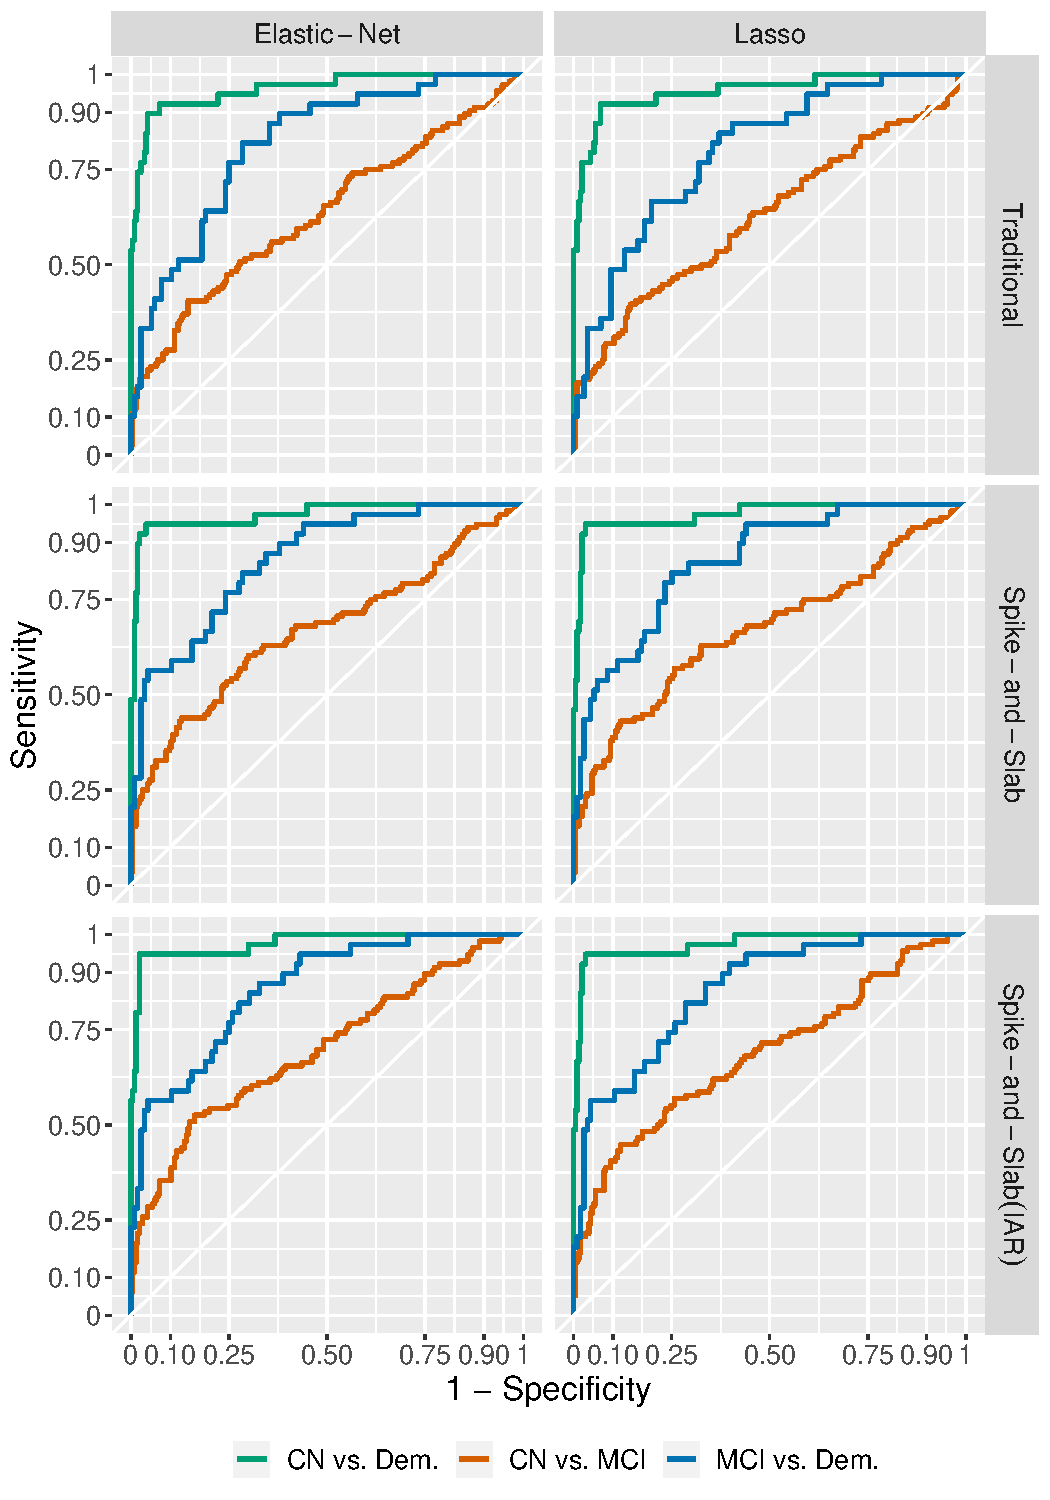
\includegraphics{analysis_details_files/figure-latex/unnamed-chunk-31-1.pdf}

This is Figure 4 from the paper (i.e., ROC curves for tau PET used as
features).

\begin{Shaded}
\begin{Highlighting}[]
\KeywordTok{ggplot}\NormalTok{(}\DataTypeTok{data =}\NormalTok{ all.tau.bl.yhat, }\KeywordTok{aes}\NormalTok{(}\DataTypeTok{d =}\NormalTok{ y.obs, }\DataTypeTok{m =}\NormalTok{ yhat.avg, }\DataTypeTok{color =}\NormalTok{ comparison)) }\OperatorTok{+}
\StringTok{  }\KeywordTok{geom_roc}\NormalTok{(}\DataTypeTok{labels =} \OtherTok{FALSE}\NormalTok{, }\DataTypeTok{n.cuts =} \DecValTok{0}\NormalTok{) }\OperatorTok{+}
\StringTok{  }\CommentTok{# geom_roc(labels = TRUE, cutoffs.at = c(0.25, 0.5, 0.75),}
\StringTok{  }\CommentTok{#          labelround = 2, labelsize = 3) +}
\StringTok{  }\KeywordTok{style_roc}\NormalTok{(}\DataTypeTok{theme =}\NormalTok{ theme_grey,}
            \DataTypeTok{ylab =} \StringTok{"Sensitivity"}\NormalTok{, }\DataTypeTok{xlab =} \StringTok{"1 - Specificity"}\NormalTok{) }\OperatorTok{+}
\StringTok{  }\KeywordTok{scale_y_continuous}\NormalTok{(}\DataTypeTok{name =} \StringTok{"Sensitivity"}\NormalTok{,}
                     \DataTypeTok{breaks =} \KeywordTok{c}\NormalTok{(}\DecValTok{0}\NormalTok{, }\FloatTok{0.1}\NormalTok{, }\FloatTok{0.25}\NormalTok{, }\FloatTok{0.5}\NormalTok{, }\FloatTok{0.75}\NormalTok{, }\FloatTok{0.9}\NormalTok{, }\DecValTok{1}\NormalTok{),}
                     \DataTypeTok{labels =} \KeywordTok{c}\NormalTok{(}\StringTok{"0"}\NormalTok{, }\StringTok{"0.10"}\NormalTok{, }\StringTok{"0.25"}\NormalTok{, }\StringTok{"0.50"}\NormalTok{, }\StringTok{"0.75"}\NormalTok{, }\StringTok{"0.90"}\NormalTok{, }\StringTok{"1"}\NormalTok{)) }\OperatorTok{+}
\StringTok{  }\KeywordTok{scale_x_continuous}\NormalTok{(}\DataTypeTok{name =} \StringTok{"1 - Specificity"}\NormalTok{,}
                     \DataTypeTok{breaks =} \KeywordTok{c}\NormalTok{(}\DecValTok{0}\NormalTok{, }\FloatTok{0.1}\NormalTok{, }\FloatTok{0.25}\NormalTok{, }\FloatTok{0.5}\NormalTok{, }\FloatTok{0.75}\NormalTok{, }\FloatTok{0.9}\NormalTok{, }\DecValTok{1}\NormalTok{),}
                     \DataTypeTok{labels =} \KeywordTok{c}\NormalTok{(}\StringTok{"0"}\NormalTok{, }\StringTok{"0.10"}\NormalTok{, }\StringTok{"0.25"}\NormalTok{, }\StringTok{"0.50"}\NormalTok{, }\StringTok{"0.75"}\NormalTok{, }\StringTok{"0.90"}\NormalTok{, }\StringTok{"1"}\NormalTok{)) }\OperatorTok{+}
\StringTok{  }\KeywordTok{facet_grid}\NormalTok{(model.lab}\OperatorTok{~}\NormalTok{alpha.lab2, }\DataTypeTok{labeller =} \KeywordTok{labeller}\NormalTok{(}\DataTypeTok{alpha.lab2 =}\NormalTok{ label_parsed,}
                                                       \DataTypeTok{model.lab =}\NormalTok{ label_parsed)) }\OperatorTok{+}
\StringTok{  }\KeywordTok{scale_color_manual}\NormalTok{(}\DataTypeTok{values =}\NormalTok{ cbp.b[}\KeywordTok{c}\NormalTok{(}\DecValTok{4}\NormalTok{, }\DecValTok{7}\NormalTok{, }\DecValTok{6}\NormalTok{)]) }\OperatorTok{+}
\StringTok{  }\KeywordTok{theme}\NormalTok{(}\DataTypeTok{plot.title =} \KeywordTok{element_text}\NormalTok{(}\DataTypeTok{hjust =} \FloatTok{0.5}\NormalTok{), }
        \DataTypeTok{text =} \KeywordTok{element_text}\NormalTok{(}\DataTypeTok{size =} \DecValTok{16}\NormalTok{),}
        \DataTypeTok{legend.position =} \StringTok{"bottom"}\NormalTok{,}
        \DataTypeTok{legend.title =} \KeywordTok{element_blank}\NormalTok{())  }
\end{Highlighting}
\end{Shaded}

\begin{verbatim}
## Scale for 'y' is already present. Adding another scale for 'y', which will
## replace the existing scale.
\end{verbatim}

\begin{verbatim}
## Scale for 'x' is already present. Adding another scale for 'x', which will
## replace the existing scale.
\end{verbatim}

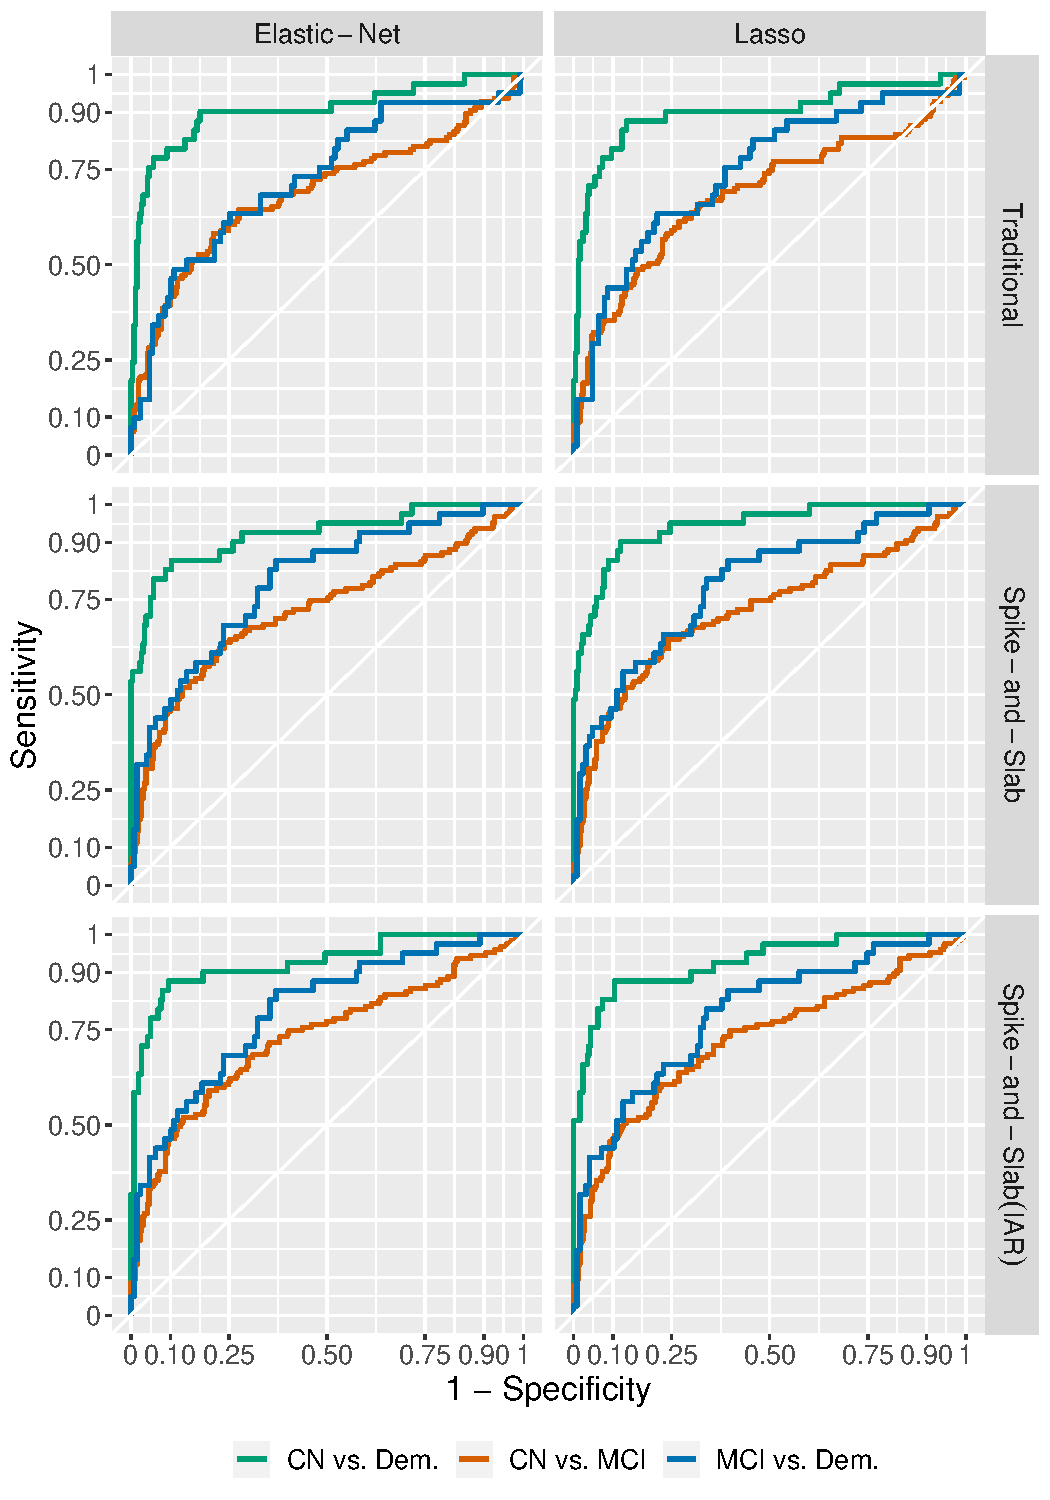
\includegraphics{analysis_details_files/figure-latex/unnamed-chunk-32-1.pdf}

\hypertarget{figures-for-classification-performance}{%
\subsection{Figures for Classification
Performance}\label{figures-for-classification-performance}}

We have a little bit of wrangling before plots.

\begin{Shaded}
\begin{Highlighting}[]
\NormalTok{resdir <-}\StringTok{ "C:/Users/Justin/Documents/BST/Dissertation_in_Latex/for-publishing/Rcode-ADNI/results_analyses_cheaha_scaled_2/"}
\CommentTok{# colorblind palettes}
\CommentTok{# colors: 1 grey/black 2 orange 3 light blue 4 green 5 yellow 6 dark blue 7 red-orange 8 pink }
\CommentTok{# The palette with grey:}
\NormalTok{cbp.g <-}\StringTok{ }\KeywordTok{c}\NormalTok{(}\StringTok{"#999999"}\NormalTok{, }\StringTok{"#E69F00"}\NormalTok{, }\StringTok{"#56B4E9"}\NormalTok{, }\StringTok{"#009E73"}\NormalTok{, }\StringTok{"#F0E442"}\NormalTok{, }\StringTok{"#0072B2"}\NormalTok{, }\StringTok{"#D55E00"}\NormalTok{, }\StringTok{"#CC79A7"}\NormalTok{)}

\CommentTok{# The palette with black:}
\NormalTok{cbp.b <-}\StringTok{ }\KeywordTok{c}\NormalTok{(}\StringTok{"#000000"}\NormalTok{, }\StringTok{"#E69F00"}\NormalTok{, }\StringTok{"#56B4E9"}\NormalTok{, }\StringTok{"#009E73"}\NormalTok{, }\StringTok{"#F0E442"}\NormalTok{, }\StringTok{"#0072B2"}\NormalTok{, }\StringTok{"#D55E00"}\NormalTok{, }\StringTok{"#CC79A7"}\NormalTok{)}

\CommentTok{# load results summaries}
\NormalTok{ct.smry <-}\StringTok{ }\KeywordTok{readRDS}\NormalTok{(}\DataTypeTok{file =} \KeywordTok{paste0}\NormalTok{(resdir, }\StringTok{"ct_smry.rds"}\NormalTok{))}
\NormalTok{ct.smry.ca <-}\StringTok{ }\NormalTok{ct.smry }\OperatorTok\StringTok{ }
\StringTok{  }\KeywordTok{select}\NormalTok{(outcome, model, alpha, s0, s1, accuracy, sensitivity, specificity, ppv, npv)}
\NormalTok{tau.smry <-}\StringTok{ }\KeywordTok{readRDS}\NormalTok{(}\DataTypeTok{file =} \KeywordTok{paste0}\NormalTok{(resdir, }\StringTok{"tau_smry.rds"}\NormalTok{))}
\NormalTok{tau.smry.ca <-}\StringTok{ }\NormalTok{tau.smry }\OperatorTok\StringTok{ }
\StringTok{  }\KeywordTok{select}\NormalTok{(outcome, model, alpha, s0, s1, accuracy, sensitivity, specificity, ppv, npv)}

\CommentTok{# Model names for figures}
\NormalTok{model <-}\StringTok{ }\KeywordTok{rep}\NormalTok{(}\KeywordTok{c}\NormalTok{(}\StringTok{"Lasso"}\NormalTok{, }\StringTok{"SSL"}\NormalTok{, }\StringTok{"SSL-IAR"}\NormalTok{,}
               \StringTok{"EN"}\NormalTok{, }\StringTok{"SSEN"}\NormalTok{, }\StringTok{"SSEN-IAR"}\NormalTok{),}
             \DecValTok{3}\NormalTok{)}

\CommentTok{# wrangle for figures}
\NormalTok{accuracy.wide <-}\StringTok{ }\KeywordTok{cbind}\NormalTok{(}\DataTypeTok{Model =}\NormalTok{ model,}
                       \DataTypeTok{Modality =} \KeywordTok{c}\NormalTok{(}\KeywordTok{rep}\NormalTok{(}\StringTok{"Cortical Thickness"}\NormalTok{, }\DecValTok{18}\NormalTok{), }\KeywordTok{rep}\NormalTok{(}\StringTok{"Tau PET"}\NormalTok{, }\DecValTok{18}\NormalTok{)) ,}
                       \KeywordTok{rbind}\NormalTok{(ct.smry.ca, tau.smry.ca)[, }\KeywordTok{c}\NormalTok{(}\DecValTok{1}\NormalTok{, }\DecValTok{6}\OperatorTok{:}\DecValTok{10}\NormalTok{)]}
\NormalTok{)}
\NormalTok{all.long <-}\StringTok{ }\KeywordTok{cbind}\NormalTok{(accuracy.wide[ , }\KeywordTok{c}\NormalTok{(}\DecValTok{1}\OperatorTok{:}\DecValTok{3}\NormalTok{)],}
                  \DataTypeTok{Estimate =} \KeywordTok{c}\NormalTok{(accuracy.wide}\OperatorTok{$}\NormalTok{accuracy, }
\NormalTok{                               accuracy.wide}\OperatorTok{$}\NormalTok{sensitivity,}
\NormalTok{                               accuracy.wide}\OperatorTok{$}\NormalTok{specificity,}
\NormalTok{                               accuracy.wide}\OperatorTok{$}\NormalTok{ppv,}
\NormalTok{                               accuracy.wide}\OperatorTok{$}\NormalTok{npv),}
                  \DataTypeTok{Assessment =} \KeywordTok{c}\NormalTok{(}\KeywordTok{rep}\NormalTok{(}\StringTok{"Accuracy"}\NormalTok{, }\DecValTok{36}\NormalTok{),}
                                 \KeywordTok{rep}\NormalTok{(}\StringTok{"Sensitivity"}\NormalTok{, }\DecValTok{36}\NormalTok{),}
                                 \KeywordTok{rep}\NormalTok{(}\StringTok{"Specificity"}\NormalTok{, }\DecValTok{36}\NormalTok{),}
                                 \KeywordTok{rep}\NormalTok{(}\StringTok{"PPV"}\NormalTok{, }\DecValTok{36}\NormalTok{),}
                                 \KeywordTok{rep}\NormalTok{(}\StringTok{"NPV"}\NormalTok{, }\DecValTok{36}\NormalTok{)))}
\KeywordTok{names}\NormalTok{(all.long) <-}\StringTok{ }\KeywordTok{c}\NormalTok{(}\StringTok{"Model"}\NormalTok{, }\StringTok{"Modality"}\NormalTok{, }\StringTok{"Comparison"}\NormalTok{, }\StringTok{"Estimate"}\NormalTok{, }\StringTok{"Assessment"}\NormalTok{)}
\NormalTok{all.long}\OperatorTok{$}\NormalTok{Model <-}\StringTok{ }\KeywordTok{factor}\NormalTok{(all.long}\OperatorTok{$}\NormalTok{Model, }
                         \DataTypeTok{levels =} \KeywordTok{c}\NormalTok{(}\StringTok{"Lasso"}\NormalTok{, }\StringTok{"SSL"}\NormalTok{, }\StringTok{"SSL-IAR"}\NormalTok{,}
                                    \StringTok{"EN"}\NormalTok{, }\StringTok{"SSEN"}\NormalTok{, }\StringTok{"SSEN-IAR"}\NormalTok{))}
\NormalTok{all.long}\OperatorTok{$}\NormalTok{Assessment <-}\StringTok{ }\KeywordTok{factor}\NormalTok{(all.long}\OperatorTok{$}\NormalTok{Assessment,}
                              \DataTypeTok{levels =} \KeywordTok{c}\NormalTok{(}\StringTok{"Accuracy"}\NormalTok{, }\StringTok{"Sensitivity"}\NormalTok{, }\StringTok{"Specificity"}\NormalTok{, }\StringTok{"PPV"}\NormalTok{, }\StringTok{"NPV"}\NormalTok{))}

\CommentTok{# I think this `set.seed()` argument was here by accident.}
\CommentTok{# I can't find a use for it, but left it commented out just in case.}
\CommentTok{# set.seed(5845549)}
\end{Highlighting}
\end{Shaded}

This is Figure 5 from the paper (i.e., performance for classifying
cognitive normal vs.~dementia subjects).

\begin{Shaded}
\begin{Highlighting}[]
\CommentTok{# CN vs. D}
\NormalTok{cnd.long <-}\StringTok{ }\NormalTok{all.long }\OperatorTok\StringTok{ }
\StringTok{  }\KeywordTok{filter}\NormalTok{(Comparison }\OperatorTok{==}\StringTok{ "CN vs. Dem."}\NormalTok{)}

\KeywordTok{ggplot}\NormalTok{(}\DataTypeTok{data =}\NormalTok{ cnd.long,}
       \DataTypeTok{mapping =} \KeywordTok{aes}\NormalTok{(}\DataTypeTok{y =}\NormalTok{ Estimate,}
                     \DataTypeTok{x =}\NormalTok{ Model, }
                     \DataTypeTok{colour =}\NormalTok{ Assessment,}
                     \DataTypeTok{shape =}\NormalTok{ Assessment)) }\OperatorTok{+}
\StringTok{  }\KeywordTok{geom_point}\NormalTok{(}\DataTypeTok{size =} \DecValTok{3}\NormalTok{, }\DataTypeTok{stroke =} \FloatTok{1.5}\NormalTok{) }\OperatorTok{+}
\StringTok{  }\KeywordTok{scale_shape_manual}\NormalTok{(}\DataTypeTok{values =} \KeywordTok{c}\NormalTok{(}\DecValTok{8}\NormalTok{, }\DecValTok{15}\NormalTok{, }\DecValTok{17}\NormalTok{, }\DecValTok{18}\NormalTok{, }\DecValTok{25}\NormalTok{)) }\OperatorTok{+}
\StringTok{  }\KeywordTok{scale_color_manual}\NormalTok{(}\DataTypeTok{values =}\NormalTok{ cbp.b[}\KeywordTok{c}\NormalTok{(}\DecValTok{1}\NormalTok{, }\DecValTok{2}\NormalTok{, }\DecValTok{4}\NormalTok{, }\DecValTok{7}\NormalTok{, }\DecValTok{6}\NormalTok{)]) }\OperatorTok{+}
\StringTok{  }\CommentTok{# scale_fill_manual(values = cbp.b[c(1, 2, 4, 7, 3 )]) +}
\StringTok{  }\KeywordTok{facet_wrap}\NormalTok{(cnd.long}\OperatorTok{$}\NormalTok{Modality) }\OperatorTok{+}
\StringTok{  }\KeywordTok{scale_x_discrete}\NormalTok{(}\DataTypeTok{name =} \OtherTok{NULL}\NormalTok{) }\OperatorTok{+}
\StringTok{  }\KeywordTok{scale_y_continuous}\NormalTok{(}\DataTypeTok{limits =} \KeywordTok{c}\NormalTok{(}\FloatTok{0.4}\NormalTok{, }\DecValTok{1}\NormalTok{),}
                     \DataTypeTok{breaks =} \KeywordTok{seq}\NormalTok{(}\FloatTok{0.4}\NormalTok{, }\DecValTok{1}\NormalTok{, }\FloatTok{0.1}\NormalTok{)) }\OperatorTok{+}
\StringTok{  }\KeywordTok{theme}\NormalTok{(}\DataTypeTok{plot.title =} \KeywordTok{element_text}\NormalTok{(}\DataTypeTok{hjust =} \FloatTok{0.5}\NormalTok{), }
        \DataTypeTok{text =} \KeywordTok{element_text}\NormalTok{(}\DataTypeTok{size =} \DecValTok{14}\NormalTok{),}
        \DataTypeTok{legend.position =} \StringTok{"bottom"}\NormalTok{)}
\end{Highlighting}
\end{Shaded}

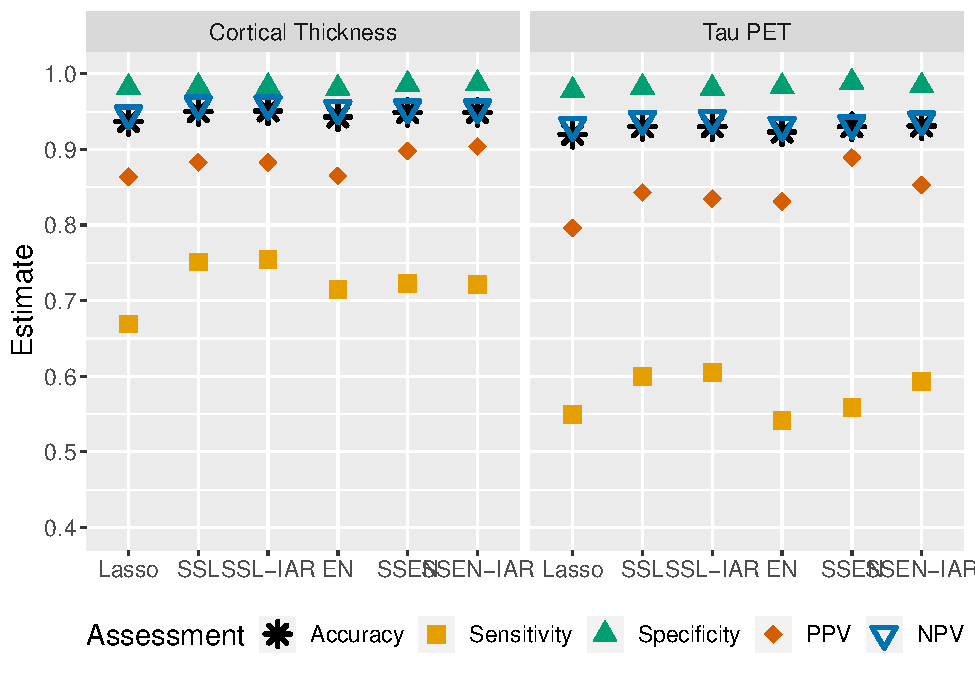
\includegraphics{analysis_details_files/figure-latex/unnamed-chunk-34-1.pdf}

This is Figure 6 from the paper (i.e., performance for classifying
cognitive normal vs.~MCI subjects).

\begin{Shaded}
\begin{Highlighting}[]
\CommentTok{# CN vs. MCI}
\NormalTok{cnmci.long <-}\StringTok{ }\NormalTok{all.long }\OperatorTok
\StringTok{  }\KeywordTok{filter}\NormalTok{(Comparison }\OperatorTok{==}\StringTok{ "CN vs. MCI"}\NormalTok{)}
\KeywordTok{ggplot}\NormalTok{(}\DataTypeTok{data =}\NormalTok{ cnmci.long,}
       \DataTypeTok{mapping =} \KeywordTok{aes}\NormalTok{(}\DataTypeTok{y =}\NormalTok{ Estimate,}
                     \DataTypeTok{x =}\NormalTok{ Model, }
                     \DataTypeTok{colour =}\NormalTok{ Assessment,}
                     \DataTypeTok{shape =}\NormalTok{ Assessment)) }\OperatorTok{+}
\StringTok{  }\KeywordTok{geom_point}\NormalTok{(}\DataTypeTok{size =} \DecValTok{3}\NormalTok{, }\DataTypeTok{stroke =} \FloatTok{1.5}\NormalTok{) }\OperatorTok{+}
\StringTok{  }\KeywordTok{scale_shape_manual}\NormalTok{(}\DataTypeTok{values =} \KeywordTok{c}\NormalTok{(}\DecValTok{8}\NormalTok{, }\DecValTok{15}\NormalTok{, }\DecValTok{17}\NormalTok{, }\DecValTok{18}\NormalTok{, }\DecValTok{25}\NormalTok{)) }\OperatorTok{+}
\StringTok{  }\KeywordTok{scale_color_manual}\NormalTok{(}\DataTypeTok{values =}\NormalTok{ cbp.b[}\KeywordTok{c}\NormalTok{(}\DecValTok{1}\NormalTok{, }\DecValTok{2}\NormalTok{, }\DecValTok{4}\NormalTok{, }\DecValTok{7}\NormalTok{, }\DecValTok{6}\NormalTok{)]) }\OperatorTok{+}
\StringTok{  }\CommentTok{# scale_fill_manual(values = cbp.b[c(1, 2, 4, 7, 3 )]) +}
\StringTok{  }\KeywordTok{facet_wrap}\NormalTok{(cnd.long}\OperatorTok{$}\NormalTok{Modality) }\OperatorTok{+}
\StringTok{  }\KeywordTok{scale_x_discrete}\NormalTok{(}\DataTypeTok{name =} \OtherTok{NULL}\NormalTok{) }\OperatorTok{+}
\StringTok{  }\KeywordTok{scale_y_continuous}\NormalTok{(}\DataTypeTok{limits =} \KeywordTok{c}\NormalTok{(}\FloatTok{0.18}\NormalTok{, }\DecValTok{1}\NormalTok{),}
                     \DataTypeTok{breaks =} \KeywordTok{seq}\NormalTok{(}\FloatTok{0.2}\NormalTok{, }\DecValTok{1}\NormalTok{, }\FloatTok{0.1}\NormalTok{)) }\OperatorTok{+}
\StringTok{  }\KeywordTok{theme}\NormalTok{(}\DataTypeTok{plot.title =} \KeywordTok{element_text}\NormalTok{(}\DataTypeTok{hjust =} \FloatTok{0.5}\NormalTok{), }
        \DataTypeTok{text =} \KeywordTok{element_text}\NormalTok{(}\DataTypeTok{size =} \DecValTok{14}\NormalTok{),}
        \DataTypeTok{legend.position =} \StringTok{"bottom"}\NormalTok{)}
\end{Highlighting}
\end{Shaded}

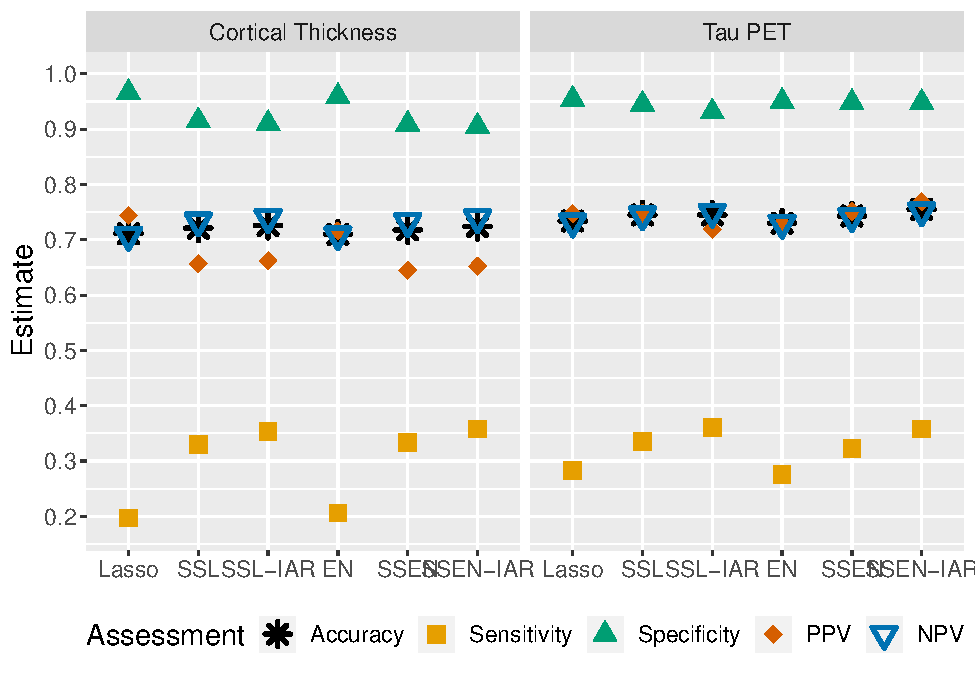
\includegraphics{analysis_details_files/figure-latex/unnamed-chunk-35-1.pdf}

This is Figure 7 from the paper (i.e., performance for classifying MCI
vs.~dementia subjects).

\begin{Shaded}
\begin{Highlighting}[]
\CommentTok{# MCI vs. D}
\NormalTok{mcid.long <-}\StringTok{ }\NormalTok{all.long }\OperatorTok\StringTok{ }
\StringTok{  }\KeywordTok{filter}\NormalTok{(Comparison }\OperatorTok{==}\StringTok{ "MCI vs. Dem."}\NormalTok{)}
\KeywordTok{ggplot}\NormalTok{(}\DataTypeTok{data =}\NormalTok{ mcid.long,}
       \DataTypeTok{mapping =} \KeywordTok{aes}\NormalTok{(}\DataTypeTok{y =}\NormalTok{ Estimate,}
                     \DataTypeTok{x =}\NormalTok{ Model, }
                     \DataTypeTok{colour =}\NormalTok{ Assessment,}
                     \DataTypeTok{shape =}\NormalTok{ Assessment)) }\OperatorTok{+}
\StringTok{  }\KeywordTok{geom_point}\NormalTok{(}\DataTypeTok{size =} \DecValTok{3}\NormalTok{, }\DataTypeTok{stroke =} \FloatTok{1.5}\NormalTok{) }\OperatorTok{+}
\StringTok{  }\KeywordTok{scale_shape_manual}\NormalTok{(}\DataTypeTok{values =} \KeywordTok{c}\NormalTok{(}\DecValTok{8}\NormalTok{, }\DecValTok{15}\NormalTok{, }\DecValTok{17}\NormalTok{, }\DecValTok{18}\NormalTok{, }\DecValTok{25}\NormalTok{)) }\OperatorTok{+}
\StringTok{  }\KeywordTok{scale_color_manual}\NormalTok{(}\DataTypeTok{values =}\NormalTok{ cbp.b[}\KeywordTok{c}\NormalTok{(}\DecValTok{1}\NormalTok{, }\DecValTok{2}\NormalTok{, }\DecValTok{4}\NormalTok{, }\DecValTok{7}\NormalTok{, }\DecValTok{6}\NormalTok{)]) }\OperatorTok{+}
\StringTok{  }\CommentTok{# scale_fill_manual(values = cbp.b[c(1, 2, 4, 7, 3 )]) +}
\StringTok{  }\KeywordTok{facet_wrap}\NormalTok{(cnd.long}\OperatorTok{$}\NormalTok{Modality) }\OperatorTok{+}
\StringTok{  }\KeywordTok{scale_x_discrete}\NormalTok{(}\DataTypeTok{name =} \OtherTok{NULL}\NormalTok{) }\OperatorTok{+}
\StringTok{  }\KeywordTok{scale_y_continuous}\NormalTok{(}\DataTypeTok{limits =} \KeywordTok{c}\NormalTok{(}\FloatTok{0.15}\NormalTok{, }\DecValTok{1}\NormalTok{),}
                     \DataTypeTok{breaks =} \KeywordTok{seq}\NormalTok{(}\FloatTok{0.2}\NormalTok{, }\DecValTok{1}\NormalTok{, }\FloatTok{0.1}\NormalTok{)) }\OperatorTok{+}
\StringTok{  }\KeywordTok{theme}\NormalTok{(}\DataTypeTok{plot.title =} \KeywordTok{element_text}\NormalTok{(}\DataTypeTok{hjust =} \FloatTok{0.5}\NormalTok{), }
        \DataTypeTok{text =} \KeywordTok{element_text}\NormalTok{(}\DataTypeTok{size =} \DecValTok{14}\NormalTok{),}
        \DataTypeTok{legend.position =} \StringTok{"bottom"}\NormalTok{)}
\end{Highlighting}
\end{Shaded}

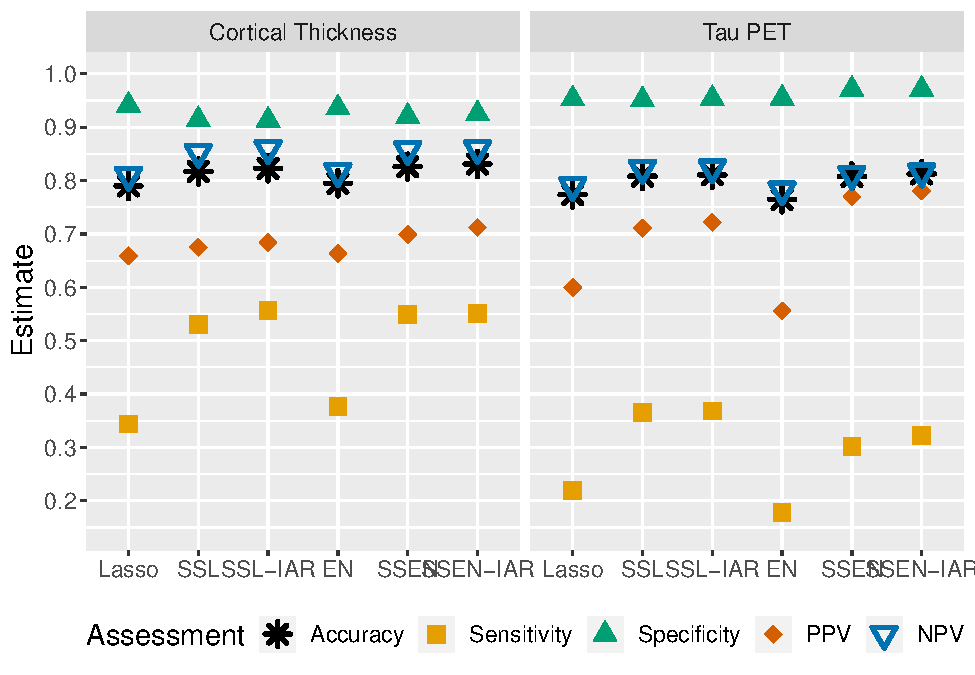
\includegraphics{analysis_details_files/figure-latex/unnamed-chunk-36-1.pdf}

\end{document}
